\hypertarget{ch3}{\chapter{Application of selected statistical models on COVID-19 related time series}}

This chapter aims at the practical application of the statistical models introduced in Chapter \hyperlink{ch2}{2} in the context of modeling time series related to the COVID-19 pandemic in the Czech Republic.

\section{Data}

One of the most determining steps in data analysis is the searching, selection, and preparation of reliable data.

\subsection{Data sources}

The main practical goal of this thesis is to perform an analysis of time series generated by different processes related to the COVID-19 pandemic in the Czech Republic. According to this fact, the fundamental data source for this work is the official website created in association with the Ministry of Health of the Czech Republic with information about it \cite{covidczdata}.

\subsection{Data selection}

After inspection of the available data and exploring different articles that aim at the modeling of COVID-19 pandemic time series in various countries all around the world, we decided to select the time series that describe \textbf{the cumulative number of people infected}, \textbf{the cumulative number of people cured}, \textbf{the cumulative number of people dead}, and \textbf{the number of active cases}.

All selected data frames were last updated on May 4, 2021 and store measurements obtained from March 1, 2020. 

\subsection{Data preparation}

All data were obtained from an official and reliable web source. Thus, there were no consistency data problems such as missing or invalid values. However, there was no time series with information about the active cases ($A$), so it was aggregated from time series that describe the number of people infected ($I$), cured ($C$), and dead ($D$) using the following formula
\begin{equation}
    A = I - C - D.
\end{equation}
After doing that, it is necessary to transform each data frame into a form compatible with the Facebook Prophet model. Table \ref{tab:cum_inf_example_table} demonstrates the time series with information about the number of people infected daily in its final form.

\begin{table}[!ht]
    \centering
    \begin{tabular}{|p{3cm}|p{3cm}|}
    \hline
     \multicolumn{2}{|c|}{\textbf{Cumulative number of people infected
     }} \\
    \hline
    \textbf{ds} & \textbf{y}\\
    \hline
    2020-03-01 & 3\\
    \hline
	2020-03-02 & 3\\
	\hline
	2020-03-03 & 5\\
	\hline
	2020-03-04 & 6\\
	\hline
    2020-03-05 & 9\\
 \hline
\end{tabular}
    \caption{Final form of the data frame with information about cumulative amount of people infected.}
    \label{tab:cum_inf_example_table}
\end{table}

\hypertarget{s3.2}{\section{Basic analysis of the selected time series}}

After preparing all the selected time series, we need to perform their basic analysis to 
\begin{itemize}
    \item find some interesting phenomena, possible seasonal or cyclic patterns,
    \item estimate the order of future SARIMA models,
    \item perform basic statistical testing (stationarity tests).
\end{itemize}
Now, we can perform an analysis of each time series individually.

\begin{figure}[!ht]
\centering
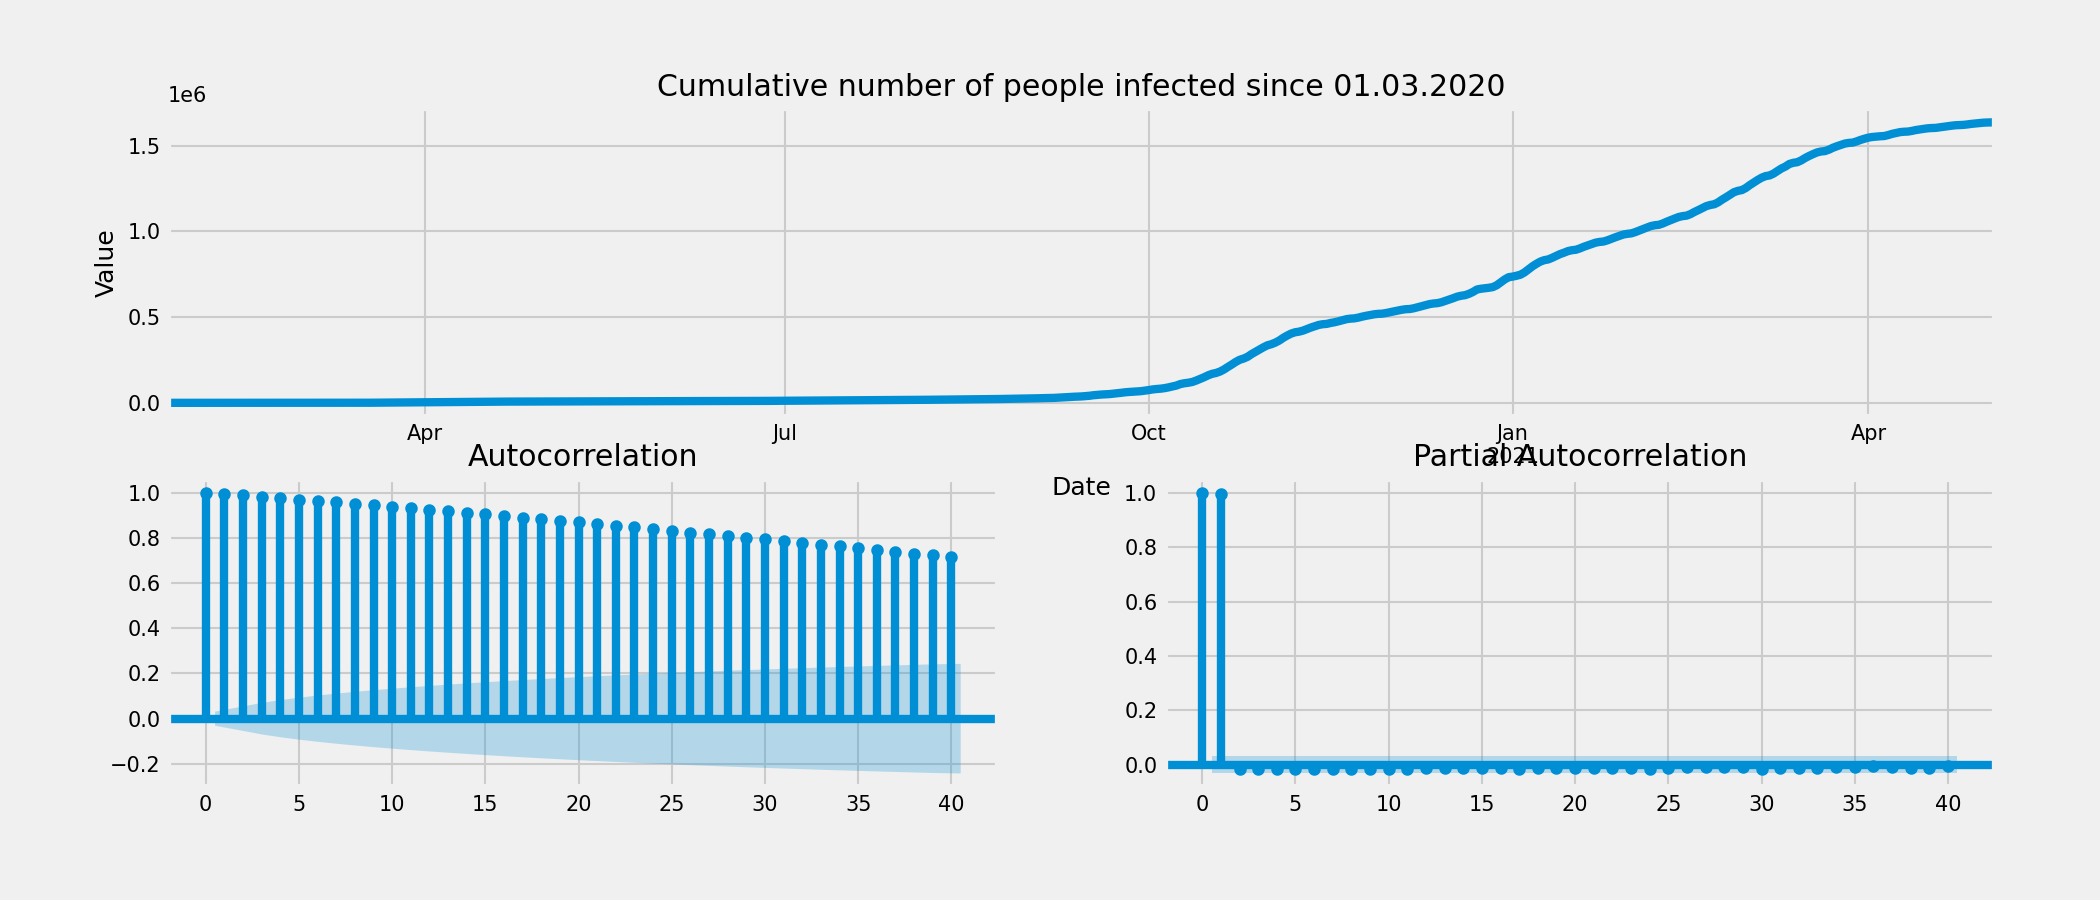
\includegraphics[width=1\textwidth, height=0.35\textwidth]{figures/chapter_04/original_ts/ts_orig_infected.png}
\caption{The cumulative number of people infected in Czech Republic time series with the corresponding ACF and PACF.}
\label{fig:orin_infected}
\end{figure}
\begin{figure}[!htb]
  \centering
  \subfloat[a][The cumulative number of people infected time series after differencing at lag 1.]{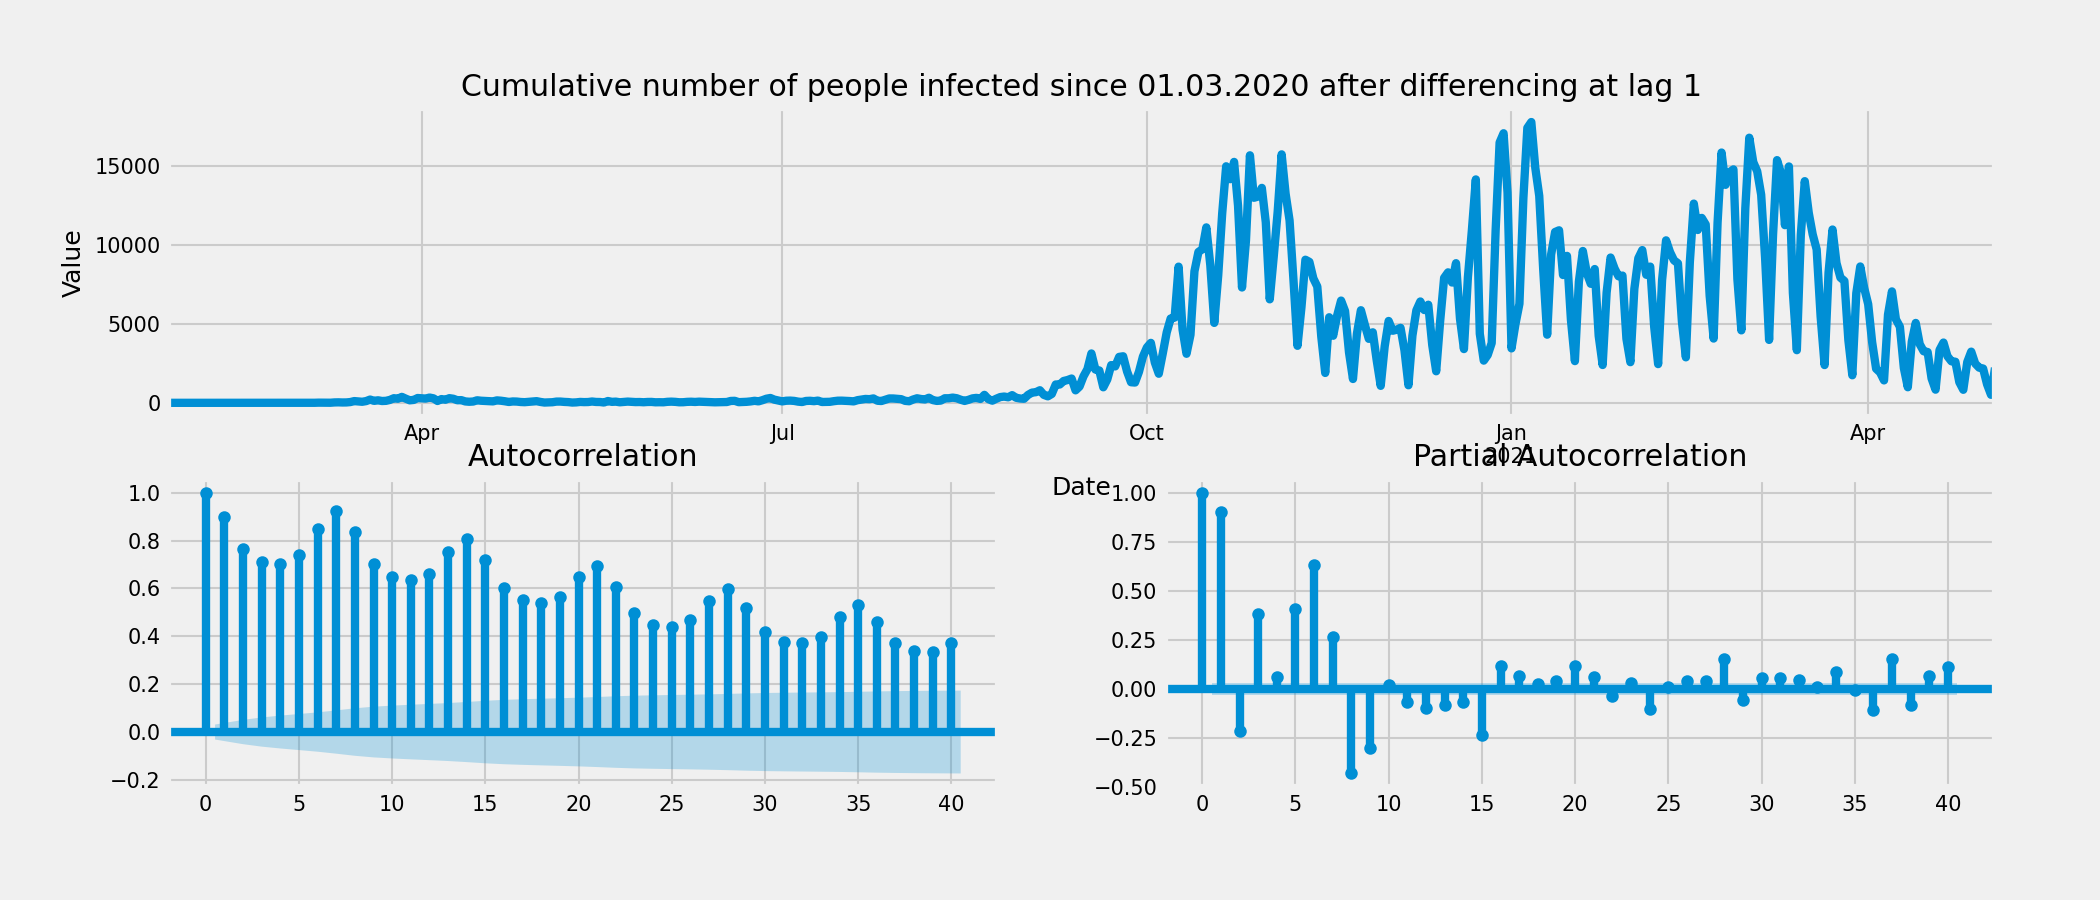
\includegraphics[width=1\textwidth, height=0.3\textwidth]{figures/chapter_04/infected_ts/ts_diff_infected.png}
  \label{fig:infected_diff}} \\
  \subfloat[b][The cumulative number of people infected time series after double differencing at lag 1.]{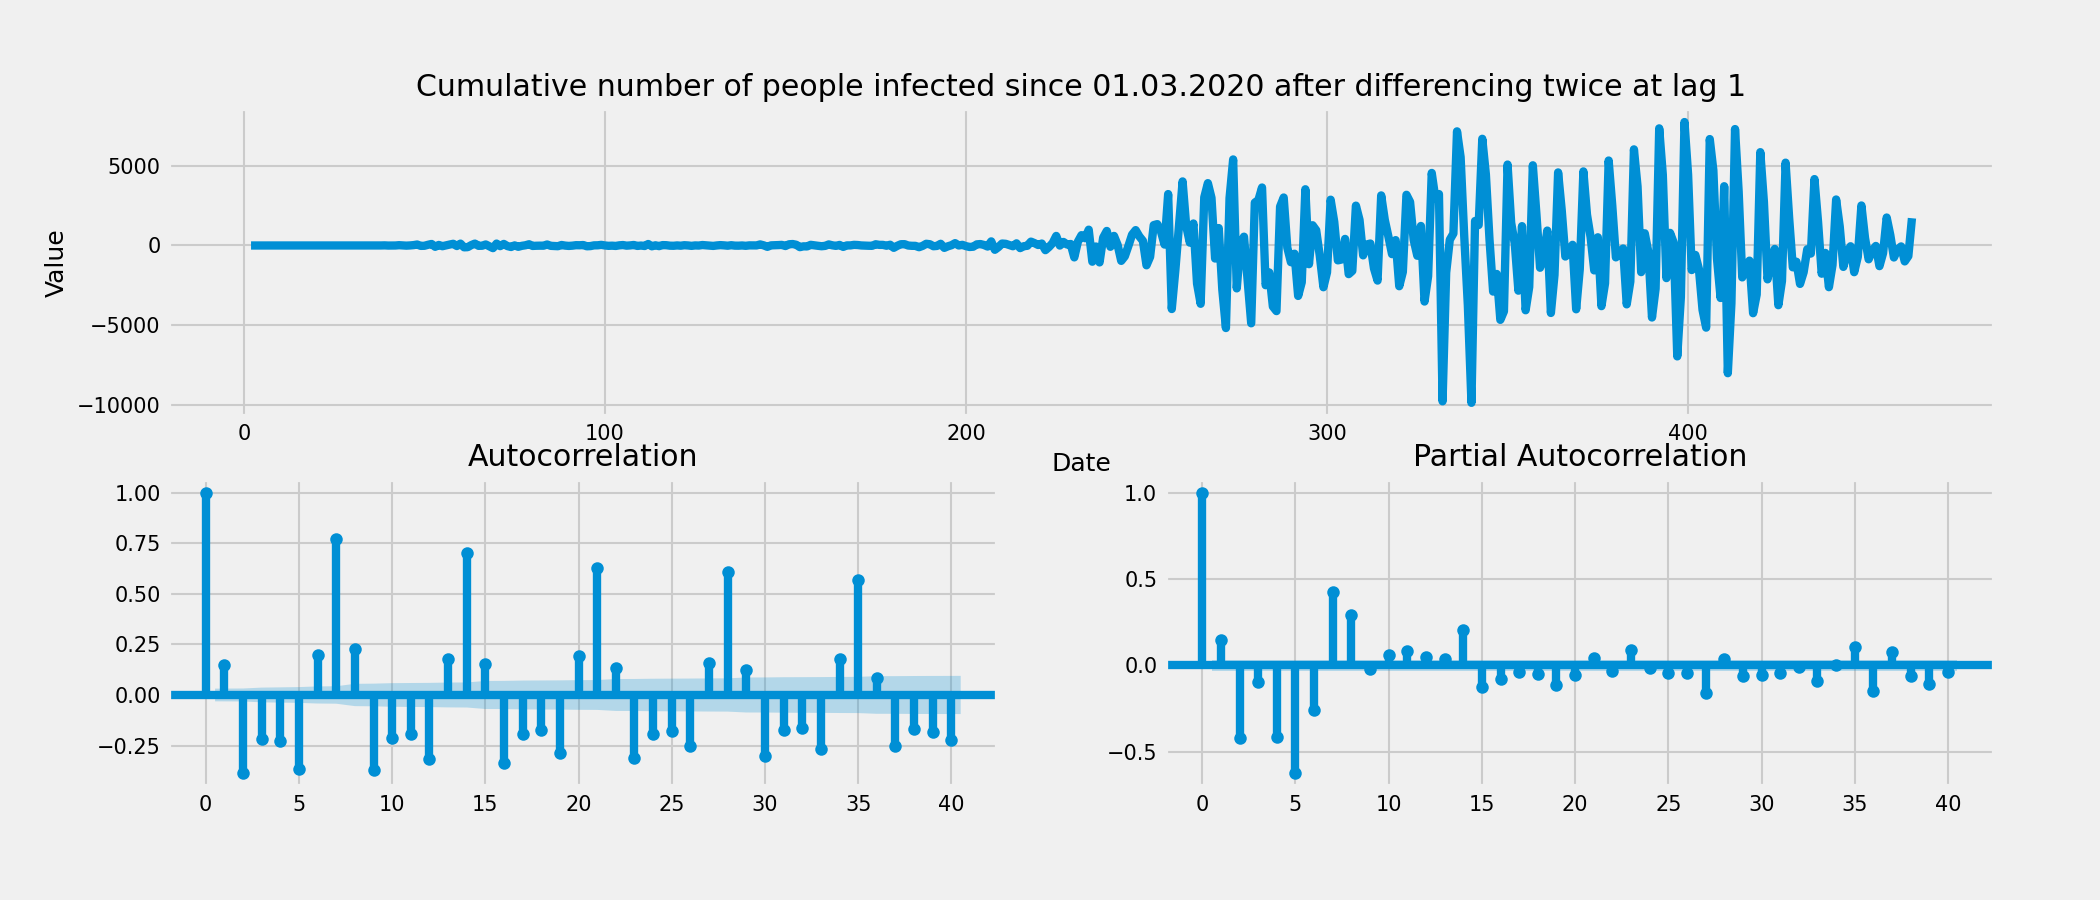
\includegraphics[width=1\textwidth, height=0.3\textwidth]{figures/chapter_04/infected_ts/ts_diff1_1_infected.png}
  \label{fig:infected_diff_1_1}} \\
  \subfloat[c][The cumulative number of people infected time series after differencing at lag 1 and 7.]{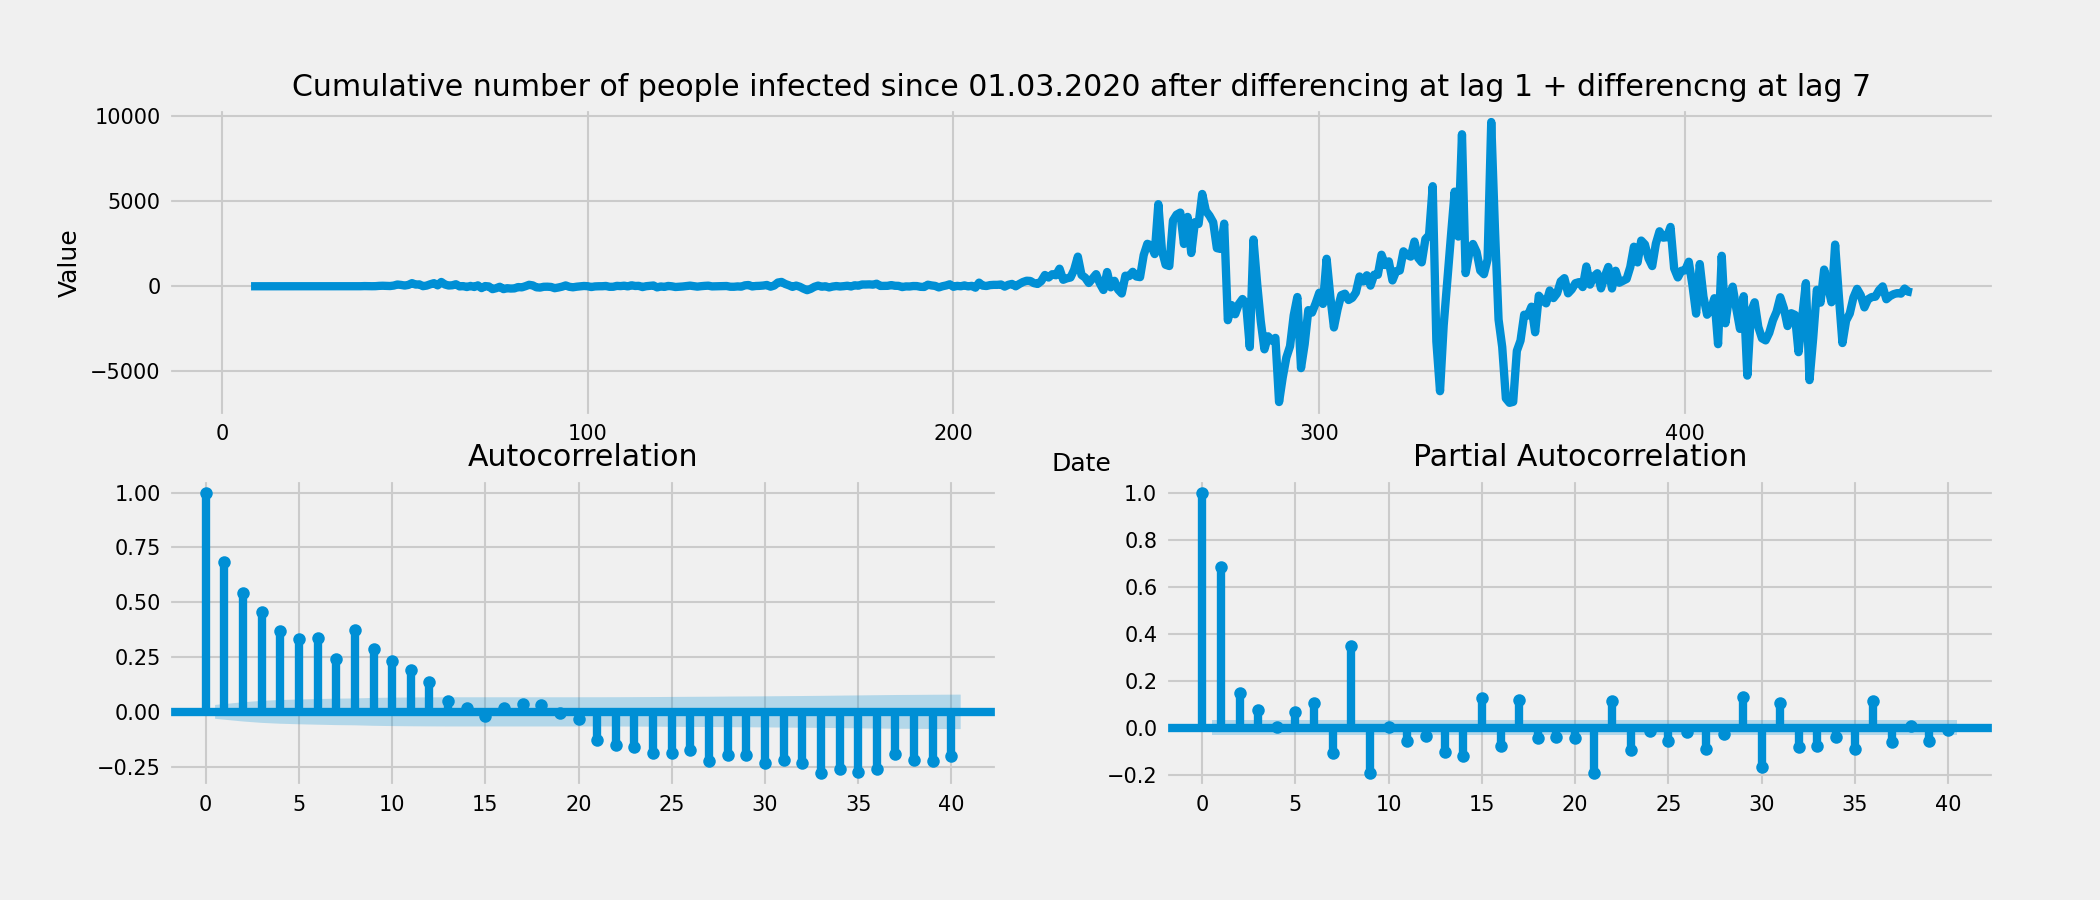
\includegraphics[width=1\textwidth, height=0.3\textwidth]{figures/chapter_04/infected_ts/ts_diff1_7_infected.png}
  \label{fig:infected_diff_1_7}}
  \caption{The cumulative amount of people infected after different differencing sequences with the corresponding ACF and PACF.}
  \label{fig:infected_diff_ex}
\end{figure}

\subsection{Cumulative number of people infected daily time series}

First, we will inspect the cumulative number of people infected time series.

Figure \ref{fig:orin_infected} demonstrates the original time series that describes the cumulative number of people infected daily with the corresponding ACF and PACF. It is clear that this time series is a cumulative sum, so it does not give any valuable information. Thus, we need to perform differencing at lag 1.

Now we can see (Figure \ref{fig:infected_diff}) the following interesting properties of this time series:
\begin{itemize}
    \item There is no interesting activity until the beginning of June. It means that we can drop the first part of the time series during the modeling process.
    \item According to the ACF, there is a global trend (the correlation measure slowly decreases) and weekly seasonality (peaks at lags 7, 14, 21, and so on).
    \item According to the stationarity tests (Table 3.2), this is a nonstationary time series.
\end{itemize}
This leads to the fact that we need to get rid of nonstationarity. However, it is possible in two ways: one more differencing at lag 1 or seasonal differencing at lag 7. 

In Figure \ref{fig:infected_diff_1_1} and Figure \ref{fig:infected_diff_1_7} you can see the time series after double differencing at lag 1 and after one-time differencing at lag 1 and lag 7, respectively. 

In the first case, we got rid of the global trend, but we still have seasonality (significant correlation at lag 7, 14, and so on). Moreover, Table \ref{tab:infected_tests_table} indicates that the time series is now stationary. The ACF shows that the possible seasonal autoregressive order is 1.

In the second case, we got rid of the seasonality. Stationarity tests (Table \ref{tab:infected_tests_table}) indicate that the time series is now stationary. The ACF and PACF show that the possible autoregressive order is 1.

All this information follows that the cumulative number of people infected time series is generated by the process that can be described by SARIMA(1, 2, 0) $\times$ (1, 0, 0$)_7$ or SARIMA(1, 1, 0) $\times$ (1, 1, 0$)_7$ models.

\begin{table}[!ht]
    \centering
    \begin{tabular}{|p{3cm}||p{3cm}| p{3cm}|}
    \hline
    Time series & Dikey-Fuller test p-value & KPSS test p-value\\
    \hline
    Original time series& 0.993501 & 0.010000\\
    \hline
    1x at lag 1 & 0.295332 & 0.010000\\
	\hline
	2x at lag 1 & 0.001123 & 0.100000\\
	\hline
	1x lag 1; 1x at lag 7 & 0.001654 & 0.100000\\
 \hline
\end{tabular}
    \caption{The Cumulative number of people infected: results of the stationarity tests.}
    \label{tab:infected_tests_table}
\end{table}

\subsection{The cumulative number of people cured time series}

Figure \ref{fig:orig_cured} demonstrates the original time series that describes the cumulative number of people cured daily with the corresponding ACF and PACF. Similar to the previous time series, it is a cumulative sum. Thus, we need to perform differencing at lag 1. 

Figure \ref{fig:cured_diff} shows the time series after the first differencing. We can see the global trend and weekly seasonality. The ACF and PACF also demonstrate a slowly decreasing measure of correlation. Additionally, the ACF shows peaks at lags 7, 14, 21, and so on (seasonality). In Table \ref{tab:cured_tests_table} we can find out that this time series is nonstationary, and we need to do one more differencing. 

\begin{table}[!ht]
    \centering
    \begin{tabular}{|p{3cm}||p{3cm}| p{3cm}|}
    \hline
    Time series & Dikey-Fuller test p-value & KPSS test p-value\\
    \hline
    Original time series& 0.928839 & 0.010000\\
	\hline
	1x at lag 1 & 0.120930 & 0.010000\\
	\hline
	2x at lag 1 &  0.000021 & 0.100000\\
	\hline
	1x lag 1; 1x at lag 7 & 0.000027 & 0.100000\\
 \hline
\end{tabular}
    \caption{The Cumulative number of people cured: results of the stationarity tests.}
    \label{tab:cured_tests_table}
\end{table}

\begin{figure}[!htb]
  \centering
  \subfloat[a][The original cumulative number of people cured time series.]{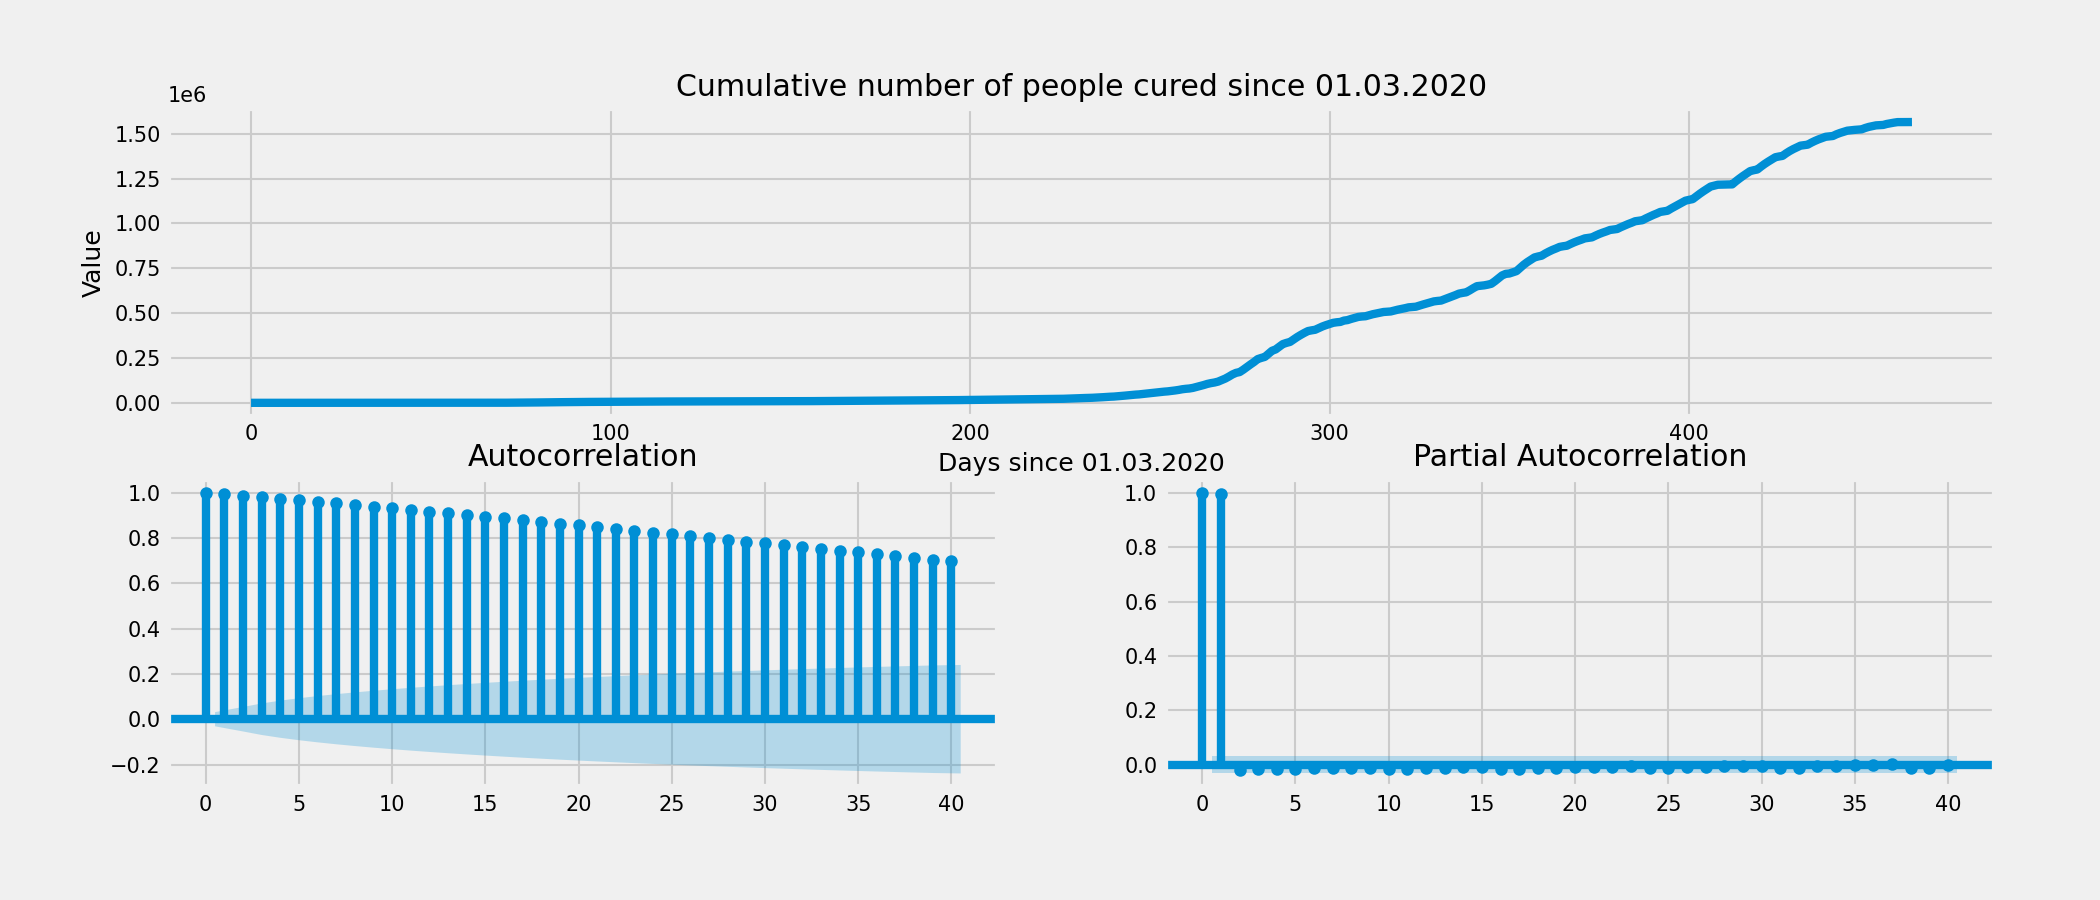
\includegraphics[width=1\textwidth, height=0.28\textwidth]{figures/chapter_04/original_ts/ts_orig_cured.png}
  \label{fig:orig_cured}} \\
  \subfloat[b][The cumulative number of people cured time series after differencing at lag 1.]{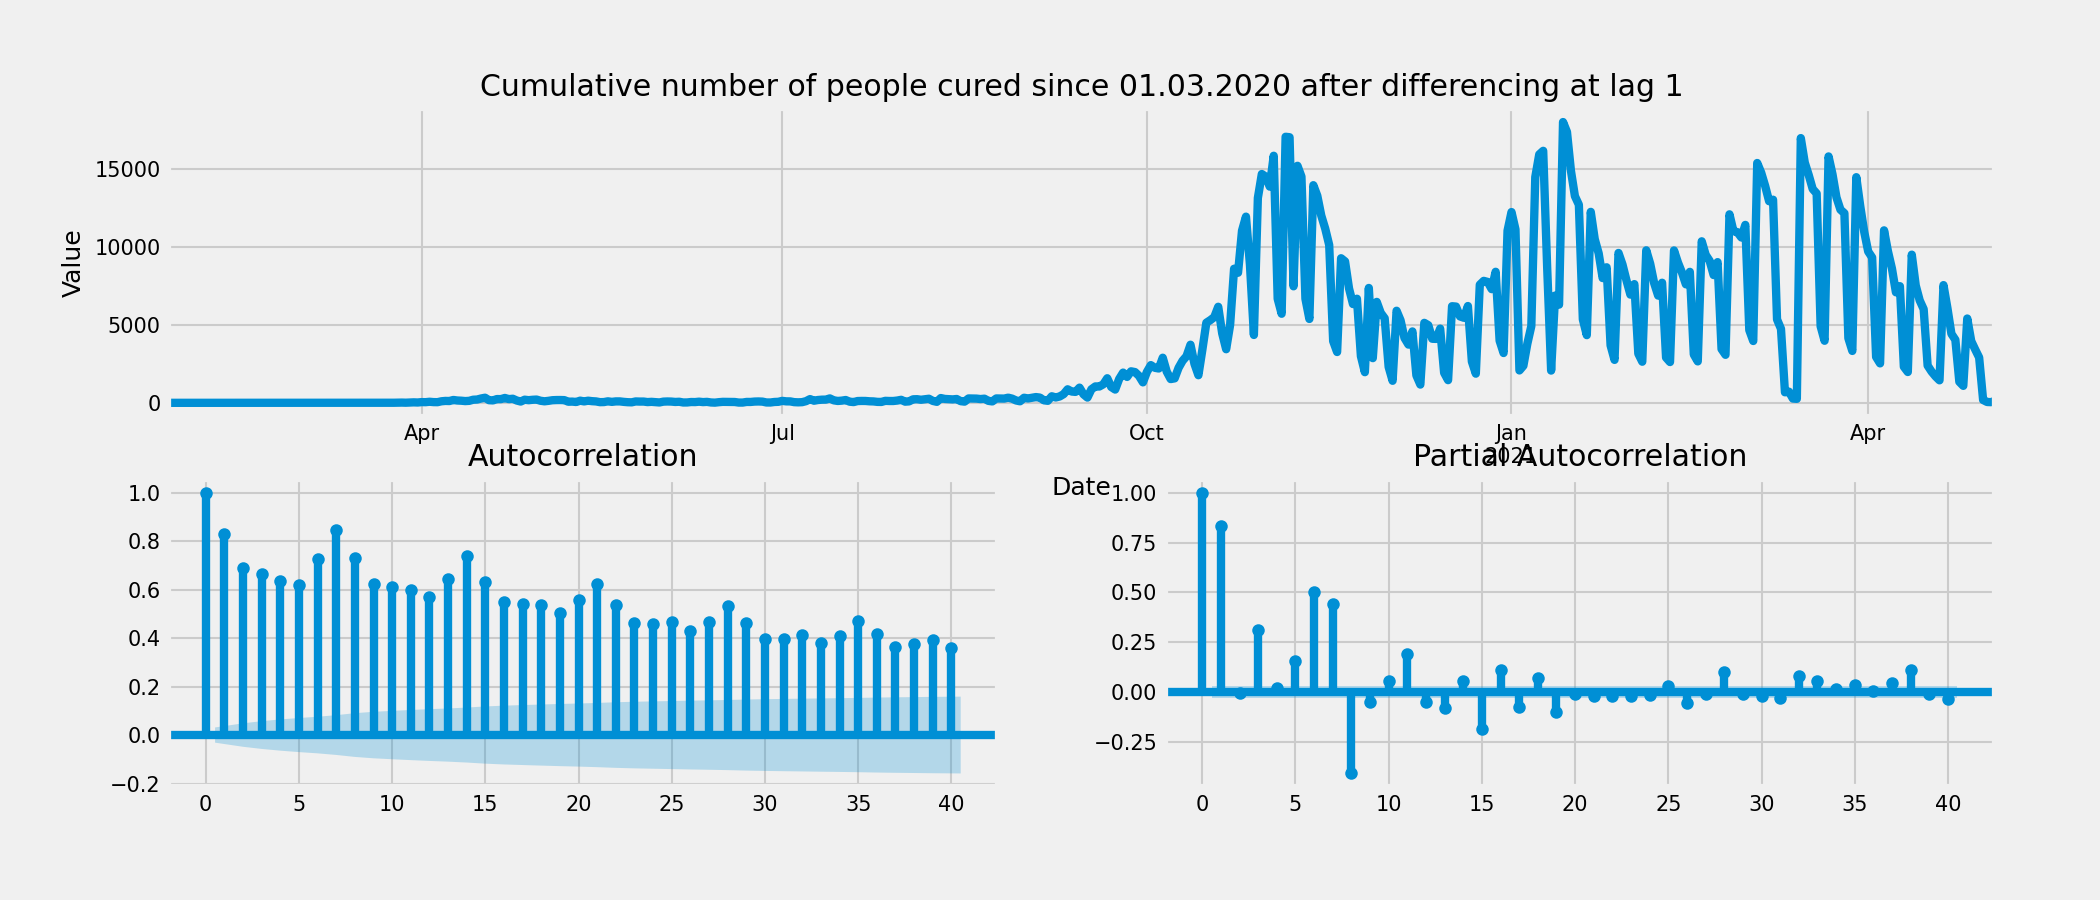
\includegraphics[width=1\textwidth, height=0.28\textwidth]{figures/chapter_04/cured_ts/ts_diff_cured.png}
  \label{fig:cured_diff}} \\
  \subfloat[c][The cumulative number of people cured time series after double differencing at lag 1.]{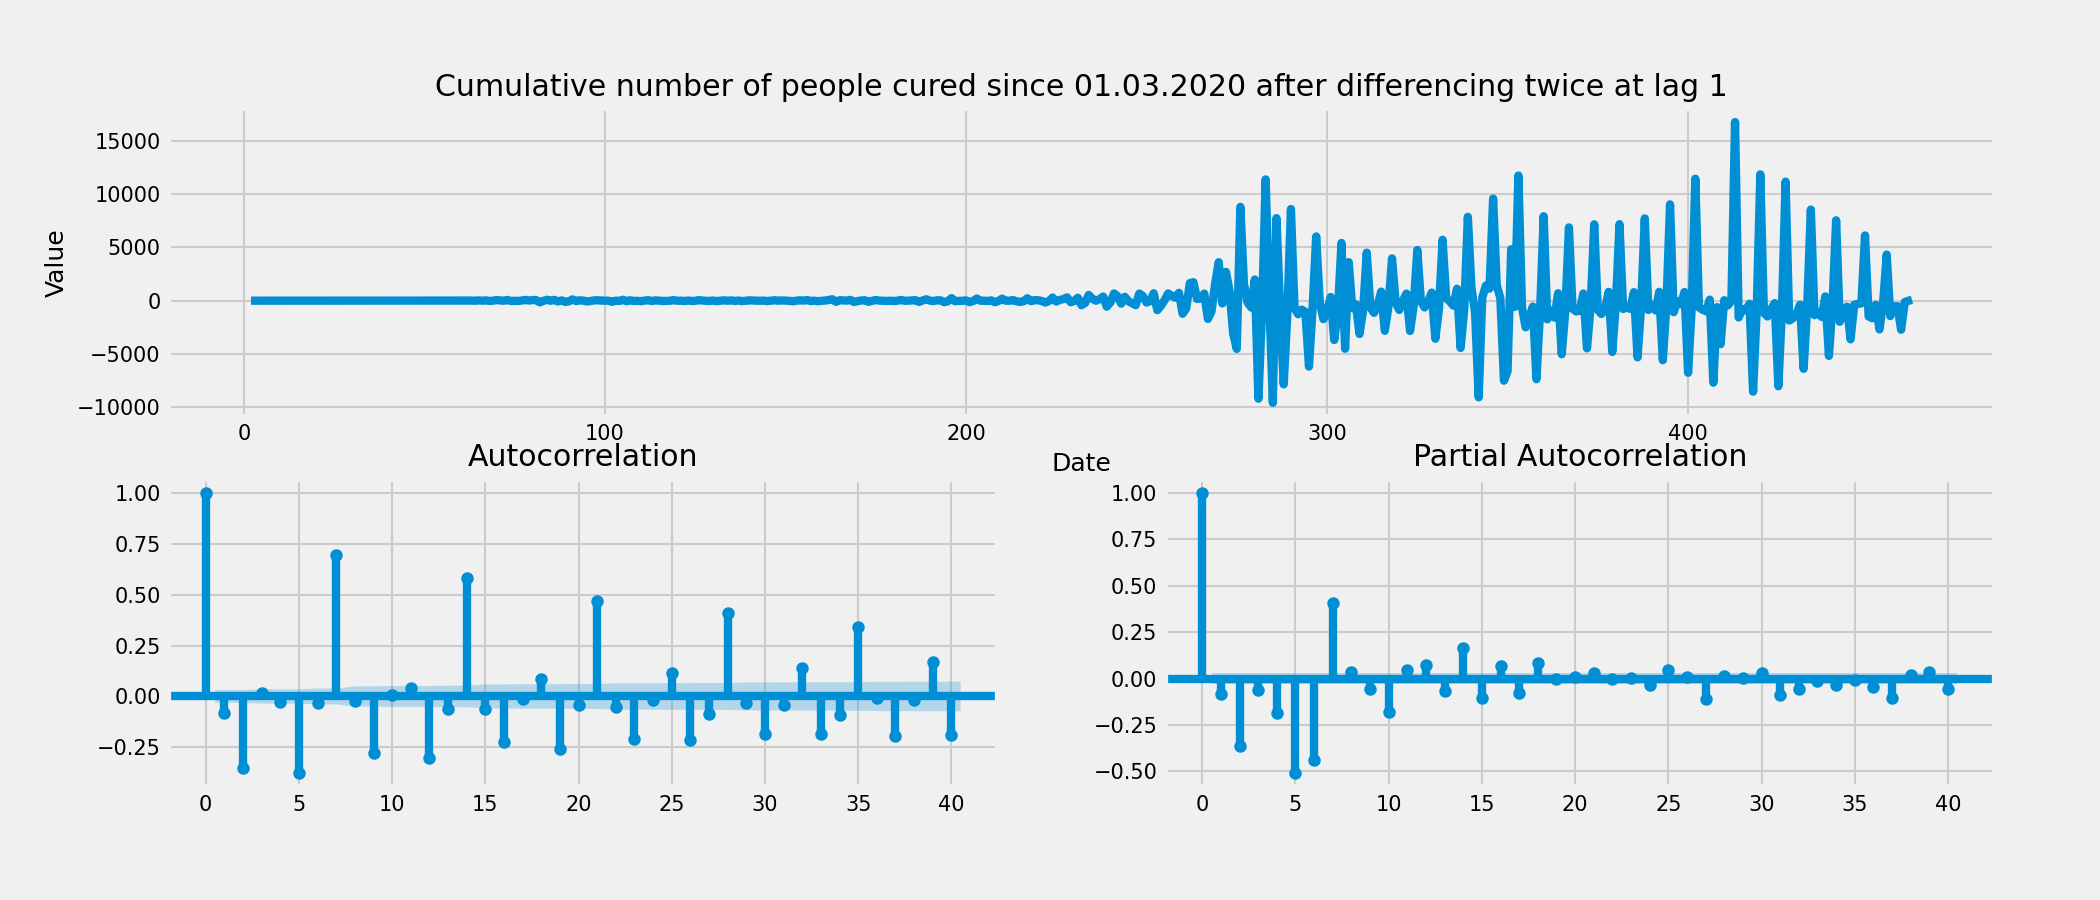
\includegraphics[width=1\textwidth, height=0.28\textwidth]{figures/chapter_04/cured_ts/ts_diff1_1_cured.png}
  \label{fig:cured_diff_1_1}} \\
  \subfloat[d][The cumulative number of people cured time series after differencing at lag 1 and 7.]{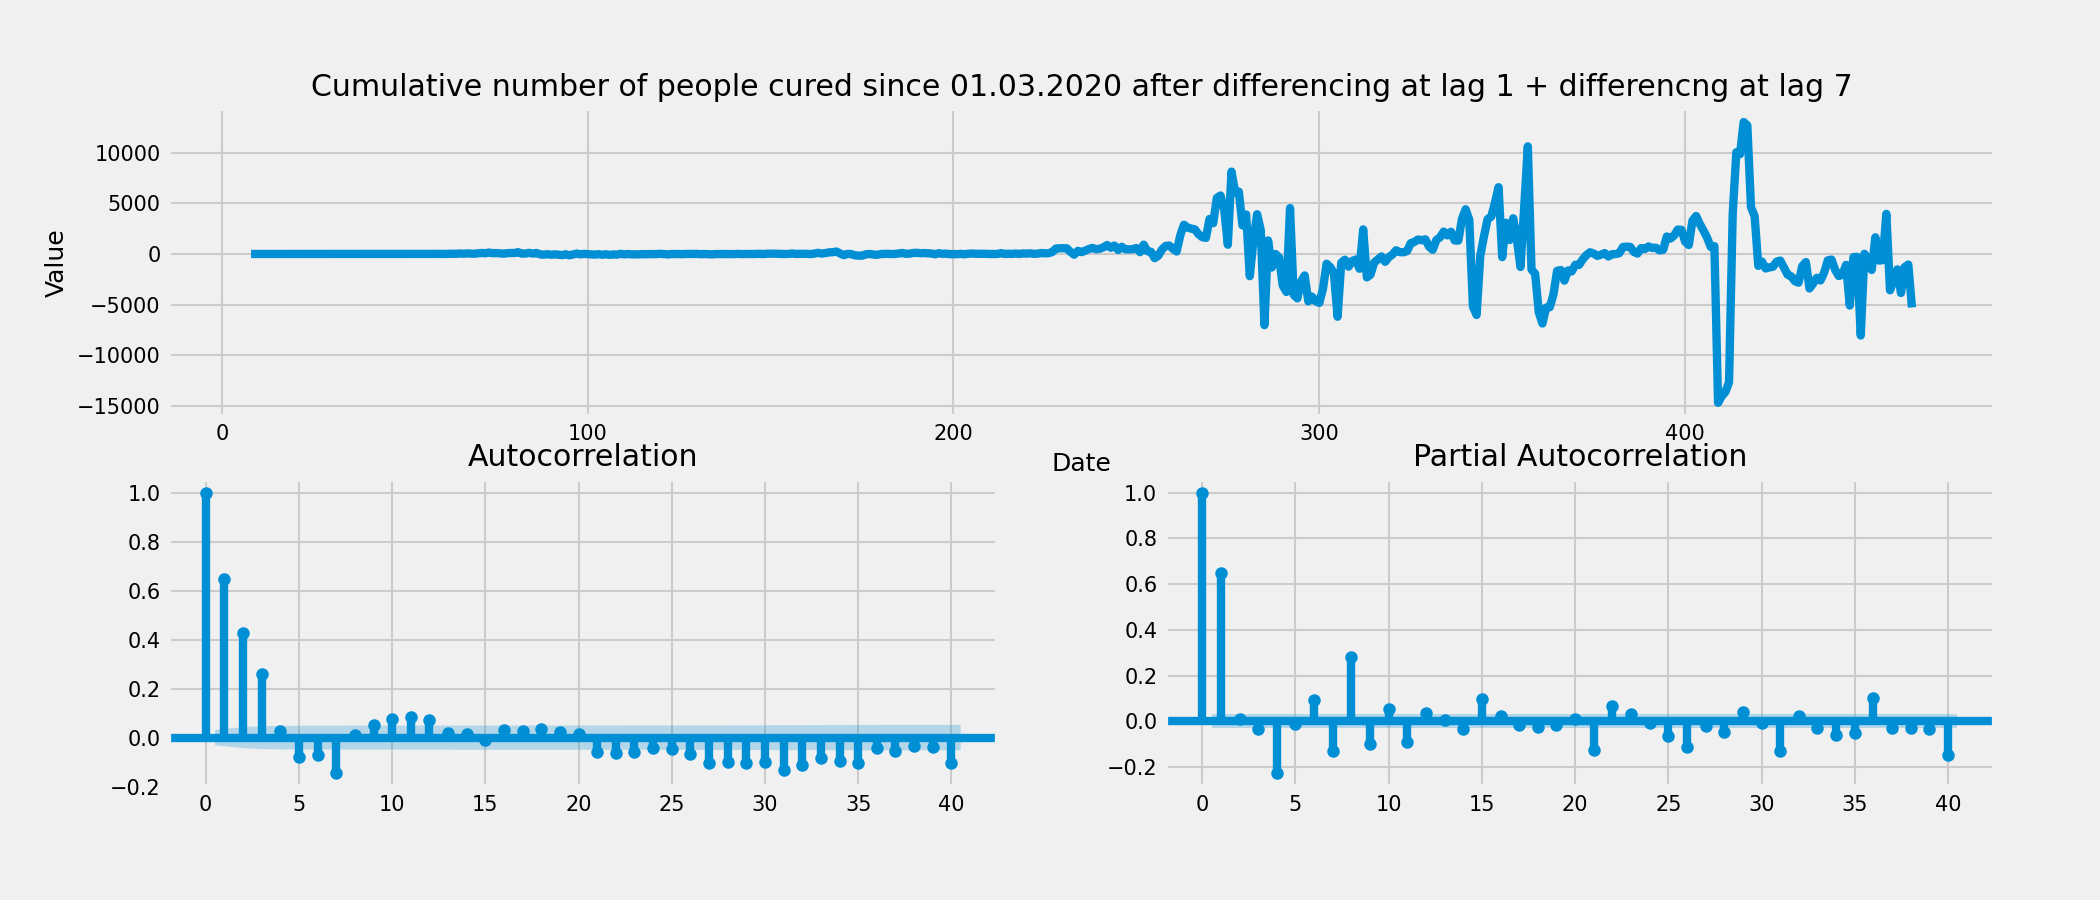
\includegraphics[width=1\textwidth, height=0.28\textwidth]{figures/chapter_04/cured_ts/ts_diff1_7_cured.png}
  \label{fig:cured_diff_1_7}}
  \caption{The cumulative amount of people cured after different differencing sequences with the corresponding ACF and PACF.}
  \label{fig:cured_diff_ex}
\end{figure}

As in the case of the cumulative number of people infected, we can do this by one more differencing at lag 1 or lag 7 (seasonal differencing).

After the second differencing at lag 1 (Figure \ref{fig:cured_diff_1_1}), the time series is now stationary (Table \ref{tab:cured_tests_table}). There is also a considerable value of the ACF at lag 7, 14, 21 (seasonality). This fact indicates that the potential order of the seasonal autoregressive part is 1.

After differencing at lag 7 (Figure \ref{fig:cured_diff_1_7}), the time series is now also stationary (Table \ref{tab:cured_tests_table}). We got rid of seasonality. The ACF shows a fast decrease, and the PACF shows a drop after the first lag, so we can say that the order of the general autoregressive component can be equal to 1. 

Based on the above, the cumulative number of people cured time series is possibly generated by the process that can be described by SARIMA(1, 2, 0) $\times$ (1, 0, 0$)_7$ or SARIMA(1, 1, 0) $\times$ (1, 1, 0$)_7$ models.

\subsection{Cumulative number of people dead time series}

Originally, the third selected time series is also a cumulative sum. After the first differencing at lag 1, it is clear that it still has the global trend, but no seasonality at all. 

Figure \ref{fig:dead_diff} demonstrates that after the second difference at lag 1, we got rid of the global trend. 

It is clear that there are no interesting phenomena in the data until the beginning of June (we can get rid of these measurements in the future). This period is also fundamentally different from the rest of the time series.

\begin{table}[!ht]
    \centering
    \begin{tabular}{|p{3cm}||p{3cm}| p{3cm}|}
    \hline
    Time series & Dikey-Fuller test p-value & KPSS test p-value\\
    \hline
    Original time series& 0.951460 & 0.010000\\
	\hline
	1x at lag 1 & 0.229294 & 0.010000\\
	\hline
	2x at lag 1 &  0.003183 & 0.030002\\
	\hline
	2x at lag 1 + Box-Cox &  0.035768 & 0.100000\\
	\hline
	2x at lag 1 + drop &  0.021909 & 0.061904\\
 \hline
\end{tabular}
    \caption{The Cumulative number of people dead: results of the stationarity tests.}
    \label{tab:dead_tests_table}
\end{table}

The ACF and PACF contain the drop after lag 1. It can indicate the absence of the autoregressive component, but the moving average order can be equal to 1. However, stationarity tests both reject the null hypothesis (Table \ref{tab:dead_tests_table}). It means that the data are likely heteroscedastic and may have structural changes over time.

\begin{figure}[!htb]
  \centering
  \subfloat[a][The original cumulative number of people dead time series.]{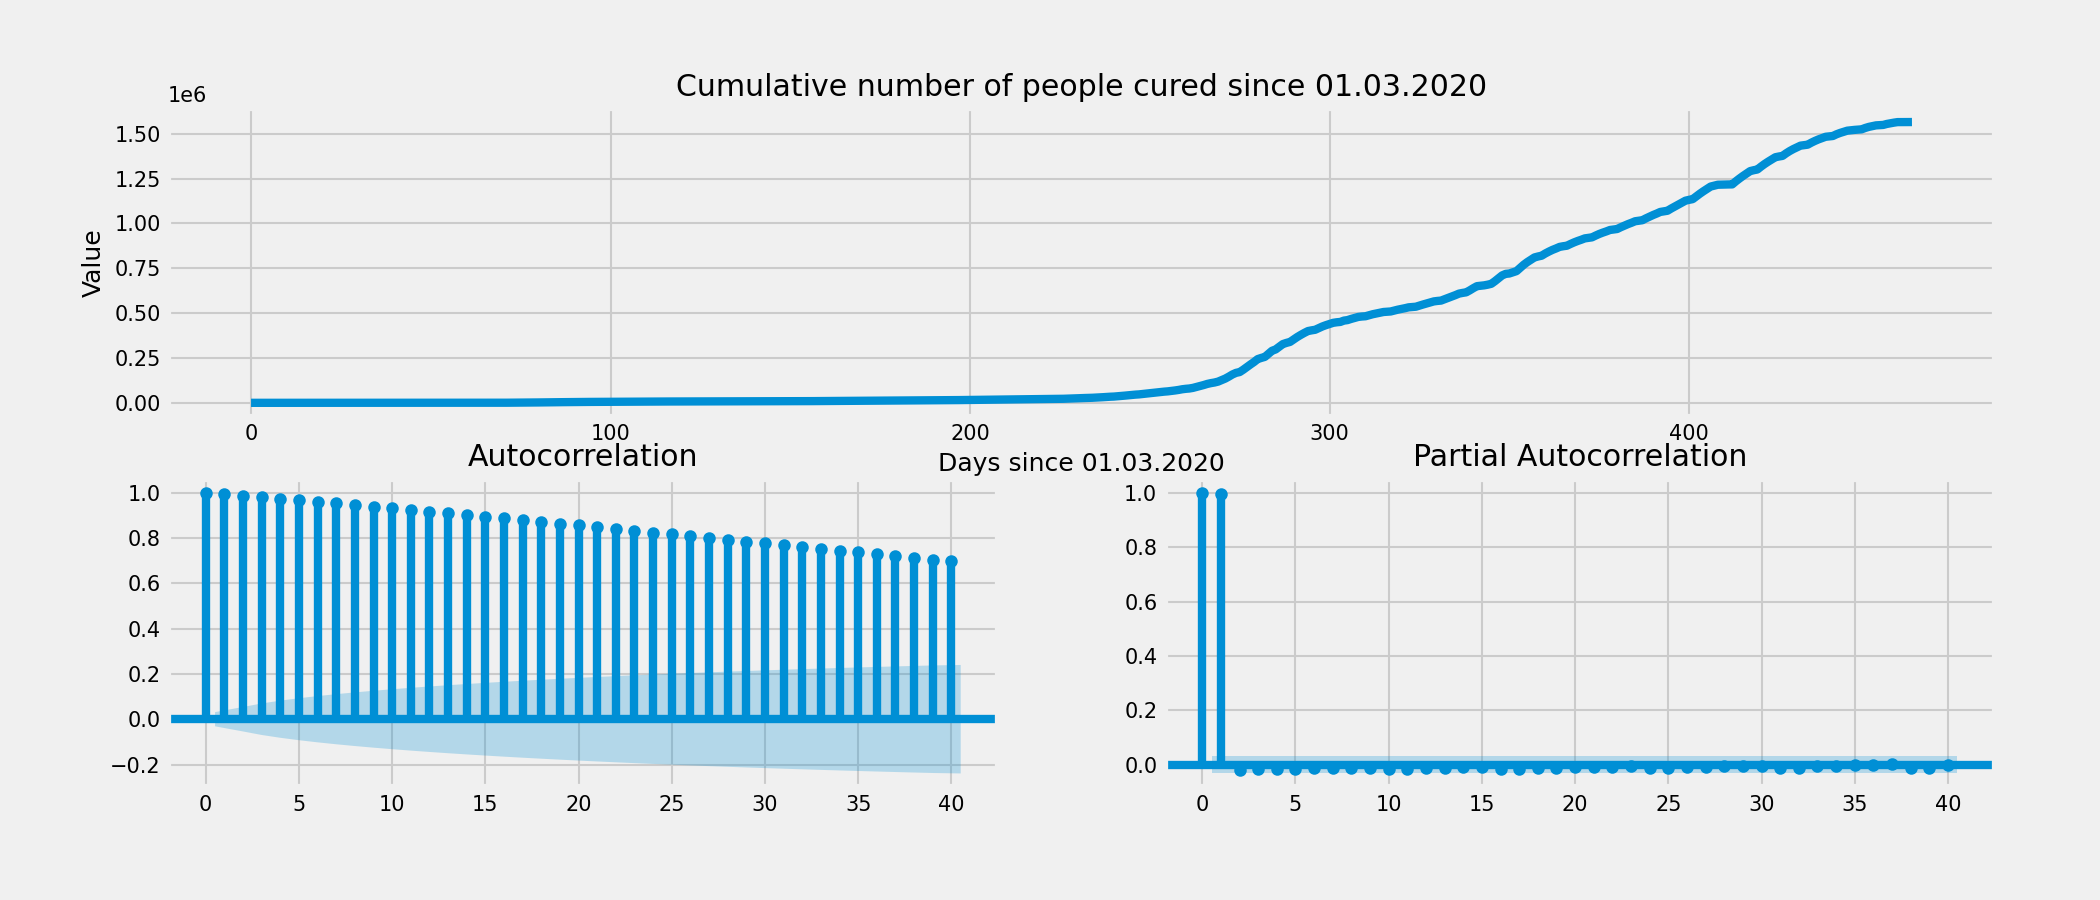
\includegraphics[width=1\textwidth, height=0.3\textwidth]{figures/chapter_04/original_ts/ts_orig_cured.png}
  \label{fig:orig_dead}} \\
  \subfloat[b][The cumulative number of people dead time series after differencing at lag 1.]{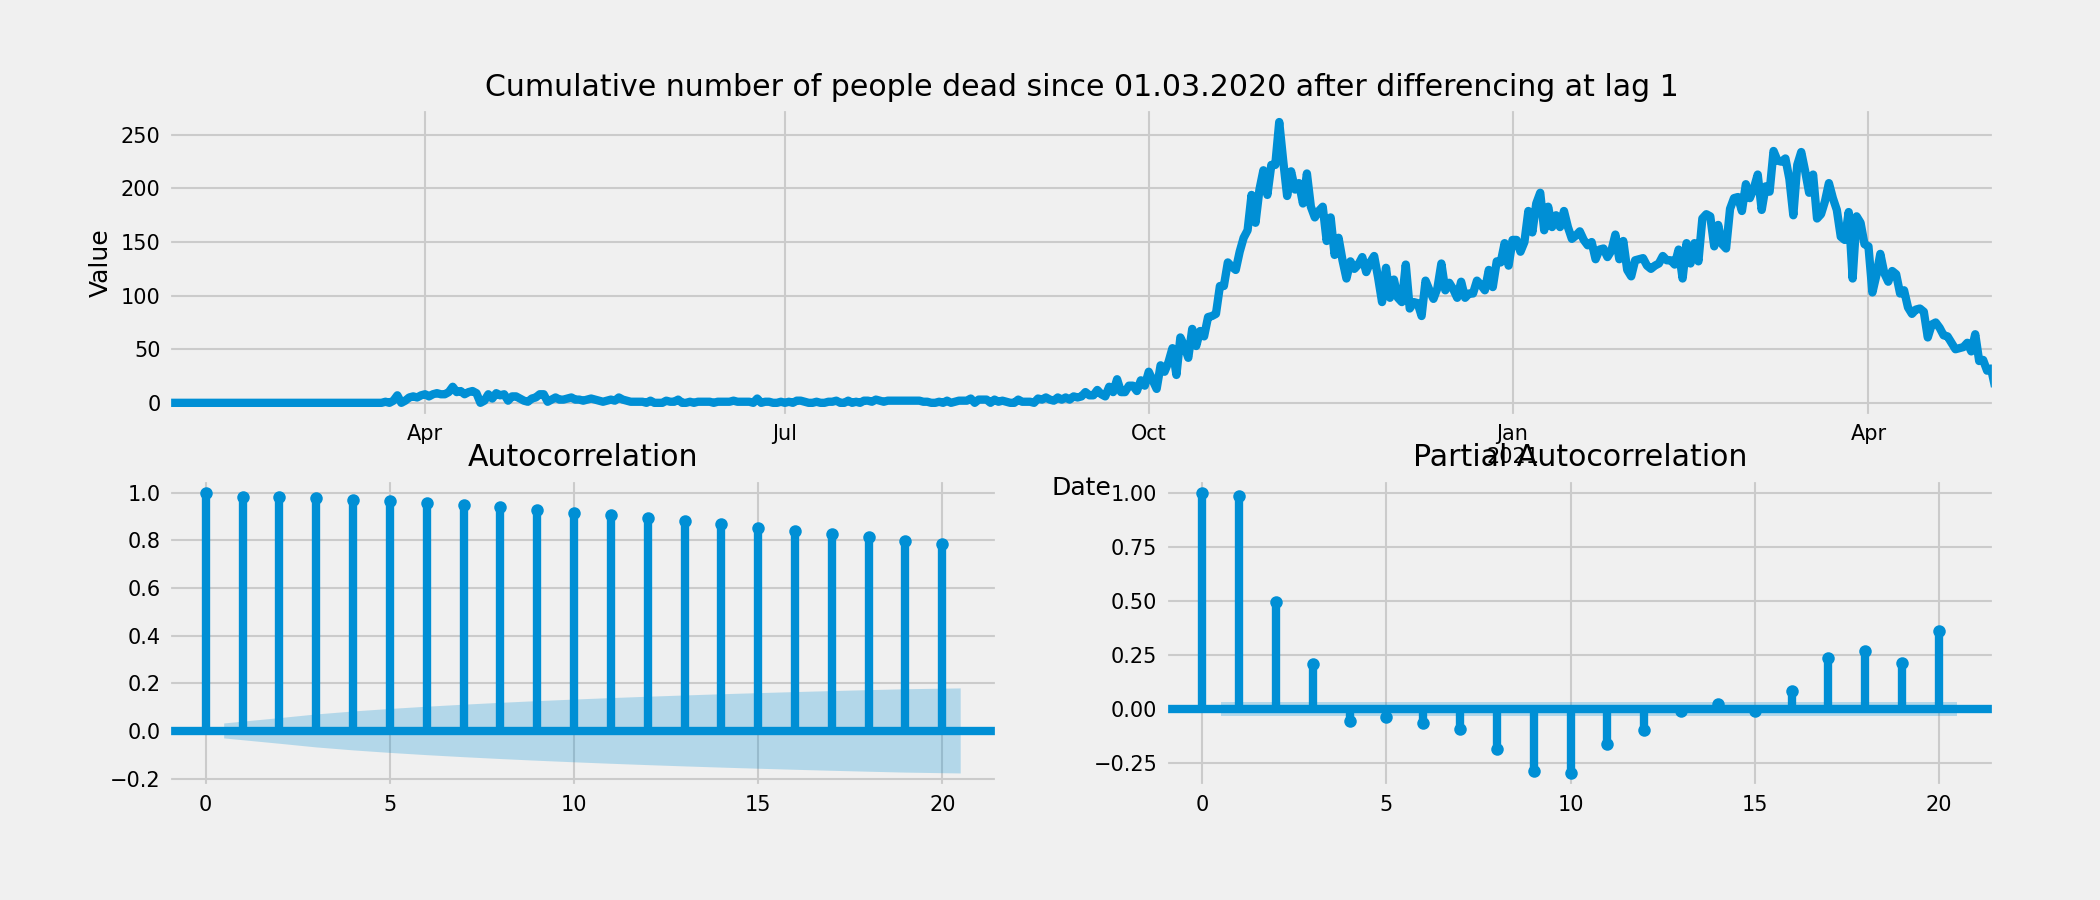
\includegraphics[width=1\textwidth, height=0.3\textwidth]{figures/chapter_04/dead_ts/ts_diff_dead.png}
  \label{fig:dead_diff}} \\
  \subfloat[c][The cumulative number of people dead time series after double differencing at lag 1.]{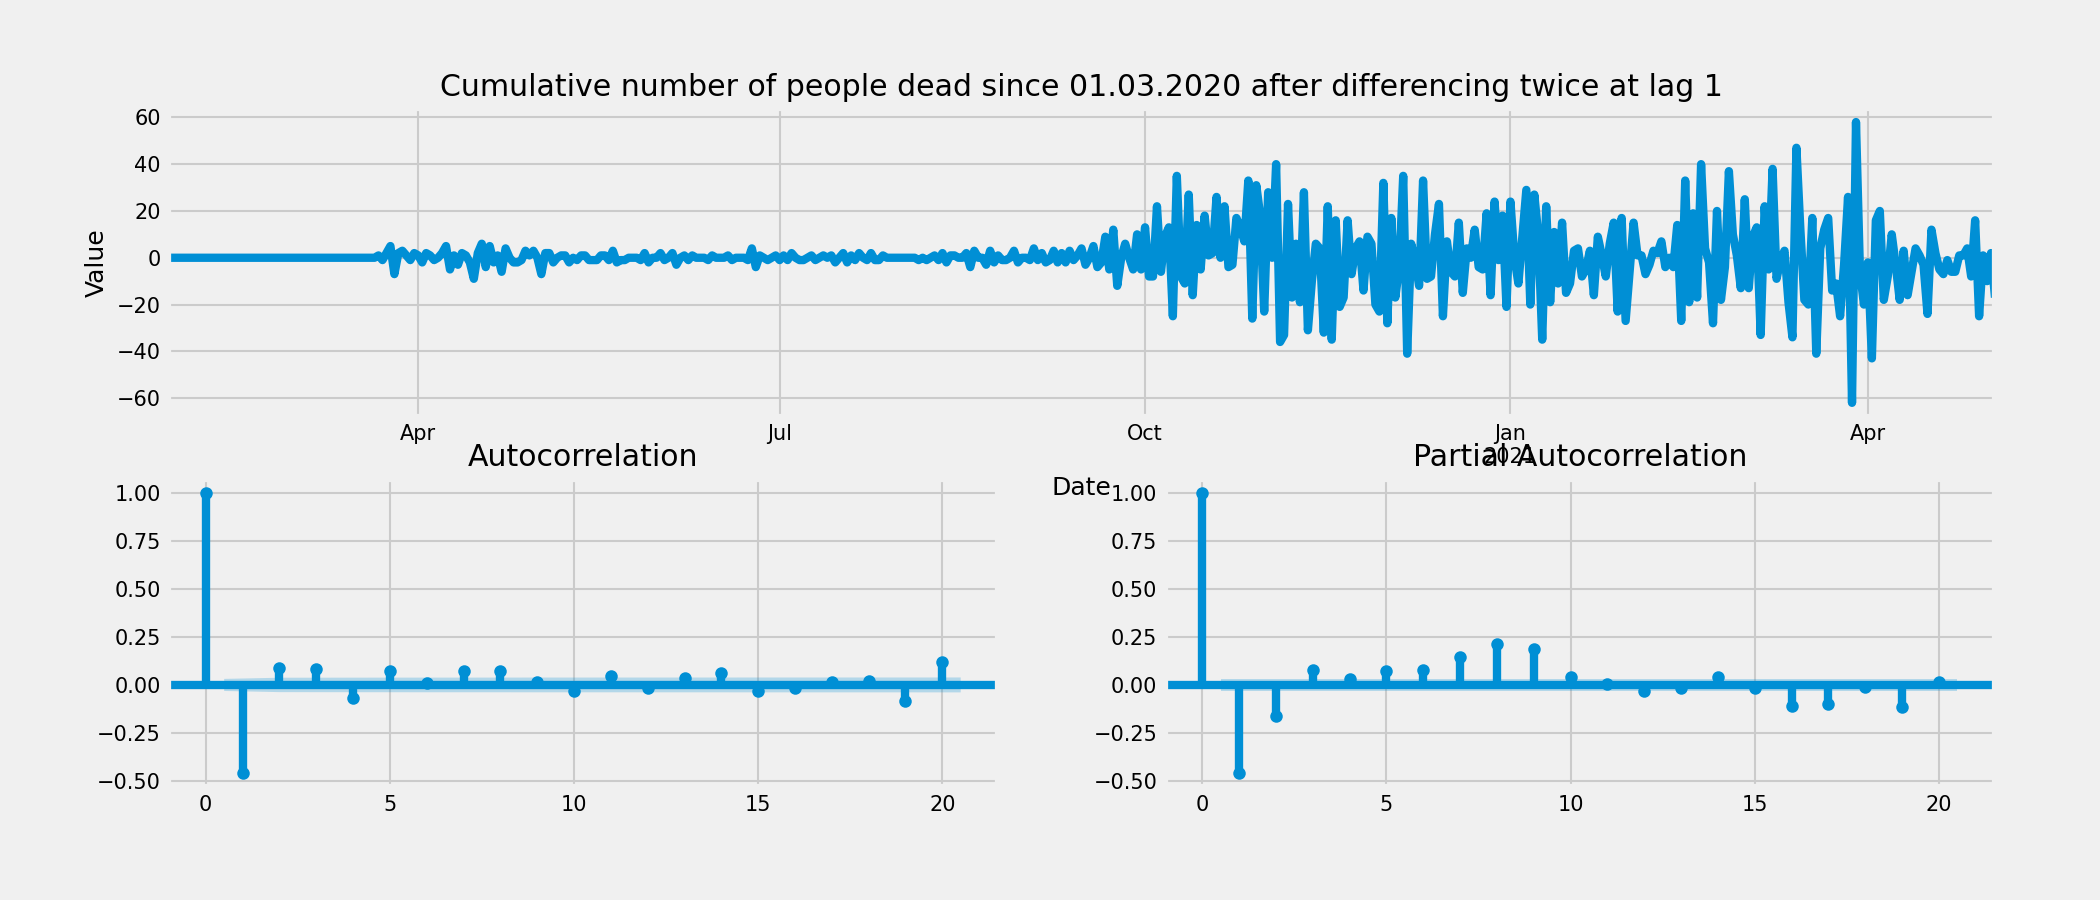
\includegraphics[width=1\textwidth, height=0.3\textwidth]{figures/chapter_04/dead_ts/ts_diff1_1_dead.png}
  \label{fig:dead_diff_1_1}} \\
  \caption{The cumulative amount of people cured after different differencing sequences with the corresponding ACF and PACF.}
  \label{fig:dead_diff_ex}
\end{figure}
It is possible to reduce the heteroscedasticity in the data by application of, for example, Box-Cox or logarithmic transformations (according to their properties) or by dropping all measurements until June 1, 2020.

Table \ref{tab:dead_tests_table} shows that after at least one of these manipulations, the tests indicate the stationarity of the time series.

Now we can say that the cumulative number of people dead time series potentially can be modeled using ARIMA(0, 2, 1) model.

\begin{figure}[!htb]
  \centering
  \subfloat[a][The number of active cases time series]{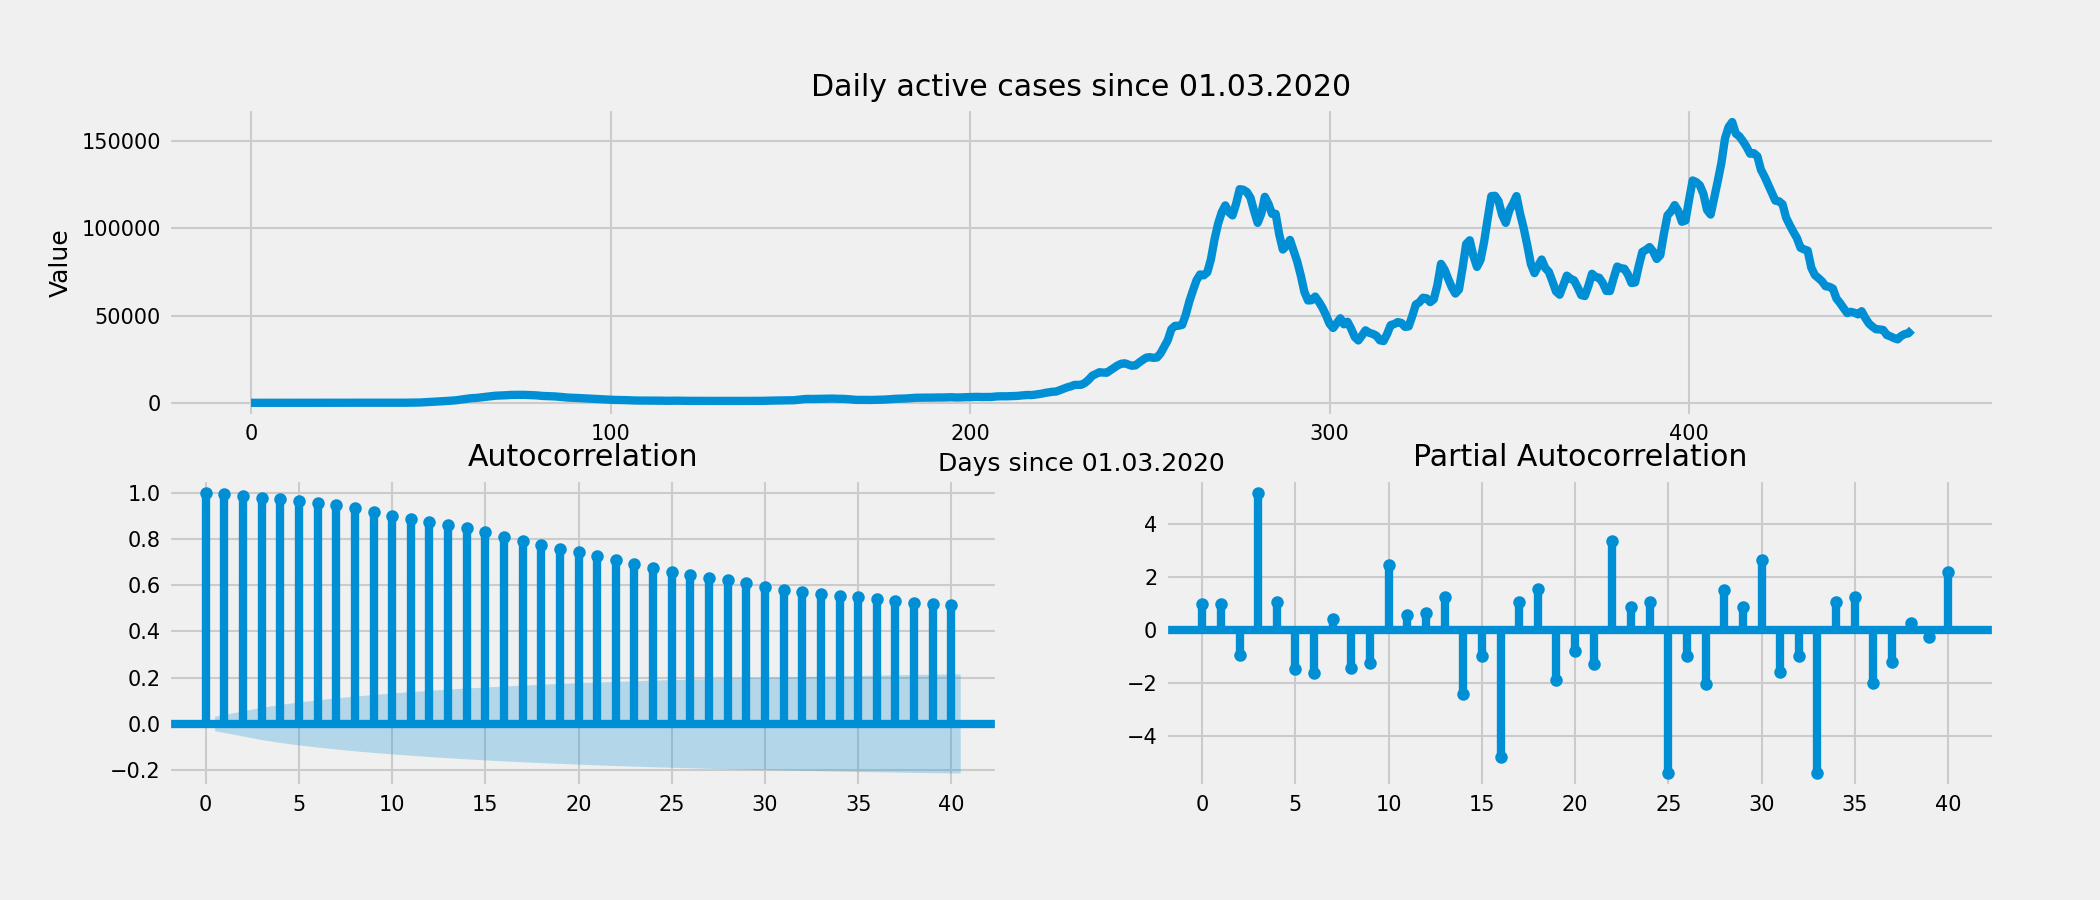
\includegraphics[width=1\textwidth, height=0.28\textwidth]{figures/chapter_04/original_ts/ts_orig_iactive.png}
  \label{fig:orig_active}} \\
  \subfloat[b][The number of active cases time series after differencing at lag 1.]{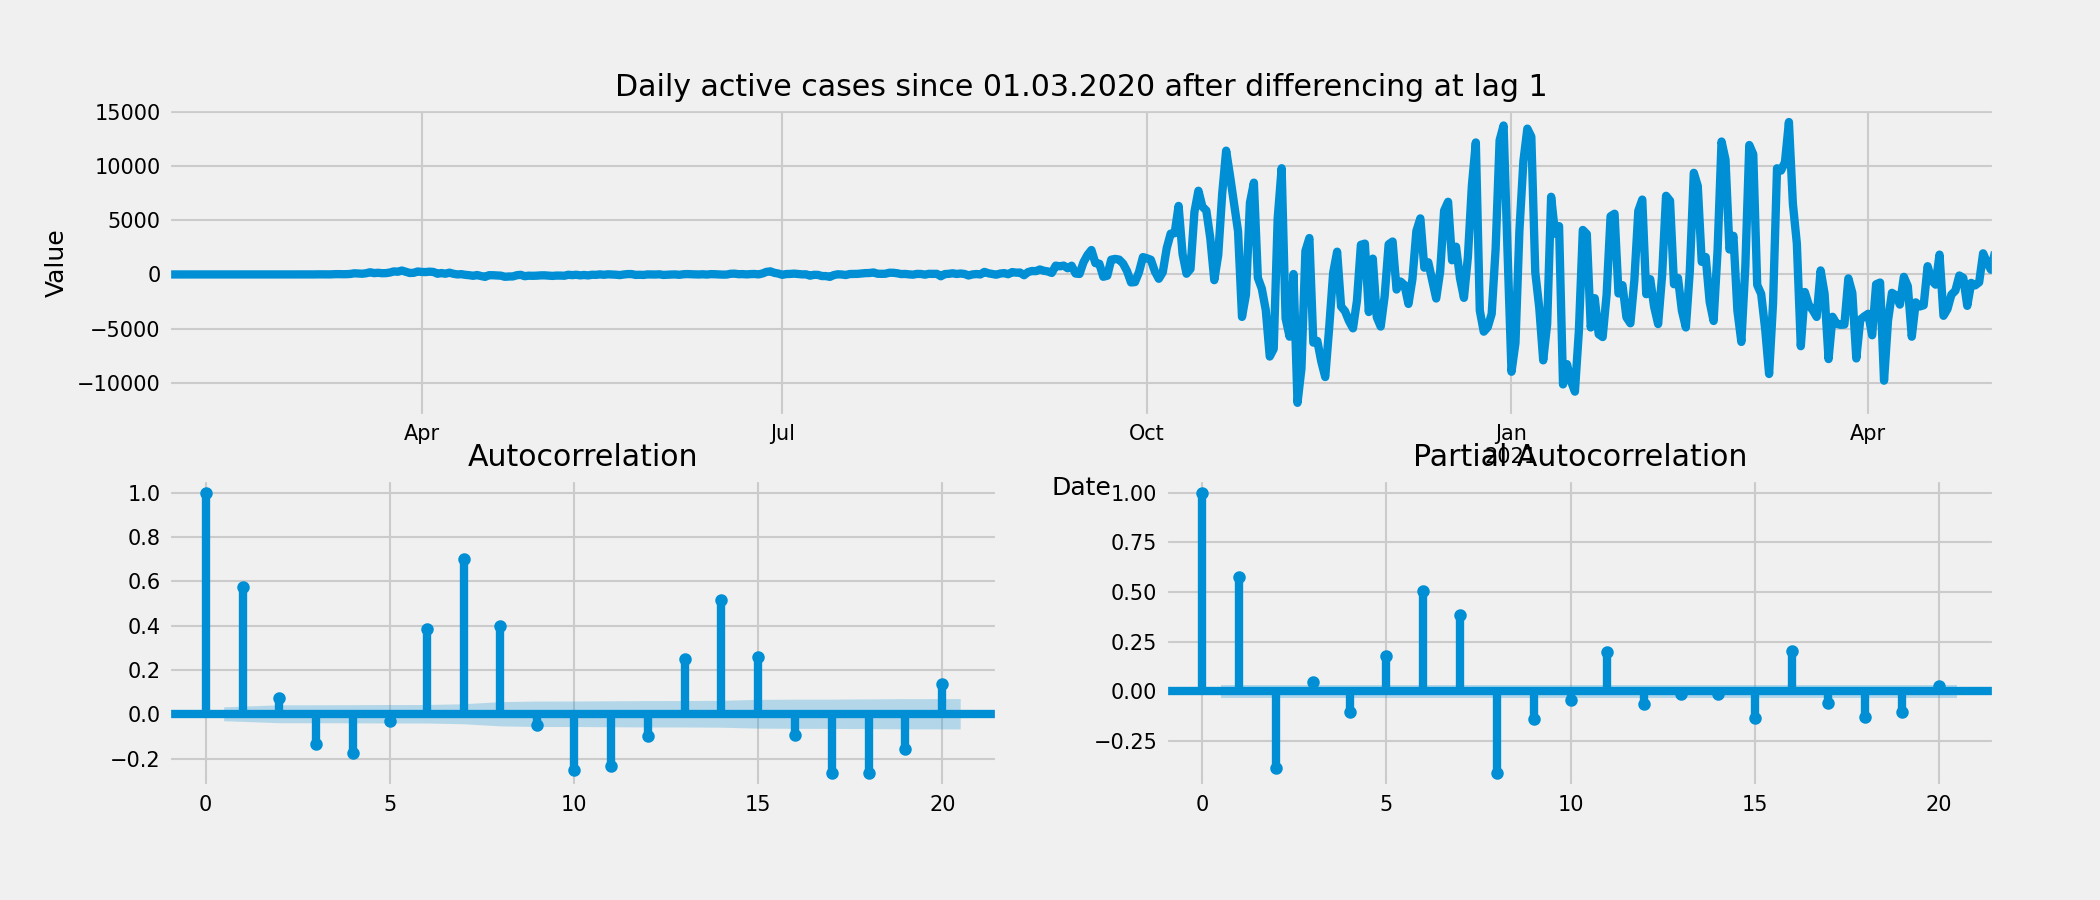
\includegraphics[width=1\textwidth, height=0.28\textwidth]{figures/chapter_04/active_ts/ts_diff_active.png}
  \label{fig:active_diff}} \\
  \subfloat[c][The number of active cases time series after differencing at lag 1 and lag 7.]{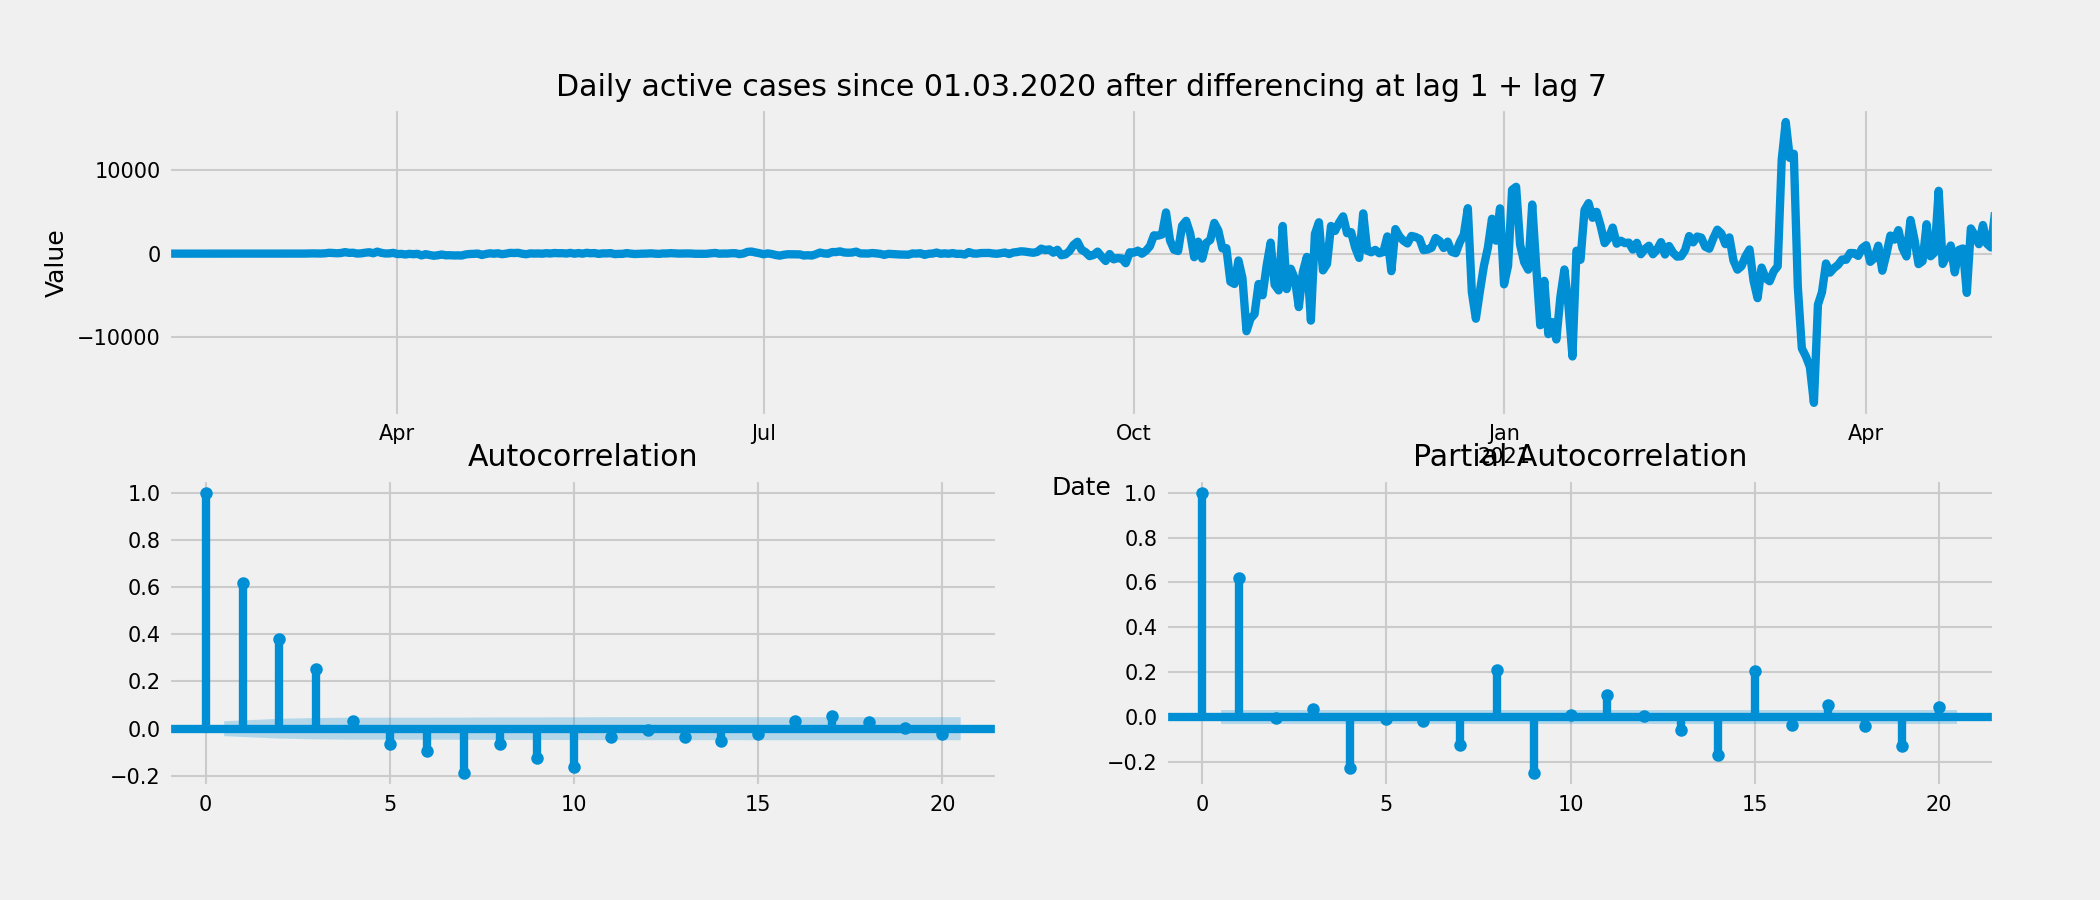
\includegraphics[width=1\textwidth, height=0.28\textwidth]{figures/chapter_04/active_ts/ts_diff1_7_active.png}
  \label{fig:active_diff_1_7}} \\
  \caption{The number of active cases time series after different differencing sequences with the corresponding ACF and PACF.}
  \label{fig:active_diff_ex}
\end{figure}

\subsection{The number of active cases time series}

The fourth selected time series describes the number of active cases. In Figure \ref{fig:orig_active} you can see it before any manipulation. It has a global trend, but we can say anything about the seasonal patterns or about the order of autoregressive and moving average components. Similar to the other time series, the period until June 1, 2020, is fundamentally different and does not contain any useful information. Stationarity testing (Table \ref{tab:active_tests_table}) indicates that the the time series is nonstationary. Thus, we need to perform differencing at lag 1.

Figure \ref{fig:active_diff} shows that after the first differencing we got rid of the global trend, plus it is now clear that there is a seasonal pattern with weekly periodicity. The ACF and PACF show that the order of the seasonal autoregressive component is equal to 1 (significant correlation at lags 7, 14, and so on). According to the tests, the time series is now stationary. However, it is difficult to determine the order of the general autoregressive or moving average component. 

After differencing at lag 7 (to remove seasonality), it is visible that the order of the general autoregressive component is equal to 1 (the value of the ACF slowly decreases, the value of the PACF drops after lag 1).

\begin{table}[!ht]
    \centering
    \begin{tabular}{|p{3cm}||p{3cm}| p{3cm}|}
    \hline
    Time series & Dikey-Fuller test p-value & KPSS test p-value\\
    \hline
    Original time series& 0.290402 & 0.017614\\
	\hline
	1x at lag 1 & 0.000158 & 0.100000\\
	\hline
	1x at lag 1; 1x at lag 7 &  0.000005 & 0.100000\\
	\hline
\end{tabular}
    \caption{The number of active cases: results of the stationarity tests.}
    \label{tab:active_tests_table}
\end{table}

To summarize, this time series can be modeled using the SARIMA(1, 1, 0) $\times$ (1, 0, 0$)_7$ or SARIMA(1, 1, 0) $\times$ (1, 1, 0$)_7$ models.

\hypertarget{s3.3}{\section{Facebook Prophet modeling}}

After applying the basic analysis, the selected time series are ready for modeling using the Facebook Prophet model. 

In this section, the more detailed pipeline has been formulated as
\begin{enumerate}
    \item find the best configuration of all 3 defined components (trend, seasonal, holidays) for each selected time series.
    \item perform hyperparameters tuning using the cross-validation.
    \item evaluate the model using specified metrics.
    \item obtain a set of changepoints for each time series individually, evaluate the possibility of using a single shared set for all selected time series.
    \item create a custom set of changepoints based on the public information about restrictions provided by the Czech government and compare it with automatically detected
    \item perform the forecasts
    \item find some correlations between government restrictions and changes in the growth rate of the selected time series.
\end{enumerate}

As we found out in the section of time series analysis, all selected time series have a part significantly distinct from the remaining time series (for example, until June 1, 2020), where nothing special happens. We can ignore this data during the future modeling (because this period has no information about the evolution of the COVID-19 pandemic since the first wave). However, the Facebook Prophet model supports the global trend growth changes, so it will be enough to drop the period with the target variable equal to 0.

\subsection{Parameter estimation mechanism}

According to the specified pipeline, the first step is to perform hyperparameter tuning using the time series cross-validation technique. 

We need to define the parameters of the cross-validation. It is also necessary to specify the parameters of the model used during the cross-validation that will can set manually. We will use the knowledge received during the basic time series analysis and the information from the official Facebook Prophet documentation \cite{ProphetDoc}.

The cross-validation parameters are: 
\begin{itemize}
    \item initial cutoff $=$ 150 days ($\sim$ July 1, 2020, covers the beginning of the useful data),
    \item forecast horizon $=$ 14 days (this value was selected because it is equal to 2 $\times$ length of the seasonal pattern and can be potentially useful during the pandemic analysis).
\end{itemize}

The manually specified parameters of the model are \textit{set of holidays} and \textit{seasonality} (for seasonal time series).

The set of holidays is specified using the inbuilt method of the Prophet model that adds a list of national holidays (depends on the country).

Table \ref{tab:holidays_set} demonstrates the curtain list of holidays specified for the Czech Republic.

\begin{table}[!ht]
    \centering
    \begin{tabular}{|p{1cm}||p{8cm}|}
    \hline
    Index & Holiday name\\
    \hline
    0 & Day of the Restoration of the Independent Czech State \\
    \hline
    1 & Good Friday\\
    \hline
    2 & Easter Monday\\
    \hline
    3 & Labor Day\\
    \hline
    4 & Victory Day\\
    \hline
    5 & Day of the Slavic heralds Cyril and Methodius\\
    \hline
    6 & Day of the burning of master Jan Hus\\
    \hline
    7 & Czech Statehood Day\\
    \hline
    8 & Day of the establishment of an independent Czechoslovak state\\
    \hline
    9 & Day of the Struggle for Freedom and Democracy\\
    \hline
    10 & Christmas Eve\\
    \hline
    11 & 1st Christmas holiday\\
    \hline
    12 & 2nd Christmas holiday\\
    \hline
\end{tabular}
    \caption{The set of holidays used in the Prophet modeling.}
    \label{tab:holidays_set}
\end{table}

For time series that contain seasonal patterns, we will also enable a \textit{weekly seasonality}. 

During the cross-validation, there is no need to compute the confidential intervals because we care only about the forecast accuracy in comparison with the historical data. 

We also will cut the last 14 days off to evaluate model performance on the unseen data.

\subsubsection{Data transformation before modeling}

For the Prophet modeling, we decided to drop the first 55 days (until the day of the first death) to get rid of measures with zero value and remain equal length of the selected time series.

\subsubsection{Cross-validation accuracy metrics}

For evaluation of the cross-validation results, we decided to use MAPE metric supported by the cross-validation function inside the Prophet diagnostics module \cite{ProphetDoc}: 
\begin{equation}
    MAPE = \frac{100}{n}\sum_{t=1}^{n}\Big|\frac{Y_t - \hat{Y_t}}{Y_t}\Big|,
\end{equation}    
where $n$ is an amount of forecasted points, $Y_t$ is the real value of the observed variable $Y$ at timestamp $t$, and $\hat{Y_t}$ is the forecasted value at timestamp $t$.

As we noticed earlier in Chapter \hyperlink{ch3}{3}, the resulting error is computed as the mean of the errors obtained from all forecasts made during the cross-validation process.  

According to the fact that we have selected 4 different time series, we will perform 4 different cross-validations.

Table \ref{tab:cross_val_grid} contains information about the parameters to tune.

\begin{table}[!ht]
    \centering
    \begin{tabular}{|p{6cm}||p{4cm}|}
    \hline
    Parameter name & Possible values\\
    \hline
    \verb|changepoint_prior_scale| & 0.1, 0.5, 0.8, 1.0\\
    \hline
    \verb|seasonality_prior_scale| & 0.1, 1.0, 10.0\\
    \hline
    \verb|seasonality_mode| & multiplicative, additive\\
    \hline
    \verb|holidays_prior_scale| & 0.1, 1.0, 10.0\\
    \hline
    \verb|changepoint_range| & 0.8, 0.9, 0.95\\
    \hline
\end{tabular}
    \caption{The Prophet cross-validation parameter grid.}
    \label{tab:cross_val_grid}
\end{table}

The \verb|changepoint_prior_scale| parameter corresponds to the parameter $\tau$ of the Laplace distribution (Section \ref{sec:automatic_cp_detection}). It controls the growth rate change flexibility. The \verb|seasonality_prior_scale| parameter (for seasonal time series )regulates strength of the seasonal model. According to the official Prophet documentation \cite{ProphetDoc}, larger values allow larger seasonal fluctuations, smaller values mitigate the seasonality. The \verb|seasonality_mode| parameter specifies a type of seasonal model (multiplier or addendum). The \verb|holidays_prior_scale| parameter controls the sensitivity to the changes caused by holidays. The \verb|changepoint_range| parameter defines the percentage of the time series (from the beginning) within which the changepoints will be distributed.

\subsubsection{Cross-validation results}

Table \ref{tab:cross_val_res} contains information about the best performance parameters for each model.

\begin{table}[!ht]
\catcode`\-=12
\centering
\resizebox{\textwidth}{!}{%
\begin{tabular}{|l|l|l|l|}
\hline
 &
  \multicolumn{2}{l|}{\textit{\textbf{Parameter}}} &
  \textit{\textbf{Error}} \\ \hline
\textbf{Time series} &
  \textbf{Name} &
  \textbf{Value} &
  \textbf{MAPE (\%)} \\ \hline
\multirow{5}{*}{\begin{tabular}[c]{@{}l@{}}Cumulative number \\ of people infected\end{tabular}} &
  changepoint\_prior\_scale &
  0.8 &
  \multirow{5}{*}{5.314} \\ \cline{2-3}
 & seasonality\_prior\_scale & 10.0  &  \\ \cline{2-3}
 & seasonality\_mode         & 10.0 &  \\ \cline{2-3}
 & holidays\_prior\_scale    & additive &  \\ \cline{2-3}
 & changepoint\_range        & 0.95 &  \\ \hline
\multirow{5}{*}{\begin{tabular}[c]{@{}l@{}}Cumulative number \\ of people cured\end{tabular}} &
  changepoint\_prior\_scale &
  1.0 &
  \multirow{5}{*}{5.381} \\ \cline{2-3}
 & seasonality\_prior\_scale & 1.0 &  \\ \cline{2-3}
 & seasonality\_mode         & additive &  \\ \cline{2-3}
 & holidays\_prior\_scale    & 10.0 &  \\ \cline{2-3}
 & changepoint\_range        & 0.95  &  \\ \hline
\multirow{3}{*}{\begin{tabular}[c]{@{}l@{}}Cumulative number \\ of people dead\end{tabular}} &
  changepoint\_prior\_scale &
  1.0 &
  \multirow{3}{*}{5.111} \\ \cline{2-3}
 & holidays\_prior\_scale    & 1.0  &  \\ \cline{2-3}
 & changepoint\_range        & 0.95 &  \\ \hline
\multirow{5}{*}{\begin{tabular}[c]{@{}l@{}}Number of active \\ cases\end{tabular}} &
  changepoint\_prior\_scale &
  1.0 &
  \multirow{5}{*}{28.957} \\ \cline{2-3}
 & seasonality\_prior\_scale & 10.0  &  \\ \cline{2-3}
 & seasonality\_mode         & mult. &  \\ \cline{2-3}
 & holidays\_prior\_scale    & 0.1 &  \\ \cline{2-3}
 & changepoint\_range        & 0.95 &  \\ \hline
\end{tabular}%
}
\caption{The best set of the hyperparameters for each time series.}
\label{tab:cross_val_res}
\end{table}

It is visible that the cross-validation results are relatively satisfactory. Average MAPE varies between 5-28\%. 

The number of active cases time series has a larger average MAPE because it has more expressive growth changes (other time series contain a cumulative sum, this time series contains information about daily active cases). It means that, on average, the data before and after cutoffs have more distinct differences in trend directions. It can potentially affect the future forecast of the unseen data. To reduce this problem, we decided to apply \textit{the log transformation} on this time series (according to the fact that we need to apply an inverse transform to all forecast components, we cant use Box-Cox transformation\footnote{https://github.com/facebook/prophet/issues/647 ---  Box-Cox transformation usage with Prophet problem, the inverted sum does not equal to the sum of inverted components}). 

Logarithm transformation can invert the sum in such a way that it will be equal to the product of inverted components (additive model to multiplicative, because of the logarithm). Table \ref{tab:cross_val_act_log} shows cross-validation results after this transformation. We have reduced the average MAPE from 28\% to 2.5\%. 

\begin{table}[!htb]
\catcode`\-=12
\centering
\resizebox{\textwidth}{!}{%
\begin{tabular}{|l|l|l|l|}
\hline
 &
  \multicolumn{2}{l|}{\textit{\textbf{Parameter}}} &
  \textit{\textbf{Error}} \\ \hline
\textbf{Time series} &
  \textbf{Name} &
  \textbf{Value} &
  \textbf{MAPE (\%)} \\ \hline
\multirow{5}{*}{\begin{tabular}[c]{@{}l@{}}Number of active \\ cases + log. \\ transformation\end{tabular}} &
  changepoint\_prior\_scale &
  1.0 &
  \multirow{5}{*}{2.455} \\ \cline{2-3}
 & seasonality\_prior\_scale & 10.0  &  \\ \cline{2-3}
 & holidays\_prior\_scale    & 10.0 &  \\ \cline{2-3}
 & seasonality\_mode         & additive &  \\ \cline{2-3}
 & changepoint\_range        & 0.95 &  \\ \hline
\end{tabular}%
}
\caption{The best set of the hyperparameters for the number of active cases time series after the logarithm transformation.}
\label{tab:cross_val_act_log}
\end{table}

\begin{figure}[!htb]
  \centering
  \subfloat[a][Modeled time series.]{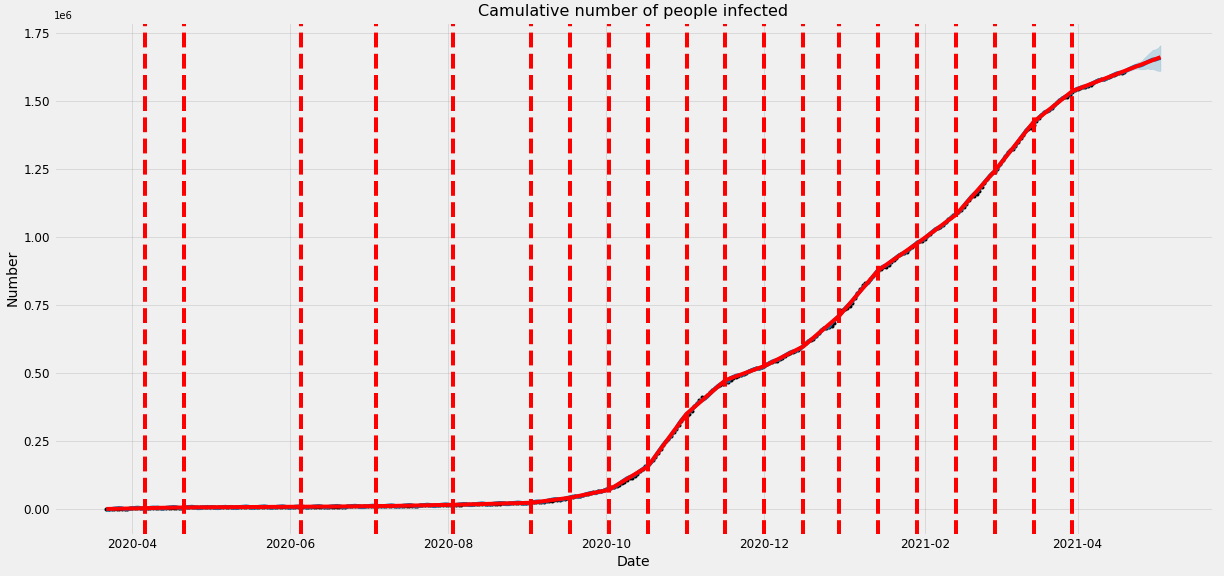
\includegraphics[width=1\textwidth, height=0.4\textwidth]{figures/chapter_04/forecast_example/infected_fbp_modeled.png}
  \label{fig:infected_modeled}} \\
  \subfloat[b][Forecast components.]{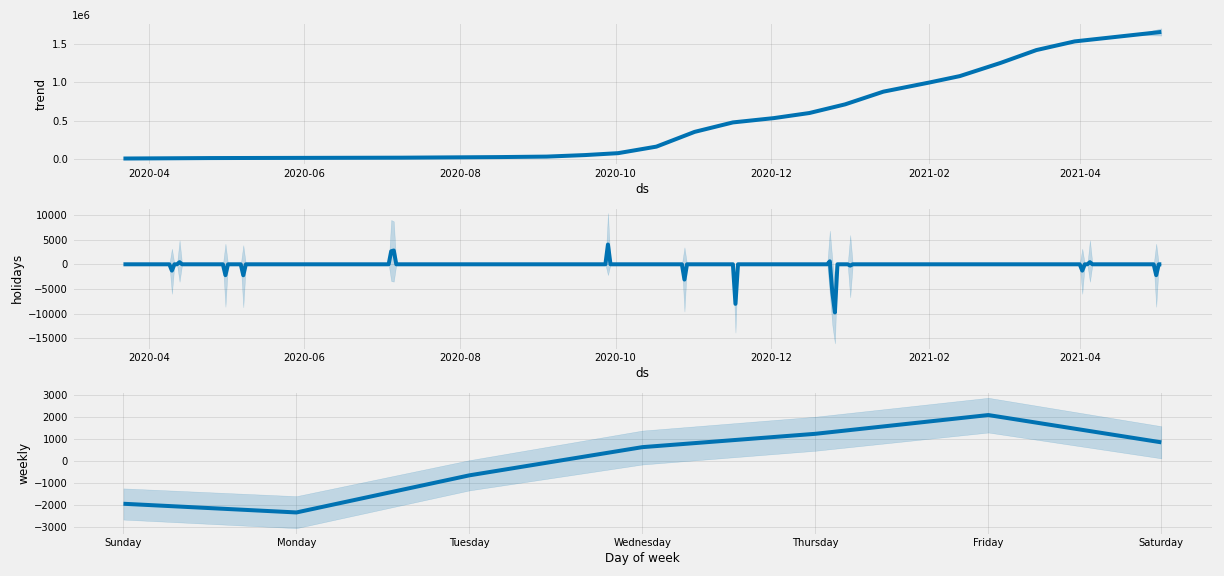
\includegraphics[width=1\textwidth, height=0.4\textwidth]{figures/chapter_04/forecast_example/infected_fbp_components.png}
  \label{fig:infected_modeled_components}} \\
  \caption{The cumulative amount of people infected modeled using the Prophet model + Forecast components.}
  \label{fig:infected_forecast_fbp}
\end{figure}

Now, we can fit new models (using tuned parameters) for each time series to analyze changepoints distribution and forecast accuracy for unseen data (the last 14 days of observations).
\hypertarget{ss332}{\subsection{Forecasting using Prophet model}}

After fitting new models to the data, it is possible to perform a forecast with 14 days forecast horizon. Figure \ref{fig:infected_forecast_fbp} shows an example of the resulting model plot with extra information about each forecast component individually. Additionally, in Figure \ref{fig:infected_forecast_last} you can see a more detailed graph with the comparison of the forecasted and the original data since the last detected changepoint (May 30, 2021) for each selected time series.

\begin{figure}[!ht]
\centering
\subfloat[a][Cumulative number of people infected time series forecast]{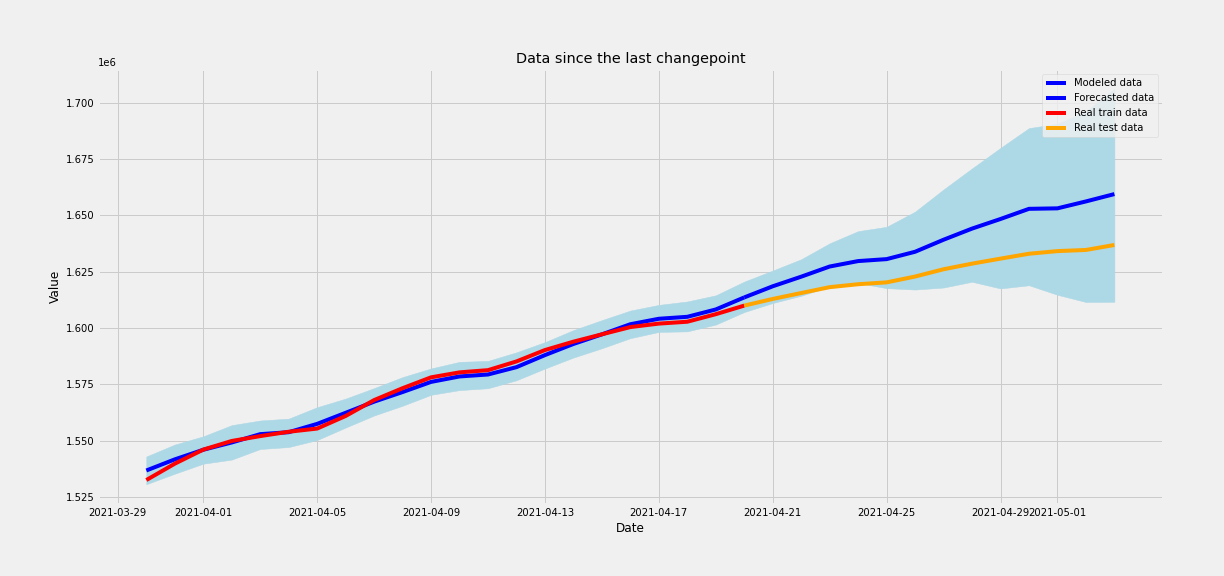
\includegraphics[width=1\textwidth, height=0.28\textwidth]{figures/chapter_04/forecast_example/forecast_infected_fc.png}\label{fig:infected_forecast_last}} \\
\subfloat[b][Cumulative number of people cured time series forecast]{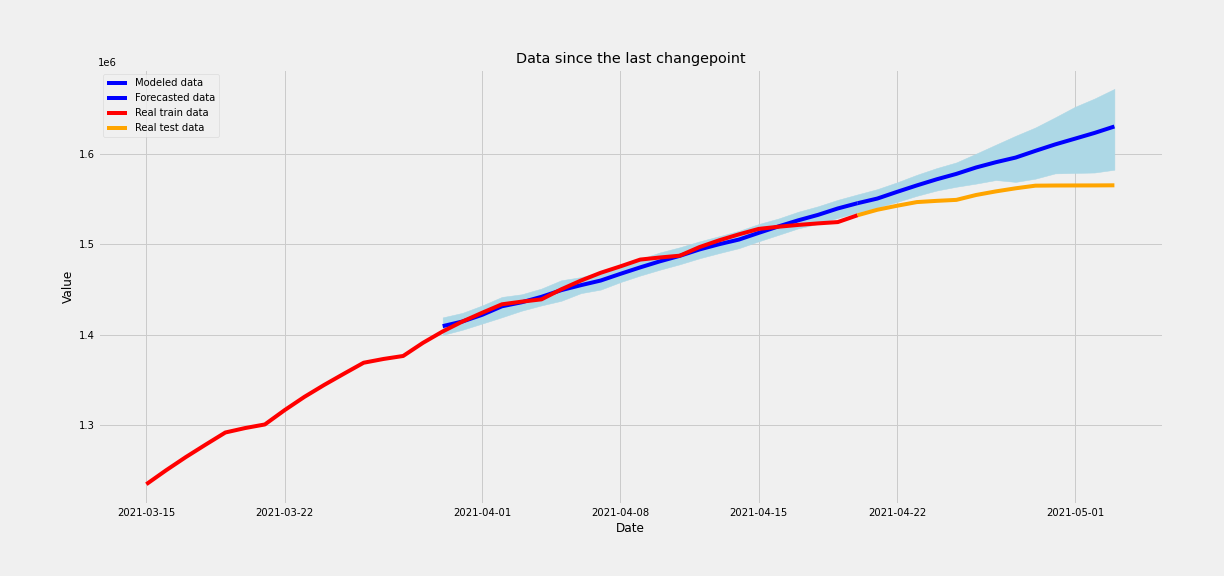
\includegraphics[width=1\textwidth, height=0.28\textwidth]{figures/chapter_04/forecast_example/forecast_cured_fc.png}\label{fig:cured_forecast_last}} \\
\subfloat[c][Cumulative number of people dead time series forecast]{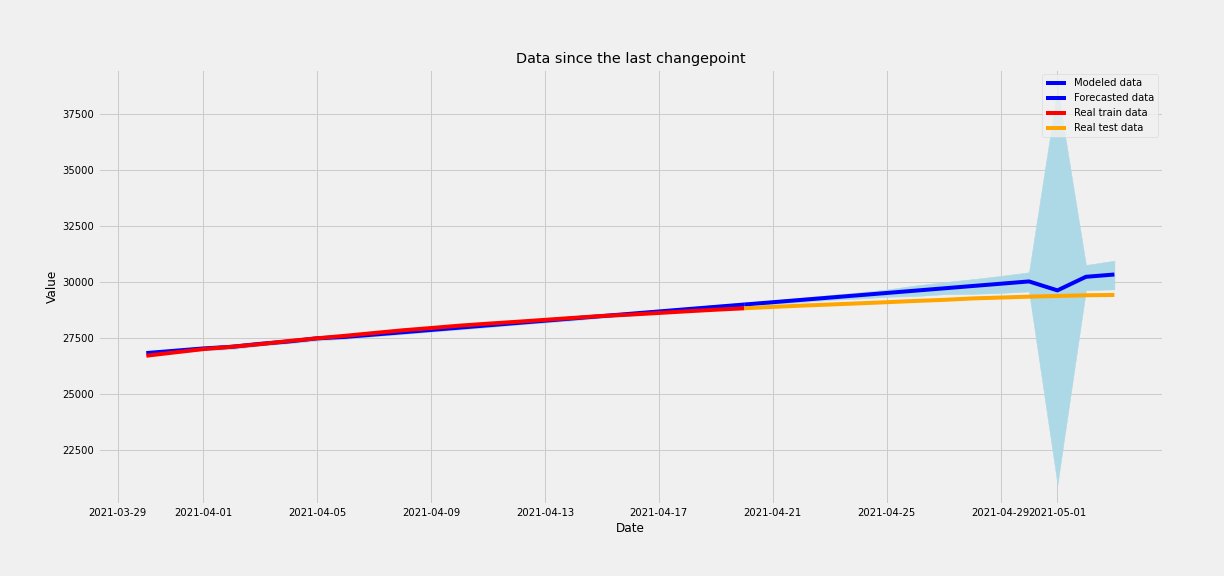
\includegraphics[width=1\textwidth, height=0.28\textwidth]{figures/chapter_04/forecast_example/forecast_dead_fc.png}\label{fig:dead_forecast_last}} \\
\subfloat[d][Number of active cases time series forecast]{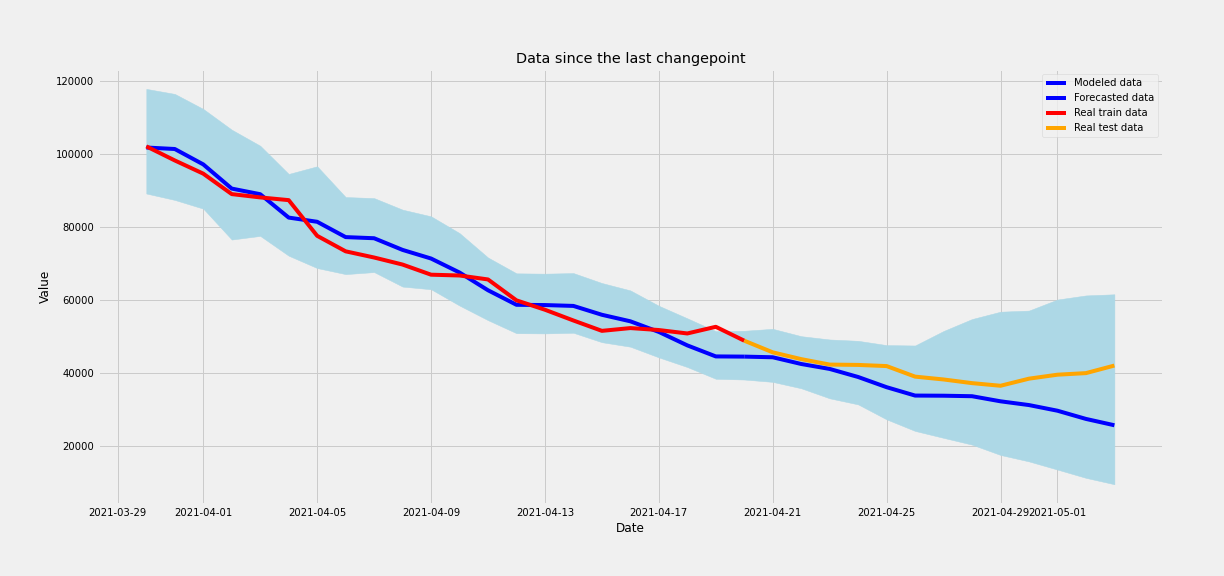
\includegraphics[width=1\textwidth, height=0.28\textwidth]{figures/chapter_04/forecast_example/forecast_active_fc.png}\label{fig:active_forecast_last}} \\
\caption{The selected time series forecasts (since the last detected changepoint May 30, 2021).}
\label{fig:forecast_last}
\end{figure}

In case of the number of active cases time series, we also applied an inverse transformation to compare the forecast with the original data.

According to the graph above, the confidence intervals become dramatically wide after the first forested week. In case of the number of people dead, there is no enough data to include the influence of the Labor day (May 1, 2021), which follows extremely wide confidence intervals. This leads to the fact that only the first several forecasted days may be useful in practice.

In addition to the above visualizations, Table \ref{tab:forecast_results_1} contains information about forecast errors (MAPE). 

\begin{table}[!ht]
\centering
\begin{tabular}{|l|l|}
\hline
Time series                                                                     & Forecast MAPE (\%)\\ \hline
\begin{tabular}[c]{@{}l@{}}Cumulative number \\ of people infected\end{tabular} &  0.818 \\ \hline
\begin{tabular}[c]{@{}l@{}}Cumulative number\\ of people cured\end{tabular}     &     2.143         \\ \hline
\begin{tabular}[c]{@{}l@{}}Cumulative number\\ of people dead\end{tabular}      &      1.597         \\ \hline
\begin{tabular}[c]{@{}l@{}}Number of active\\ cases\end{tabular}                &      14.37         \\ \hline
\end{tabular}%
\caption{Results of the original time series forecast.}
\label{tab:forecast_results_1}
\end{table}

\hypertarget{ss333}{\subsection{Changepoints}}

\subsubsection{Automatically detected changepoints}

While models fitting during the previous subsection, we have obtained a list with the changepoints. It is important to say that the changepoint lists were almost identical for all 4 time series. It is possible, because: all 25 potential changepoints are normally distributed within the first 95\% of the time series (approx. twice a month). 

\begin{table}[!htb]
\centering
\begin{tabular}{|l|l|l|l|l|l||l|l|l|l|l|l|}
\hline
\multicolumn{2}{|l|}{Changepoint}& \multicolumn{4}{l||}{Time series} &\multicolumn{2}{l|}{Changepoint}& \multicolumn{4}{l|}{Time series} \\ \hline
№& Date & I     & C   & D   & A& № & Date & I     & C   & D   & A\\ \hline
1  & 2020-04-06 &    +    &    +    &   +     & + & 14 & 2020-10-17 &    +    &    +    &   +     & +      \\ \hline 
2  & 2020-04-21 &    +    &    +    &   +     & +  & 15 & 2020-11-01 &    +    &    +    &   +     & +      \\ \hline
3  & 2020-05-06 &    +    &    +    &   -     & +  & 16 & 2020-11-16 &    +    &    +    &   +     & +      \\ \hline
4  & 2020-05-21 &    +    &    -    &   +     & +  & 17 & 2020-12-01 &    +    &    +    &   +     & +      \\ \hline
5  & 2020-06-05 &    +    &    -    &   -     & +  & 18 & 2020-12-16 &    -    &    +    &   +     & +      \\ \hline
6  & 2020-06-20 &    +    &    -    &   -     & + &19 & 2020-12-30 &    +    &    +    &   +     & +      \\ \hline  
7  & 2020-07-04 &    +    &    +    &   -     & + &  20 & 2021-01-14 &    +    &    +    &   +     & +      \\ \hline
8  & 2020-07-19 &    -    &    -    &   +     & + & 21 & 2021-01-29 &    +    &    +    &   +     & +      \\ \hline 
9  & 2020-08-03 &    +    &    +    &   -     & + & 22 & 2021-02-13 &    +    &    +    &   +     & +      \\ \hline 
10  & 2020-08-18 &    +   &    -    &   -     & +  & 23 & 2021-02-28 &    +    &    -    &   +     & -      \\ \hline
11 & 2020-09-02 &    +    &    +    &   +     & + & 24 & 2021-03-15 &    +    &    +    &   +     & +      \\ \hline 
12 & 2020-09-17 &    +    &    +    &   +     & + & 25 & 2021-03-30 &    +    &    +    &   +     & +      \\ \hline 
13 & 2020-10-02 &    +    &    +    &   +     & + & - & - &   -   & - &  -  & - \\ \hline 
\end{tabular}
\caption{Automatically detected changepoints (date format: YYYY-MM-DD) including the information about their usage in different models.}
\label{tab:changepoints}
\end{table}
The model tries to find the best changepoints subset with the lowest sum of growth change rate coefficients. In the selected time series, the growth rate changes frequently. and almost all potential changepoints are included in the final subset.

Table \ref{tab:changepoints} contains information about the potential changepoints and their usage in all fitted models. 

It is visible that the final subsets are similar. However, not all potential changepoints were included in every model. 

In this thesis, we will use this changepoints to measure the influence of fitting the model to the slice of the historical data since some changepoints. Thus, we have fitted multiple models to different slices of each selected time series. In Table \ref{tab:slice_forecast} you can see the best forecast results for each time series.

\begin{table}[!hbt]
\centering
\begin{tabular}{|l|l|l|}
\hline
Time series                                                                     & Slice from & MAPE (\%)\\ \hline
\begin{tabular}[c]{@{}l@{}}Cumulative number \\ of people infected\end{tabular} &   2021-01-12 &   0.339   \\ \hline
\begin{tabular}[c]{@{}l@{}}Cumulative number \\ of people cured\end{tabular}    &    2020-12-30   &   0.291 \\ \hline
\begin{tabular}[c]{@{}l@{}}Cumulative number \\ of people dead\end{tabular}    &       2021-02-13     &  0.435     \\ \hline
\begin{tabular}[c]{@{}l@{}}Number of active\\ cases\end{tabular}                &     2020-09-17     &  7.993     \\ \hline
\end{tabular}
\caption{Best results obtained from model fit to the slice of original data (from the changepoint).}
\label{tab:slice_forecast}
\end{table}

As expected, the models that are fitted to the data slice, since some of the specified changepoints are more accurate, then the models that are fitted to all historical data. However, according to the following visualizations (Figure \ref{fig:forecast_last_b}), the confidence intervals are increasing even faster then before. 

It is important to admit that  we have disabled the holidays component, because it is not possible to compute their influence on the final forecast.

\begin{figure}[!ht]
\centering
\subfloat[a][Cumulative number of people infected time series forecast (fitted to the data since January 12, 2021)]{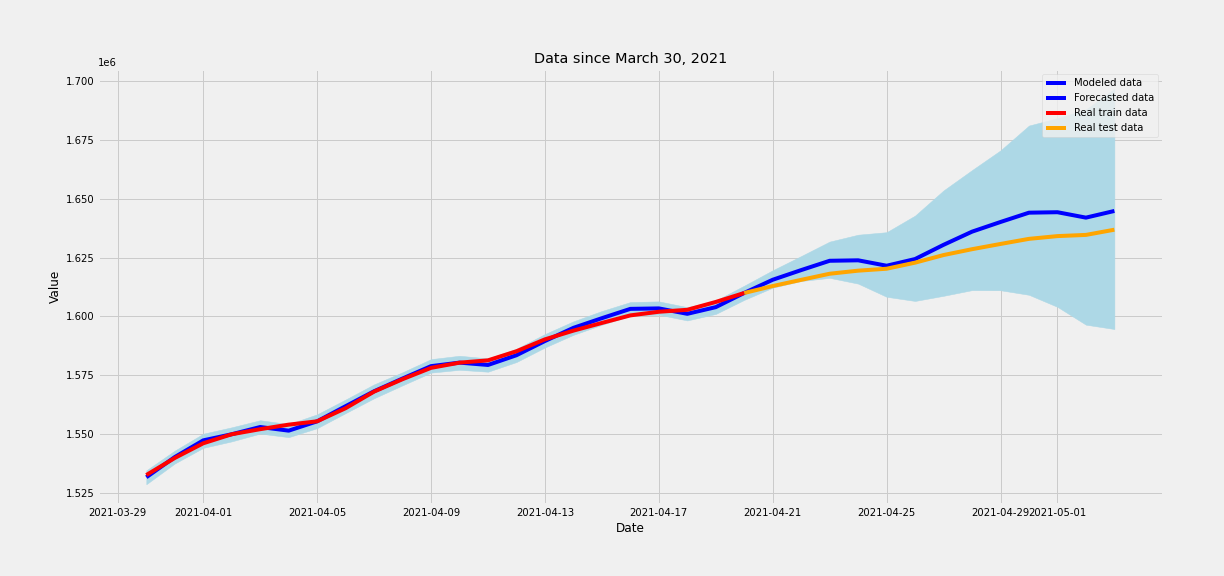
\includegraphics[width=1\textwidth, height=0.26\textwidth]{figures/chapter_04/forecast_example/forecast_infected_b_fc.png}\label{fig:infected_forecast_last_b}} \\
\subfloat[b][Cumulative number of people cured time series forecast (fitted to the data since December 30, 2020)]{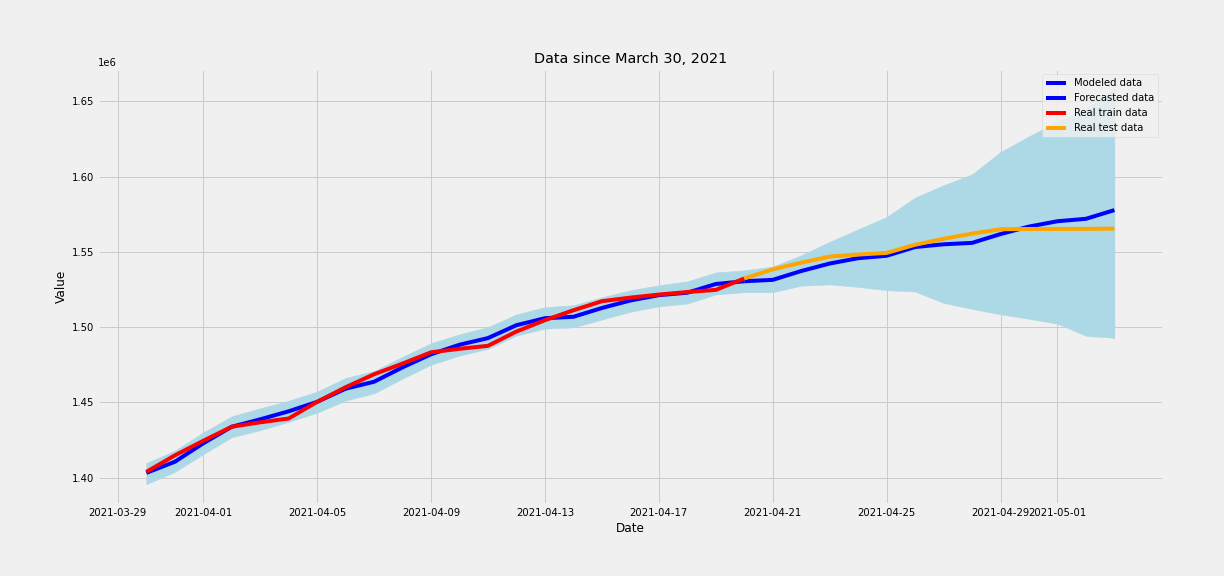
\includegraphics[width=1\textwidth, height=0.26\textwidth]{figures/chapter_04/forecast_example/forecast_cured_b_fc.png}\label{fig:cured_forecast_last_b}} \\
\subfloat[c][Cumulative number of people dead time series forecast (fitted to the data since February 13, 2021)]{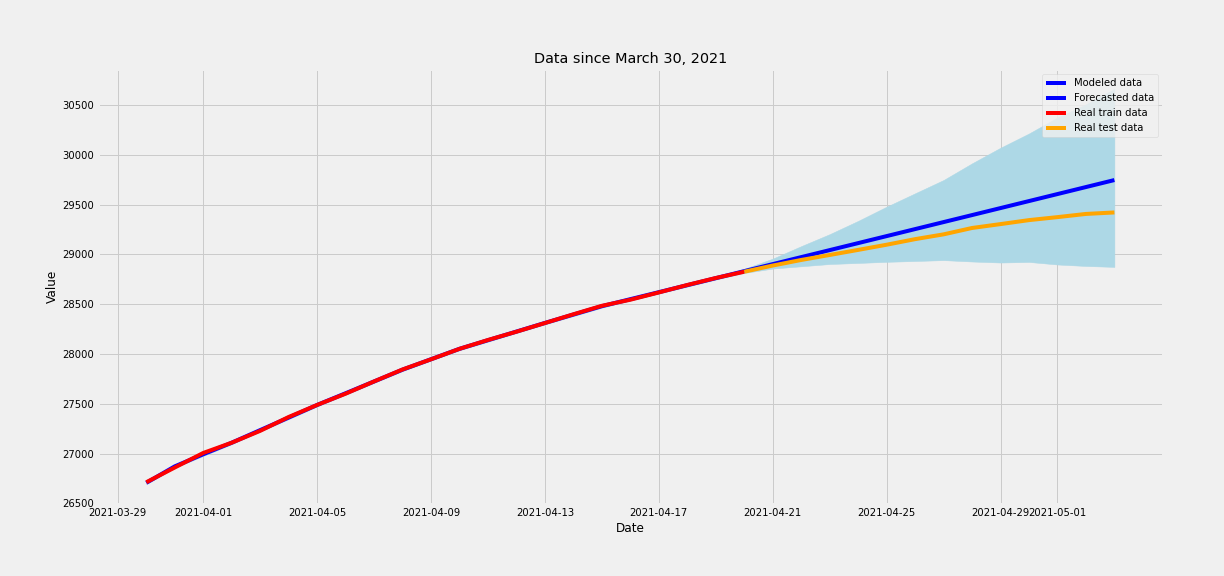
\includegraphics[width=1\textwidth, height=0.26\textwidth]{figures/chapter_04/forecast_example/forecast_dead_b_fc.png}\label{fig:dead_forecast_last_b}} \\
\subfloat[d][Number of active cases time series forecast (fitted to the data since September 17, 2020)]{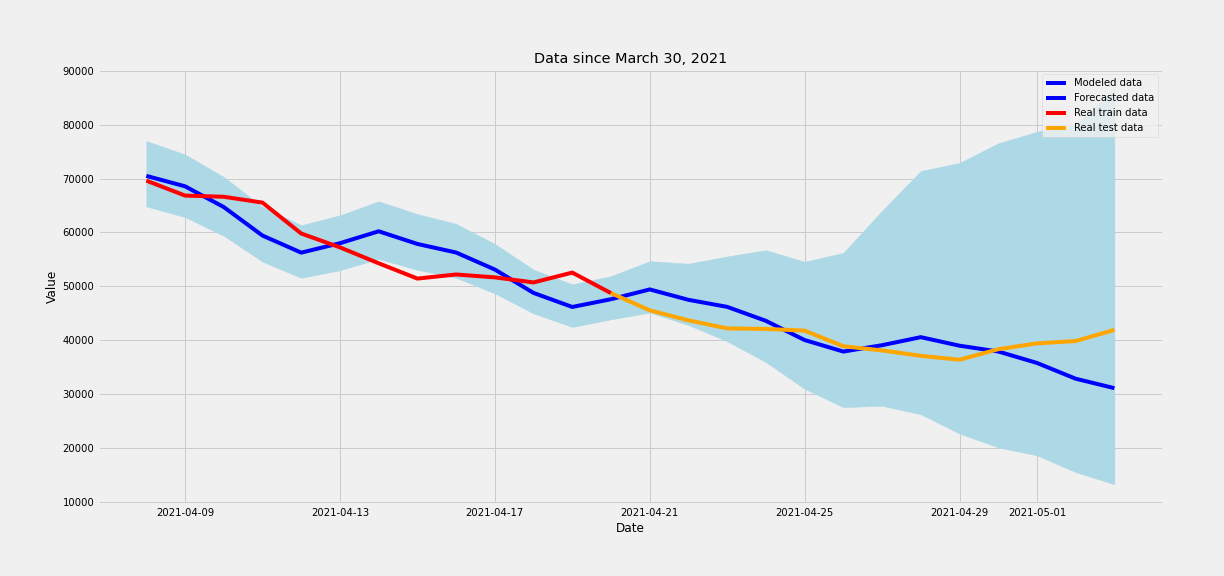
\includegraphics[width=1\textwidth, height=0.26\textwidth]{figures/chapter_04/forecast_example/forecast_active_b_fc.png}\label{fig:active_forecast_last_b}} \\
\caption{The selected time series forecasts (since March 30, 2021) fitted to the slice of data since the specified changepoint.}
\label{fig:forecast_last_b}
\end{figure}
\clearpage

\hypertarget{ss3.3.4}{\subsection{Interesting correlations between changepoints and government restrictions}}

One of the most interesting parts of this work is studying of the correlations between changepoints detected by the Prophet model (and their corresponding trend growth rate changes) and the list of government restrictions during the pandemic.

To perform this analysis, we have prepared the list of government restrictions since March 2, 2020. We have created our own list with 53 different restriction packs and other important events using the covid portal sponsored by the Ministry of the Interior of the Czech Republic \cite{covidportal}.

In this section, we will introduce some important and potentially useful correlations between changes in trend growth rate and some precursory measures before them.

\subsubsection{Correlation: Number of infected explosive growth slowdown}

The following figure shows a slice of the time series that contains measurements between October and January (year 2020). 

\begin{figure}[!ht]
\centering
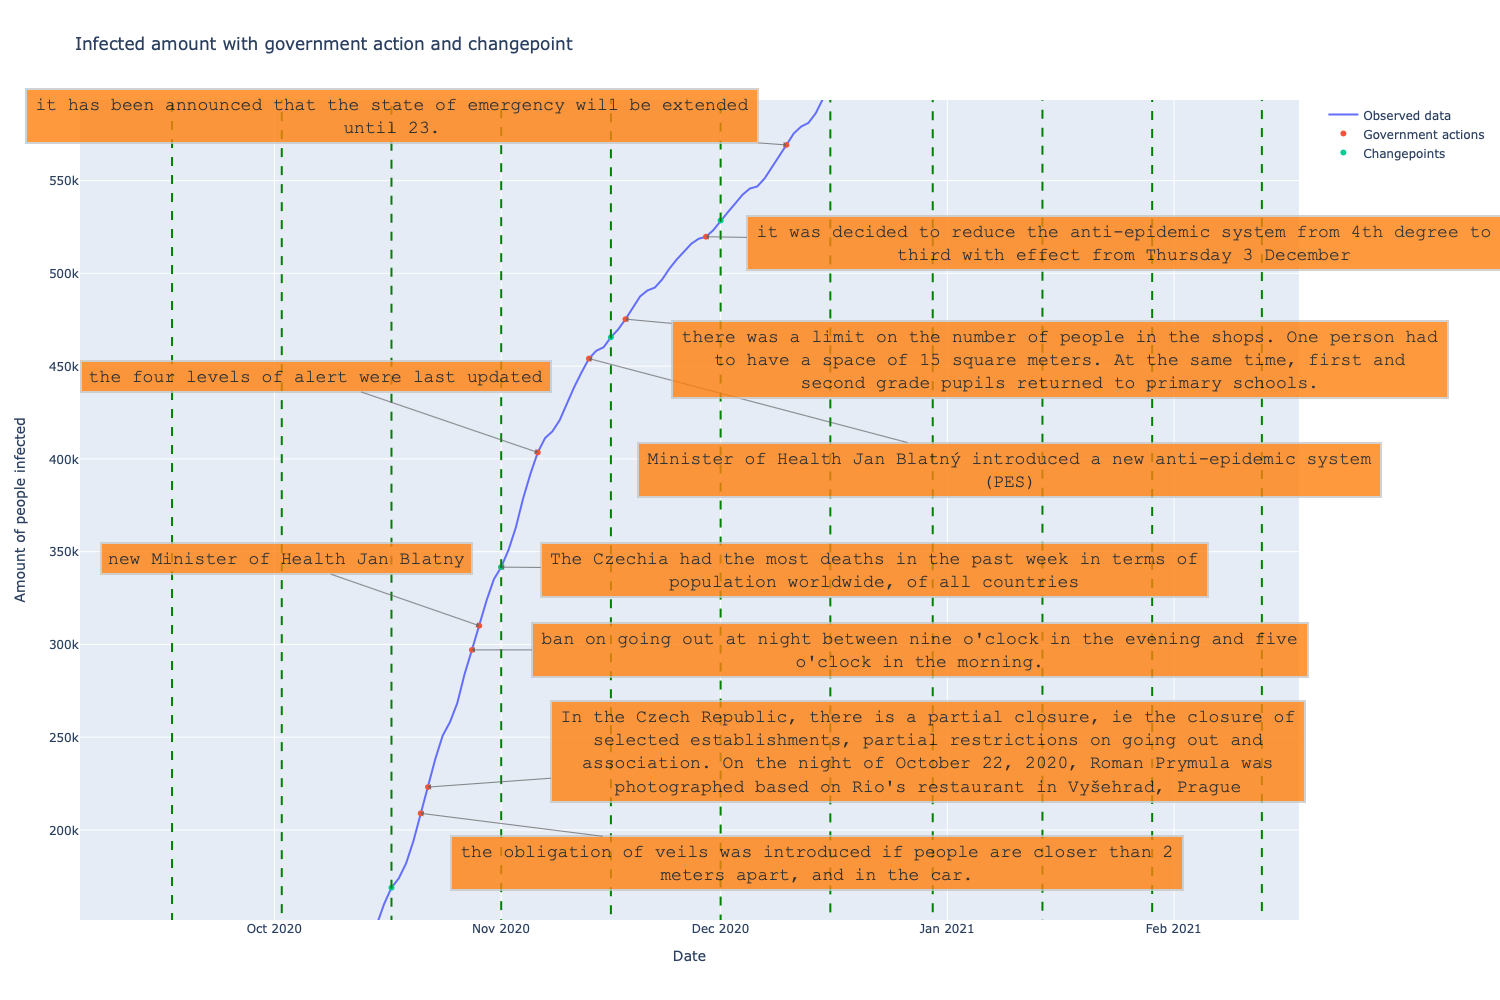
\includegraphics[width=1.0\textwidth, height=0.6\textwidth]{figures/chapter_04/changepoints_vs_government/infecred_expo_to_lin.png}
\caption{Cumulative number of infected growth slowdown October--November 2020.}
\label{fig:corr_inf_e_l}
\end{figure}

During this period, the increase in the number of cases has slowed from a sharply explosive to a calmer (potentially linear) but still rapid growth. The mean number of new cases between neighboring changepoints can be found in Table \ref{tab:new_cases_mean}. It decreased from 11665 to 4209.7 ($-227\%$).

\begin{table}[!htb]
\centering
\begin{tabular}{|l|l|l|}
\hline
Start date & End date & Mean number of active cases \\ \hline
2020-10-17 & 2020-11-01 &   11665.0  \\ \hline
2020-11-01 & 2020-11-16 &   8337.3  \\ \hline
2020-11-16 & 2020-12-01 &   4209.7  \\ \hline
\end{tabular}
\caption{Mean number of new cases daily between October 17, 2020 and December 1, 2020.}
\label{tab:new_cases_mean}
\end{table}

This change may indicate that the government restrictions occurred at a reasonable distance before they are potentially effective. In Figure \ref{fig:corr_inf_e_l} it is possible to see some labels that contain short descriptions of the restrictions between October 15, 2020, and December 15, 2020. \textbf{The most important are}: 
\begin{itemize}
    \item The obligation of face masks if people are closer than meters 2 apart (October 21, 2020).
    \item Partial closure (closure of selected establishments, October 22, 2020).
    \item Ban on going out at night between nine o'clock in the evening and five o'clock in the morning (October 28, 2020).
\end{itemize}

\subsubsection{Correlation: Number of infected explosive growth slowdown 2}

The second interesting slope change is depicted in Figure \ref{fig:corr_inf_e_l_2}. It occurs during the period between February 13, 2021 and May 3, 2021.

According to Table \ref{tab:new_cases_mean_2}, during February and the first half of March, the mean number of people infected daily had increased from 10169 to 11126. However, after March 15, it started to slow down to 3256 (on average) new cases daily ($-341\%$). 

\begin{table}[!htb]
\centering
\begin{tabular}{|l|l|l|}
\hline
Start date & End date & Mean number of active cases \\ \hline
2021-02-13 & 2021-02-28 & 10169.4 \\ \hline
2021-02-28 & 2021-03-15 & 11126.5 \\ \hline
2021-03-15 & 2021-03-30 & 8083.3 \\ \hline
2021-03-30 & 2020-05-03 & 3256.9 \\ \hline
\end{tabular}
\caption{Mean number of new cases daily between February 13, 2021 and May 3, 2021.}
\label{tab:new_cases_mean_2}
\end{table}

This slope change may indicate that potentially effective restrictions were in place prior to this period.

\begin{figure}[!htb]
\centering
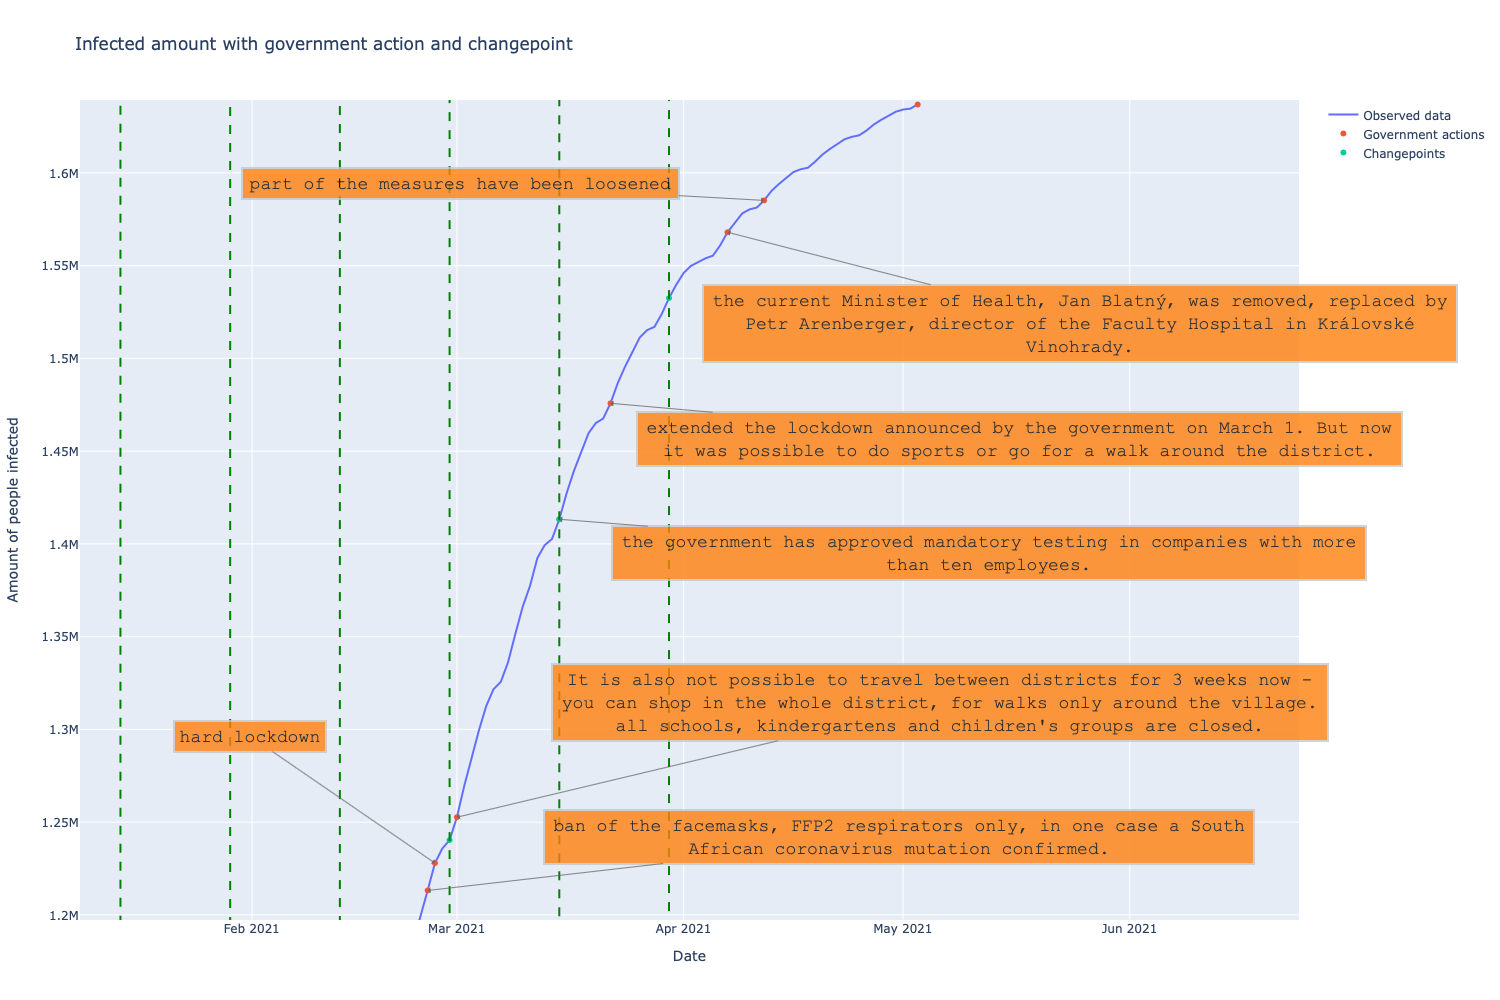
\includegraphics[width=1.0\textwidth, height=0.5\textwidth]{figures/chapter_04/changepoints_vs_government/infected_expo_to_lin_2nd}
\caption{Cumulative number of infected growth slowdown February-May 2021.}
\label{fig:corr_inf_e_l_2}
\end{figure}

We found out that before and during this time interval, the Czech government introduced the following important orders:
\begin{itemize}
    \item Wearing face masks was prohibited, FFP2 respirators only. (February 25, 2021).
    \item Hard lockdown was announced (February 26, 2021).
    \item Travel ban between districts for 3 weeks. All schools, kindergartens, and children's groups were closed. (March 1, 2021).
    \item Mandatory testing in companies with more than ten employees has been approved (March 15, 2021).
\end{itemize}

\subsubsection{Correlation: Number of infected explosive growth slowdown 3}

It is important to mention a growth slowing during the spring of 2020 (Figure \ref{fig:corr_inf_summer}). At this time, the Czech Republic has faced the beginning of the COVID-19 pandemic. According to Table \ref{tab:new_cases_mean_3}, mean number of people infected daily increased from 65.7 to 154.3 ($+234\%$) and then reduced to 66.5 ($-232\%$). 

\begin{table}[!htb]
\centering
\begin{tabular}{|l|l|l|}
\hline
Start date & End date & Mean number of active cases \\ \hline
2020-03-01 & 2020-04-06 & 65.7\\ \hline
2020-04-06 & 2020-04-21 & 154.3\\ \hline
2020-04-21 & 2020-05-06 & 66.5\\ \hline
\end{tabular}
\caption{Mean number of new cases daily between April 6, 2020 and May 6, 2020.}
\label{tab:new_cases_mean_3}
\end{table}

We discovered that before the beginning of the explosive increase of new cases, the government introduced the following important restrictions:
\begin{itemize}
    \item All primary, secondary, higher vocational, and university schools in the Czech Republic were closed until further notice (March 11, 2020).
    \item A state of emergency was declared in the Czech Republic for a period of 30 days (March 12, 2020).
    \item The operation of restaurants and shops was banned (March 14, 2020).
    \item State borders have been closed (with a few exceptions, March 16, 2020). 
\end{itemize}

\begin{figure}[!htb]
\centering
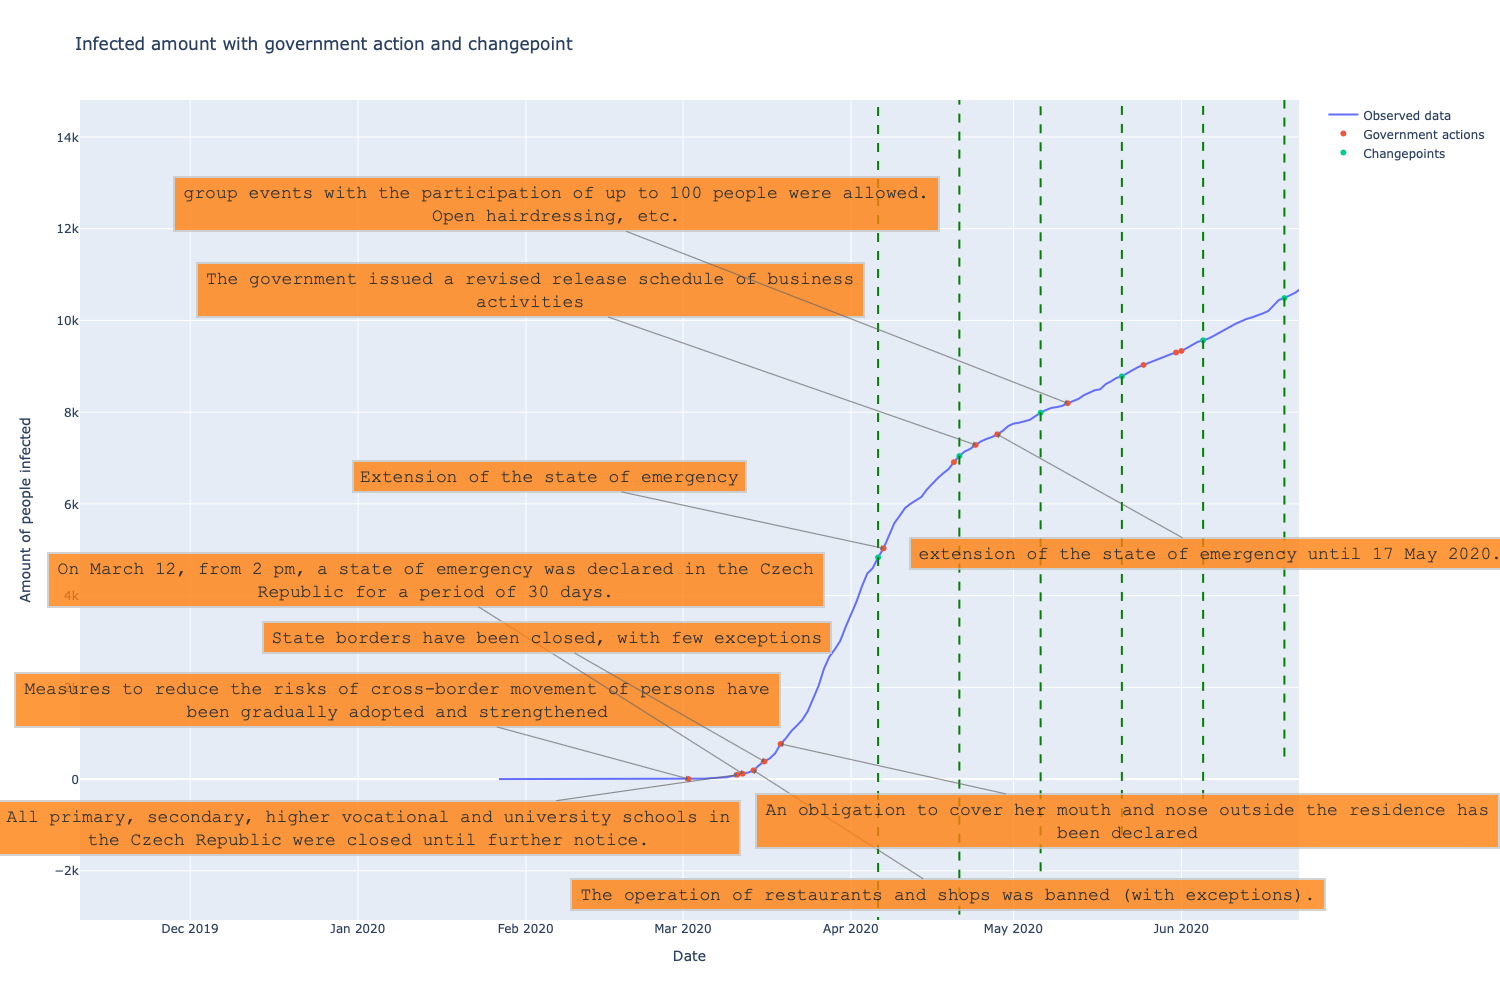
\includegraphics[width=1.0\textwidth, height=0.5\textwidth]{figures/chapter_04/changepoints_vs_government/infected_summer_stop.png}
\caption{Cumulative number of infected growth slowdown April-May 2020.}
\label{fig:corr_inf_summer}
\end{figure}

\subsection{Residual analysis}

Residual analysis is a fundamental step of the model diagnostics process. Thus, we decided to test the models introduced in Subsection \hyperlink{ss332}{3.3.2} and Subsection \hyperlink{ss333}{3.3.3}. 

\begin{figure}[!ht]
\centering
\subfloat[a][Cumulative number of new cases model: Residual analysis.]{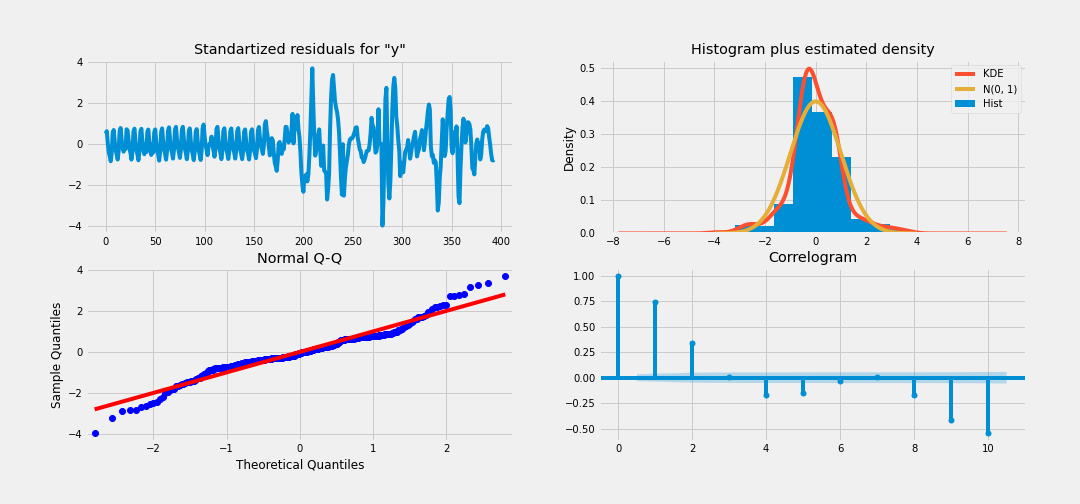
\includegraphics[width=1.0\textwidth, height=0.28\textwidth]{figures/chapter_04/prophet_resid_analysis/resid_prophet_infected.png}\label{fig:resid_infected}} \\
\subfloat[b][Cumulative number of people cured model: Residual analysis.]{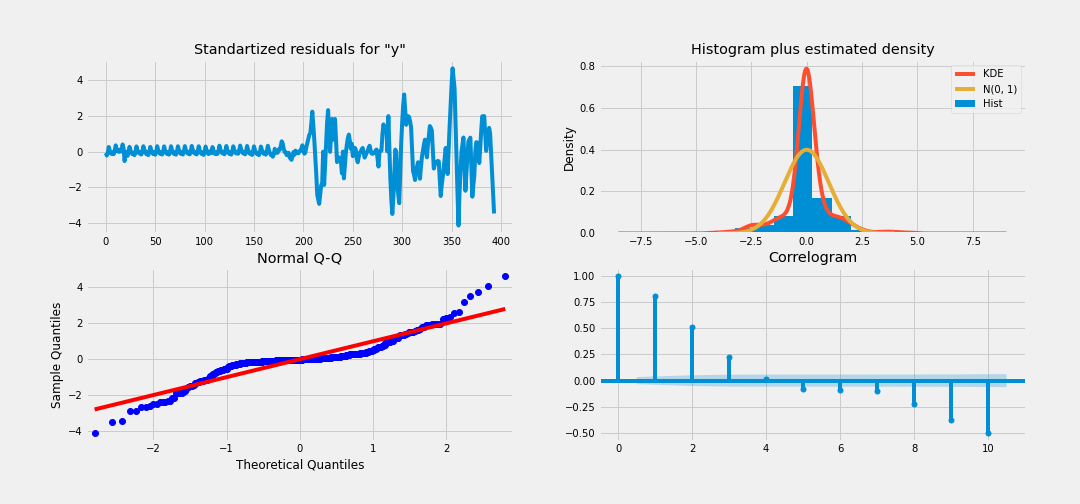
\includegraphics[width=1.0\textwidth, height=0.28\textwidth]{figures/chapter_04/prophet_resid_analysis/resid_prophet_cured.png}\label{fig:resid_cured}} \\
\subfloat[c][Cumulative number of people dead model: Residual analysis.]{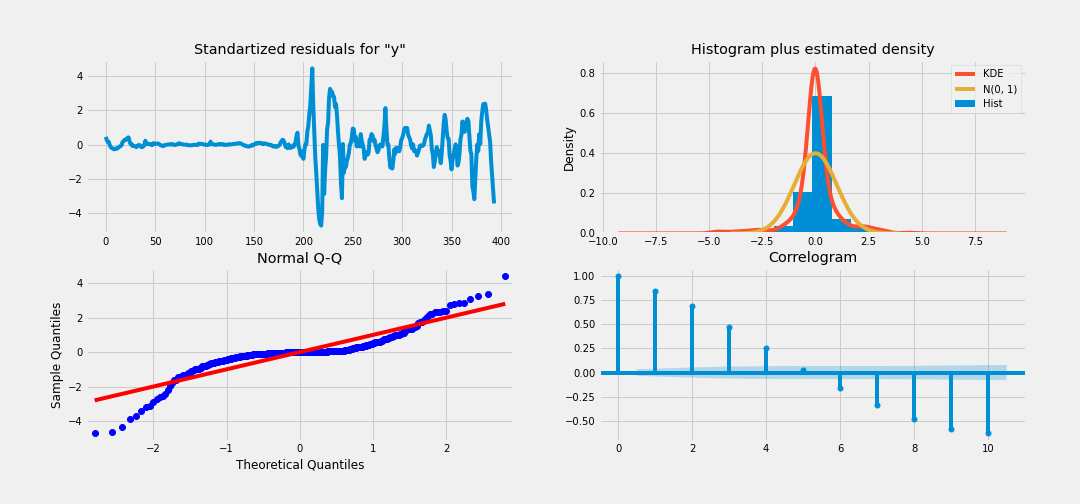
\includegraphics[width=1.0\textwidth, height=0.28\textwidth]{figures/chapter_04/prophet_resid_analysis/resid_prophet_dead.png}\label{fig:resid_dead}} \\
\subfloat[d][Number of active cases model: Residual analysis.]{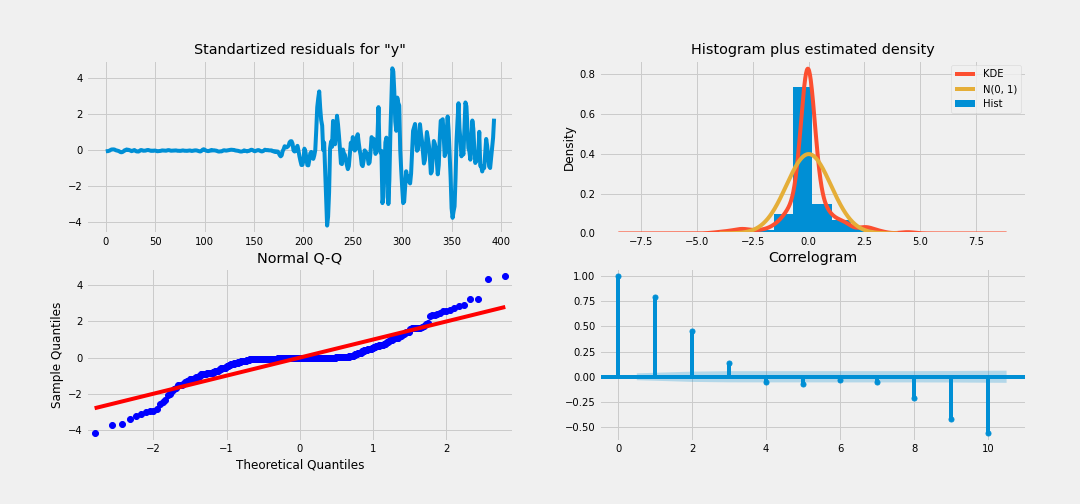
\includegraphics[width=1.0\textwidth, height=0.28\textwidth]{figures/chapter_04/prophet_resid_analysis/resid_prophet_active.png}\label{fig:resid_active}} \\
\caption{Residual analysis for the different Prophet models.}
\label{fig:resid_prophet}
\end{figure}

We consider models fitted to all historical data as more representative (in the context of the whole pandemic) than the models fitted to the data slices since the specific global changepoints and will perform their analysis first.

Analysis pipeline is specified, for example, in Hyndman et al. \cite{Hyndman2018} and contains the statistical testing of the probability that residuals are normally distributed (Jarque-Bera test), testing of the probability of correlation between residuals, and heteroscedasticity testing. Moreover, it implies different visualizations such as Q-Q plot, correlogram, and distribution histogram.

Figure \ref{fig:resid_prophet} demonstrates the different residual diagnostic plots. It is visible that all 4 models have some seasonal correlations between their residuals\footnote{\url{https://github.com/facebook/prophet/issues/1622} --- issue about residual problem in Prophet model. Almost all models have AR(1) relation in residuals. However, seasonal patters may indicate missing or not perfectly estimated seasonality.}. This may indicate that the models do not cover some seasonal relations in the data. Q-Q plots and histograms show that all 4 models do not have a normal distribution of the residuals. Additionally, Table \ref{tab:resid_testing_prophet_all}. contains the results of residual statistical testing\footnote{The Prophet model does not support residual heteroscedasticity testing.} that approve the information received from the visualizations above.

\begin{table}[!hbt]
\centering
\resizebox{\textwidth}{!}{%
\begin{tabular}{|l|l|l|l|}
\hline
Model        & Ljung-Box test                                                & Jarque-Bera test                                              & Heteroscedasticity test \\ \hline
\begin{tabular}[c]{@{}l@{}}Cumulative amount\\ of people infected\end{tabular} &
  \begin{tabular}[c]{@{}l@{}}p-value $\approx$ 0;\\ reject\end{tabular} &
  \begin{tabular}[c]{@{}l@{}}p-value $\approx$ 0;\\ reject\end{tabular} &
  - \\ \hline
\begin{tabular}[c]{@{}l@{}}Cumulative amount \\ of people cured\end{tabular} &
  \begin{tabular}[c]{@{}l@{}}p-value $\approx$ 0;\\ reject\end{tabular} &
  \begin{tabular}[c]{@{}l@{}}p-value $\approx$ 0;\\ reject\end{tabular} &
  - \\ \hline
\begin{tabular}[c]{@{}l@{}}Cumulative amount \\ of people dead\end{tabular} &
  \begin{tabular}[c]{@{}l@{}}p-value $\approx$ 0;\\ reject\end{tabular} &
  \begin{tabular}[c]{@{}l@{}}p-value $\approx$ 0;\\ reject\end{tabular} &
  - \\ \hline
Active cases & \begin{tabular}[c]{@{}l@{}}p-value $\approx$ 0;\\ reject\end{tabular} & \begin{tabular}[c]{@{}l@{}}p-value $\approx$ 0;\\ reject\end{tabular} & -                       \\ \hline
\end{tabular}%
}
\caption{Statistical residual testing of the Prophet models fitted to all historical data.}
\label{tab:resid_testing_prophet_all}
\end{table}

Now we can also perform the statistical residual testing of models fitted to the data slices. Table \ref{tab:resid_testing_prophet_slice} shows that the models fitted to the slices of the data with the information about the number of people cured and dead may have normally distributed residuals. However, we still can not reject that the residuals are correlated.

\begin{table}[!hbt]
\centering
\resizebox{\textwidth}{!}{%
\begin{tabular}{|l|l|l|l|}
\hline
Model        & Ljung-Box test                                                & Jarque-Bera test                                              & Heteroscedasticity test \\ \hline
\begin{tabular}[c]{@{}l@{}}Cumulative amount\\ of people infected\end{tabular} &
  \begin{tabular}[c]{@{}l@{}}p-value $\approx$ 0;\\ reject\end{tabular} &
  \begin{tabular}[c]{@{}l@{}}p-value $\approx$ 0;\\ reject\end{tabular} &
  - \\ \hline
\begin{tabular}[c]{@{}l@{}}Cumulative amount \\ of people cured\end{tabular} &
  \begin{tabular}[c]{@{}l@{}}p-value $\approx$ 0;\\ reject\end{tabular} &
  \begin{tabular}[c]{@{}l@{}}p-value = 0.98;\\ can not reject\end{tabular} &
  - \\ \hline
\begin{tabular}[c]{@{}l@{}}Cumulative amount \\ of people dead\end{tabular} &
  \begin{tabular}[c]{@{}l@{}}p-value $\approx$ 0.0001;\\ reject\end{tabular} &
  \begin{tabular}[c]{@{}l@{}}p-value = 0.21;\\ can not reject\end{tabular} &
  - \\ \hline
Active cases & \begin{tabular}[c]{@{}l@{}}p-value $\approx$ 0;\\ reject\end{tabular} & \begin{tabular}[c]{@{}l@{}}p-value $\approx$ 0;\\ reject\end{tabular} & -                       \\ \hline
\end{tabular}%
}
\caption{Statistical residual testing of the Prophet models fitted to the slices of historical data.}
\label{tab:resid_testing_prophet_slice}
\end{table}

\begin{figure}[!ht]
\centering
\subfloat[a][Cumulative number of new cases model: Residual analysis.]{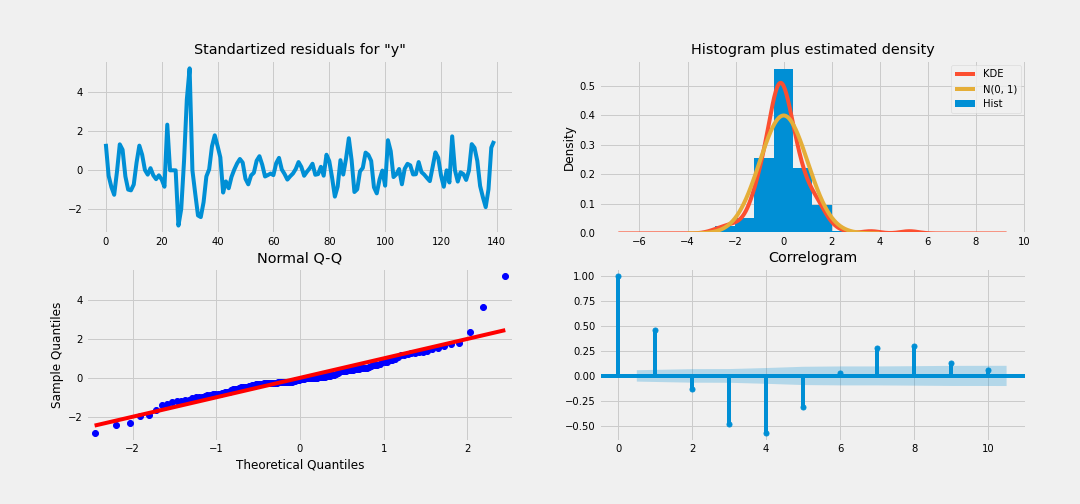
\includegraphics[width=1.0\textwidth, height=0.28\textwidth]{figures/chapter_04/prophet_resid_analysis/resid_prophet_infected_cp.png}\label{fig:resid_infected_slice}} \\
\subfloat[b][Cumulative number of people cured model: Residual analysis.]{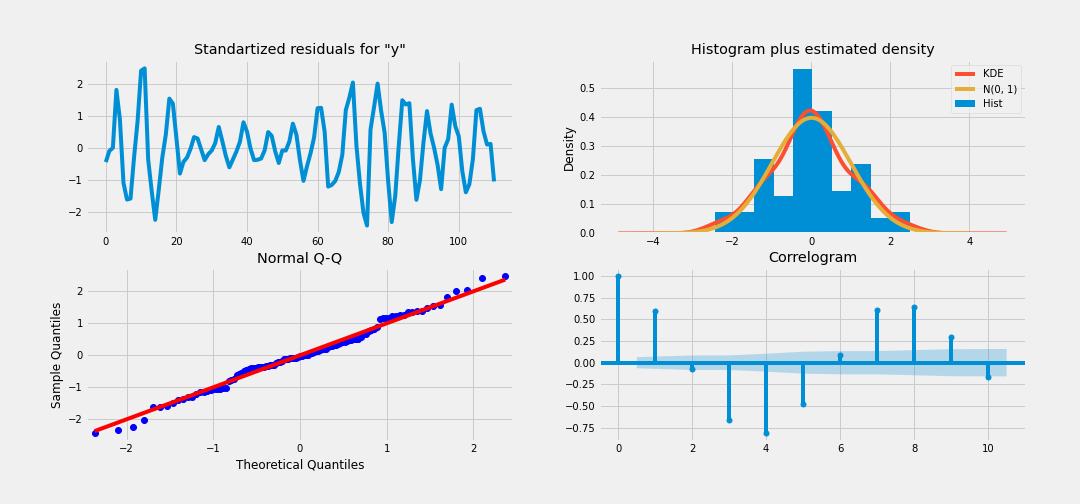
\includegraphics[width=1.0\textwidth, height=0.28\textwidth]{figures/chapter_04/prophet_resid_analysis/resid_prophet_cured_cp.png}\label{fig:resid_cured_slice}} \\
\subfloat[c][Cumulative number of people dead model: Residual analysis.]{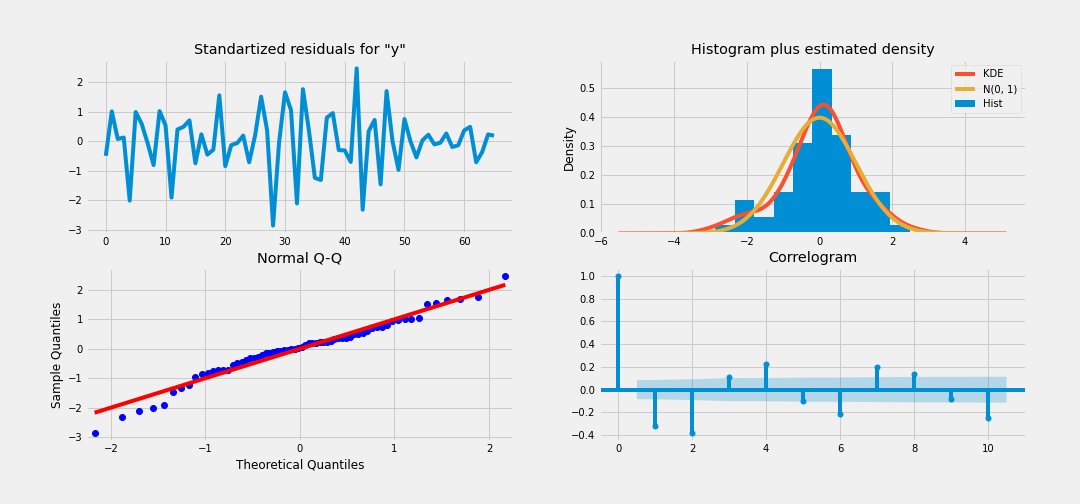
\includegraphics[width=1.0\textwidth, height=0.28\textwidth]{figures/chapter_04/prophet_resid_analysis/resid_prophet_dead_cp.png}\label{fig:resid_dead_slice}} \\
\subfloat[d][Number of active cases model: Residual analysis.]{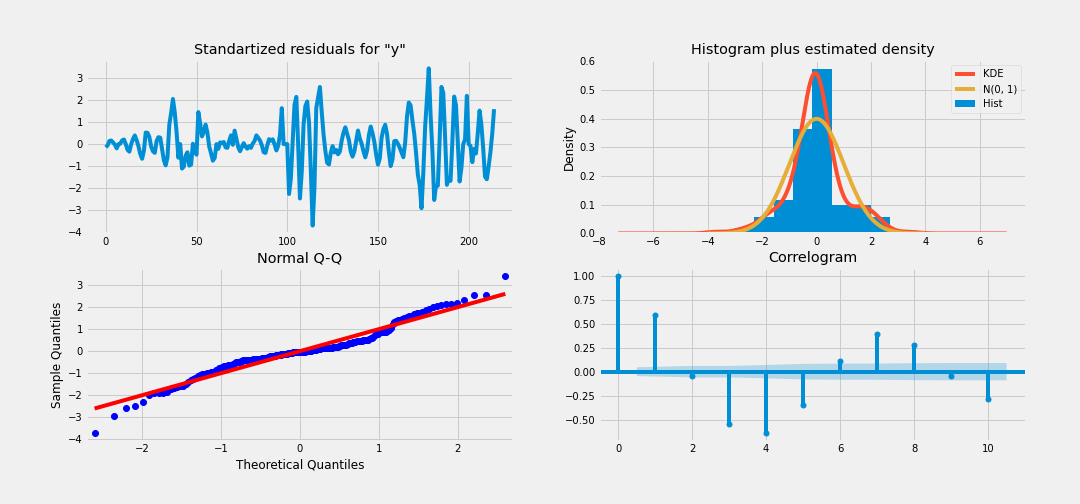
\includegraphics[width=1.0\textwidth, height=0.28\textwidth]{figures/chapter_04/prophet_resid_analysis/resid_prophet_active_cp.png}\label{fig:resid_active_slice}} \\
\caption{Residual analysis for the different Prophet models fitted to the slices of the historical data.}
\label{fig:resid_prophet_slices}
\end{figure}

In Figure \ref{fig:resid_prophet_slices} we can also see that in all models (except for the one that describes the number of deaths) some uncovered seasonal relations occur. The Q-Q plots and histogram indicates that all 4 models now have their residuals distributed more normally. This follows that fitting the model to the slice of the historical data reduces the number of uncovered processes that may influence this data.

% \subsection{Summary}

% // TODO //

\hypertarget{s3.4}{\section{SARIMA modeling}}

In this section, we perform modeling of the selected time series using SARIMA model implemented in Python library named \textit{statsmodels} \cite{seabold2010statsmodels}. It has all important functionalities for model fitting, forecast, and residual analysis.

\subsection{SARIMA model order estimation}

In Section \hypertarget{s3.2}{3.2} we have already estimated the order of the (S)ARIMA models which can be used for modeling the selected time series:
\begin{itemize}
    \item Cumulative number of people infected --- SARIMA(1, 1, 0)$\times$(1, 1, 0$)_7$.
    \item Cumulative number of people cured --- SARIMA(1, 1, 0)$\times$(1, 1, 0$)_7$.
    \item Cumulative number of people dead --- ARIMA(0, 2, 1).
    \item Number of active cases --- SARIMA(1, 1, 0)$\times$(1, 1, 0$)_7$.
\end{itemize}

\subsection{Forecasting using SARIMA}

Similar to the Facebook Prophet forecasts, for SARIMA modeling, we decided to use the 14 days forecast horizon. Moreover, we applied the logarithm transformation to the time series with information about active cases and dropped the first 55 days of measurements (to get rid of measurements with 0 value).

In Table \ref{tab:forecast_results_sarima_1} you can find information about MAPE on train data and on the forecast of new unseen 14 days of data. Models that describe the cumulative sum time series have a forecast MAPE between 0.68 \% and 0.80\%. In difference, the number of active case forecast MAPE is equal to 41.7\%.

\begin{table}[!ht]
\centering
\begin{tabular}{|l|l|l|}
\hline
Time series & Train MAPE & Forecast MAPE (\%)\\ \hline
\begin{tabular}[c]{@{}l@{}}Cumulative number \\ of people infected\end{tabular} &  1.440 &  0.800 \\ \hline
\begin{tabular}[c]{@{}l@{}}Cumulative number\\ of people cured\end{tabular}     &     1.580  &     0.680        \\ \hline
\begin{tabular}[c]{@{}l@{}}Cumulative number\\ of people dead\end{tabular}      &      1.320  &      0.720        \\ \hline
\begin{tabular}[c]{@{}l@{}}Number of active\\ cases\end{tabular}                &     4.710   &      41.760       \\ \hline
\end{tabular}%
\caption{Results of the original time series forecast using SARIMA models.}
\label{tab:forecast_results_sarima_1}
\end{table}

\begin{figure}[!ht]
\centering
\subfloat[a][Cumulative number of people infected time series forecast]{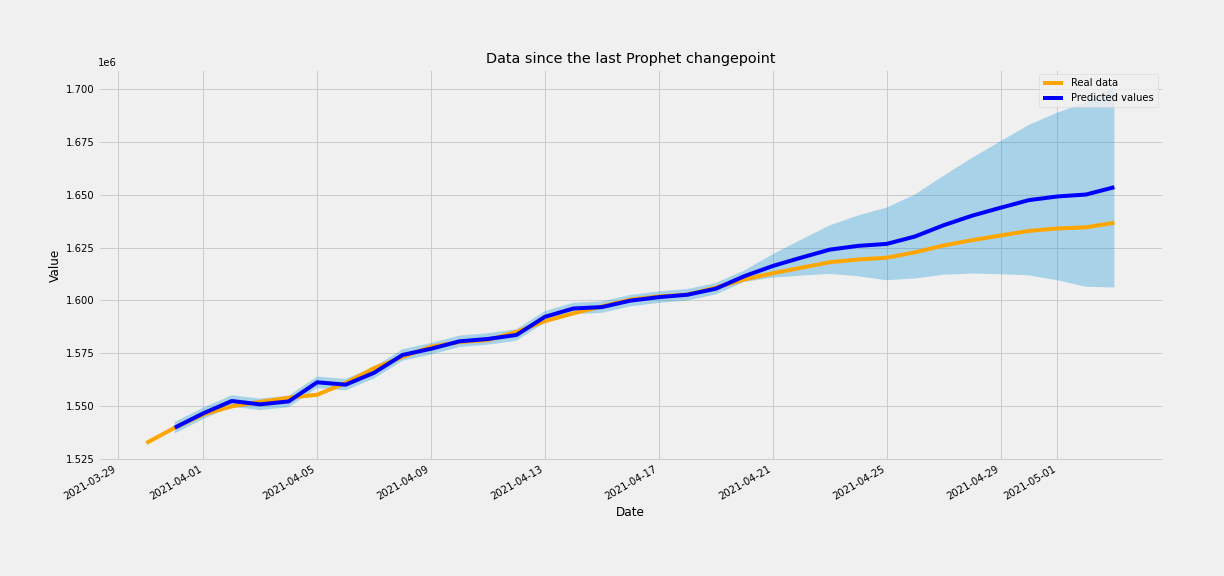
\includegraphics[width=1\textwidth, height=0.28\textwidth]{figures/chapter_04/sarima_forecast/sarima_forecast_infected.png}\label{fig:sarima_infected_forecast}} \\
\subfloat[b][Cumulative number of people cured time series forecast]{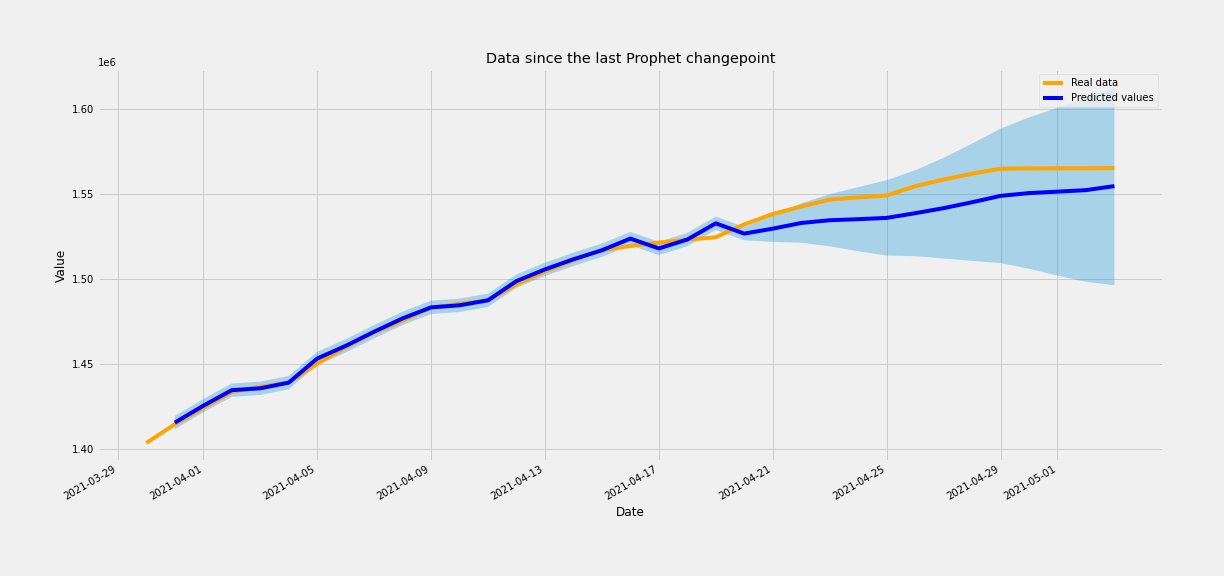
\includegraphics[width=1\textwidth, height=0.28\textwidth]{figures/chapter_04/sarima_forecast/sarima_forecast_cured.png}\label{fig:sarima_cured_forecast}} \\
\subfloat[c][Cumulative number of people dead time series forecast]{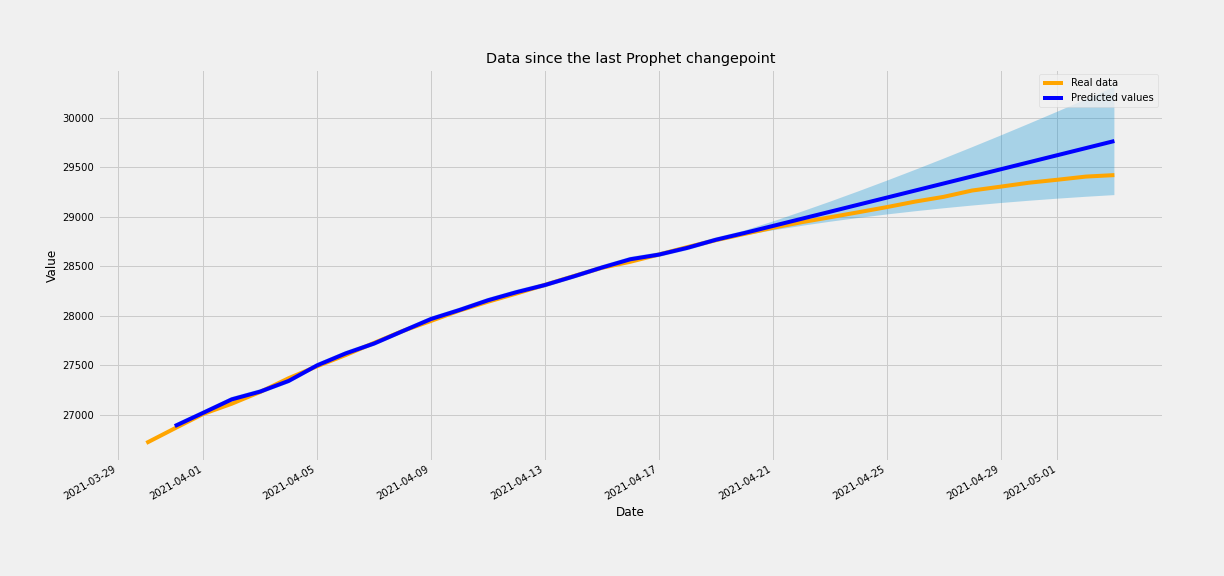
\includegraphics[width=1\textwidth, height=0.28\textwidth]{figures/chapter_04/sarima_forecast/sarima_forecast_dead.png}\label{fig:sarima_dead_forecast}} \\
\subfloat[d][Number of active cases time series forecast]{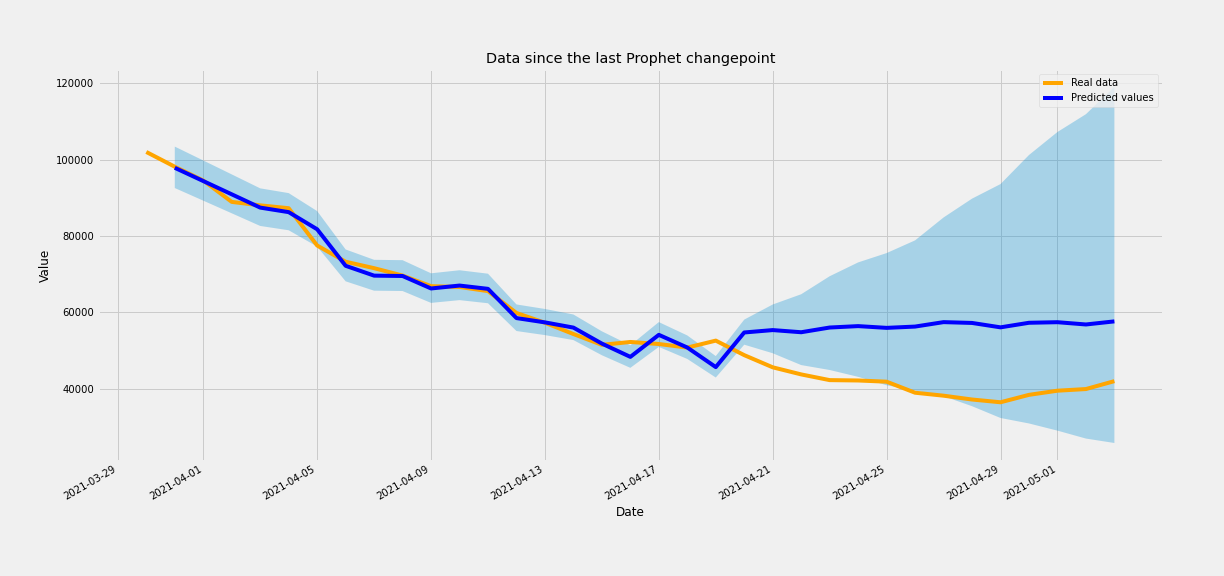
\includegraphics[width=1\textwidth, height=0.28\textwidth]{figures/chapter_04/sarima_forecast/sarima_forecast_active.png}\label{fig:sarima_active_forecast}} \\
\caption{The selected time series forecasts using SARIMA model.}
\label{fig:forecast_sarima}
\end{figure}

Figure \ref{fig:forecast_sarima} contains visualizations of the forecasts made. It covers the period since the last changepoint detected by Prophet (March 30, 2021). It is visible that the forecasts are relatively successful. However, the forecasted number of active cases differs distinctly from the real data. Confidence intervals become extremely wide after the first few days of each forecast.

\subsection{Changepoints usage influence on SARIMA model}

In the Prophet modeling section, we discovered that fitting the model to a slice of the historical data may improve the forecast results. This is possible because the selected COVID-19 time series change their development over time. In this subsection, we decided to study the influence of fitting the SARIMA model to the slices of data on the final forecast of the unseen data.

We fitted various models to the slices of the data since every changepoint detected in Section \hyperlink{ss333}{3.3.3}. Table \ref{tab:sarima_results_cp} contains information about the accuracy of the best forecasts obtained in this way for each time series.

\begin{table}[!ht]
\centering
\begin{tabular}{|l|l|l|l|}
\hline
Time series                                                                    & From date & Train MAPE (\%) & Test MAPE (\%) \\ \hline
\begin{tabular}[c]{@{}l@{}}Cumulative number\\ of people infected\end{tabular} &     2020-10-02      &     1.740       &       0.520    \\ \hline
\begin{tabular}[c]{@{}l@{}}Cumulative number \\ of people cured\end{tabular}   &     2020-12-30      &      9.590      &      3.780     \\ \hline
\begin{tabular}[c]{@{}l@{}}Cumulative number\\ of people dead\end{tabular}     &     2020-10-02     &     2.020       &     0.720     \\ \hline
\begin{tabular}[c]{@{}l@{}}Number of active \\ cases\end{tabular}              &     2021-03-15      &      3.620      &      8.950     \\ \hline
\end{tabular}
\caption{Best results of the time series forecast using SARIMA models fitted to the slices of data.}
\label{tab:sarima_results_cp}
\end{table}

According to these measurements, the prediction error of the number of new and active cases reduced from 0.8\% to 0.52\% and from 41.7\% to 8.95\%. However, the cumulative number of people dead forecast error did not change at all, and the cumulative number of people cured forecast error increased from 0.68\% to 3.78\%. 

Figure \ref{fig:forecast_sarima_cp} contains the corresponding forecast visualizations. On average, the confidence intervals became thinner (which indicates a reduction of the forecast uncertainty). Additionally, visualization (Figure \ref{fig:sarima_active_forecast_cp}) of the active case forecast demonstrates significant improvements. 

The results obtained during this experiment are mixed. Thus, we need to analyze the forecast residuals of all fitted models to conclude.


\begin{figure}[!ht]
\centering
\subfloat[a][Cumulative number of people infected time series forecast (data since October 2, 2020)]{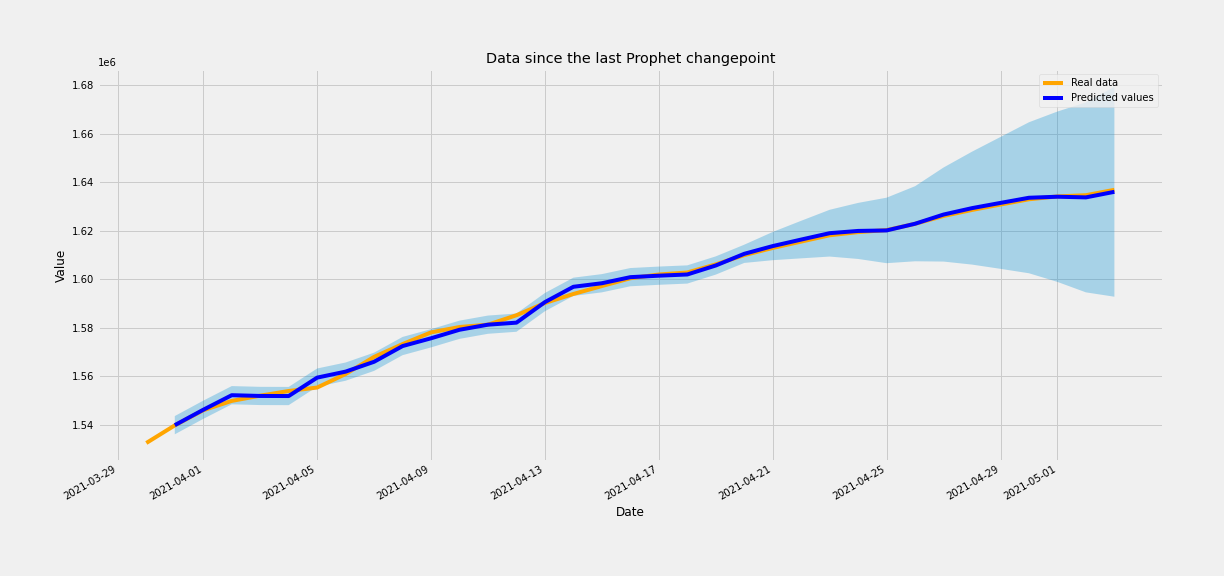
\includegraphics[width=1\textwidth, height=0.25\textwidth]{figures/chapter_04/sarima_forecast/sarima_forecast_infected_cp.png}\label{fig:sarima_infected_forecast_cp}} \\
\subfloat[b][Cumulative number of people cured time series forecast (data since December 30, 2020)]{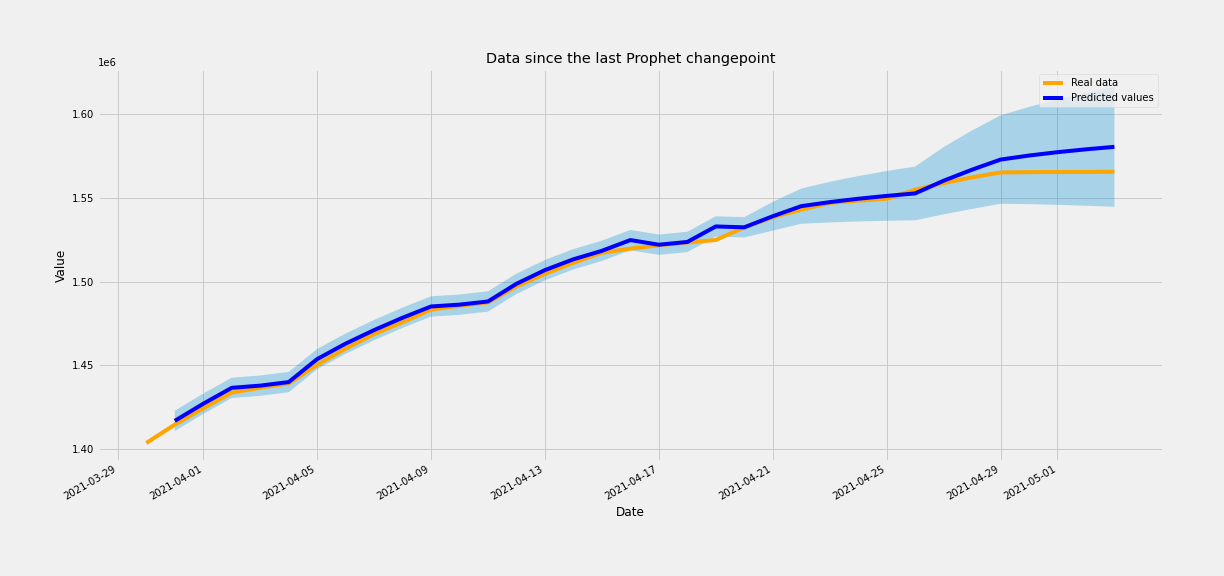
\includegraphics[width=1\textwidth, height=0.25\textwidth]{figures/chapter_04/sarima_forecast/sarima_forecast_cured_cp.png}\label{fig:sarima_cured_forecast_cp}} \\
\subfloat[c][Cumulative number of people dead time series forecast (data since October 2, 2020)]{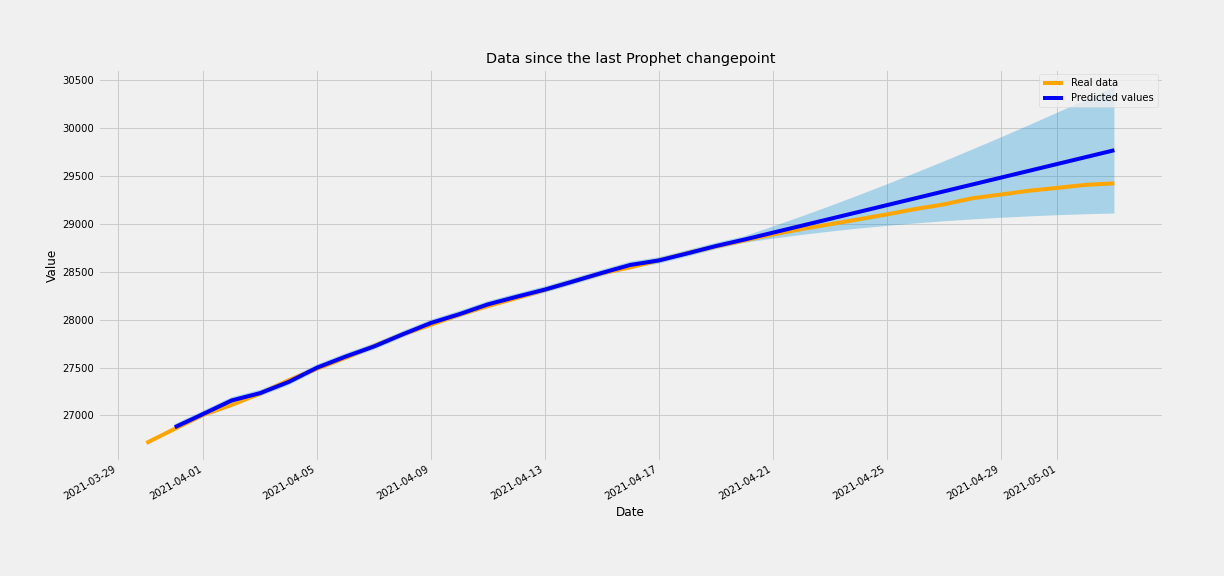
\includegraphics[width=1\textwidth, height=0.25\textwidth]{figures/chapter_04/sarima_forecast/sarima_forecast_dead_cp.png}\label{fig:sarima_dead_forecast_cp}} \\
\subfloat[d][Number of active cases time series forecast (data since March 15, 2021)]{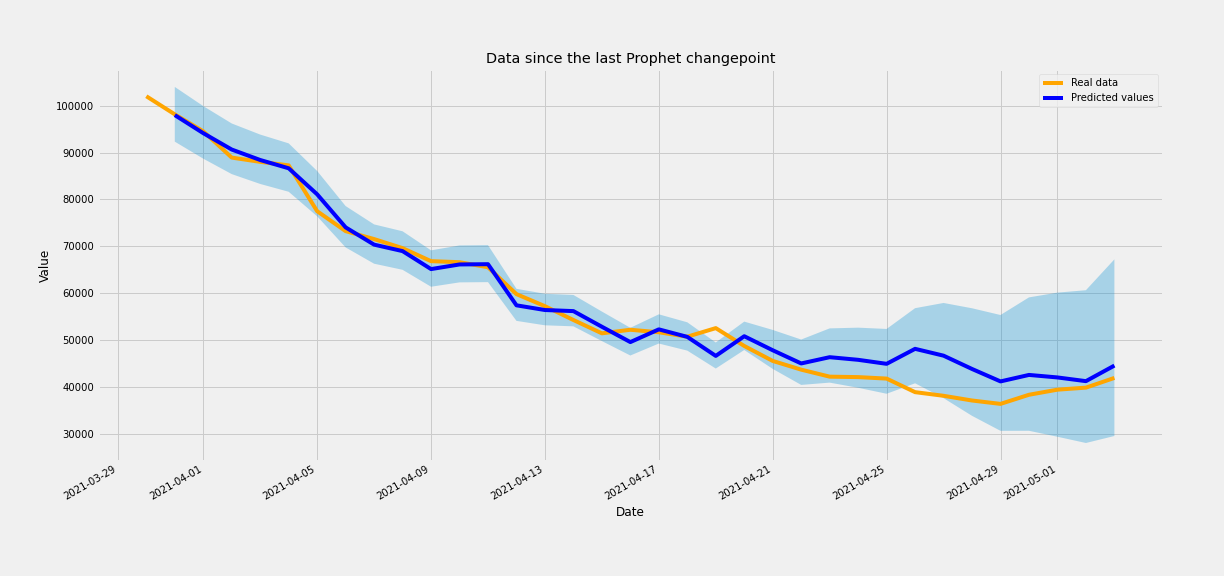
\includegraphics[width=1\textwidth, height=0.25\textwidth]{figures/chapter_04/sarima_forecast/sarima_forecast_active_cp.png}\label{fig:sarima_active_forecast_cp}} \\
\caption{The selected time series forecasts using SARIMA (since March 30, 2021) fitted to the slice of data since the specified changepoint}
\label{fig:forecast_sarima_cp}
\end{figure}

\subsection{Residual Analysis}

After fitting the SARIMA model, statsmodels allows us to perform residual analysis. Similar to the Prophet, we will use residual testing and visualization. 

\begin{figure}[!ht]
\centering
\subfloat[a][Cumulative number of new cases model: Residual analysis.]{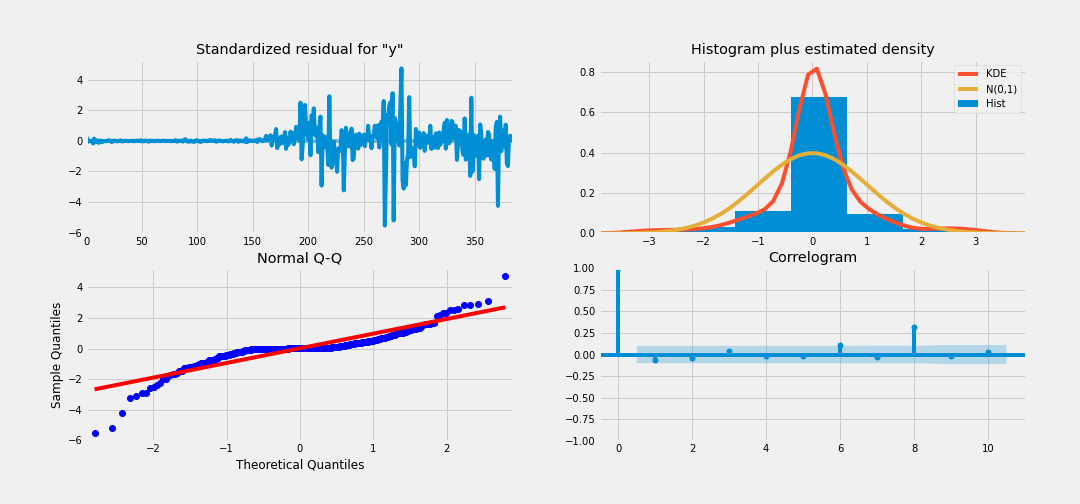
\includegraphics[width=1.0\textwidth, height=0.28\textwidth]{figures/chapter_04/sarima_resid_analysis/residual_sarima_infected.png}\label{fig:resid_infected_s}} \\
\subfloat[b][Cumulative number of people cured model: Residual analysis.]{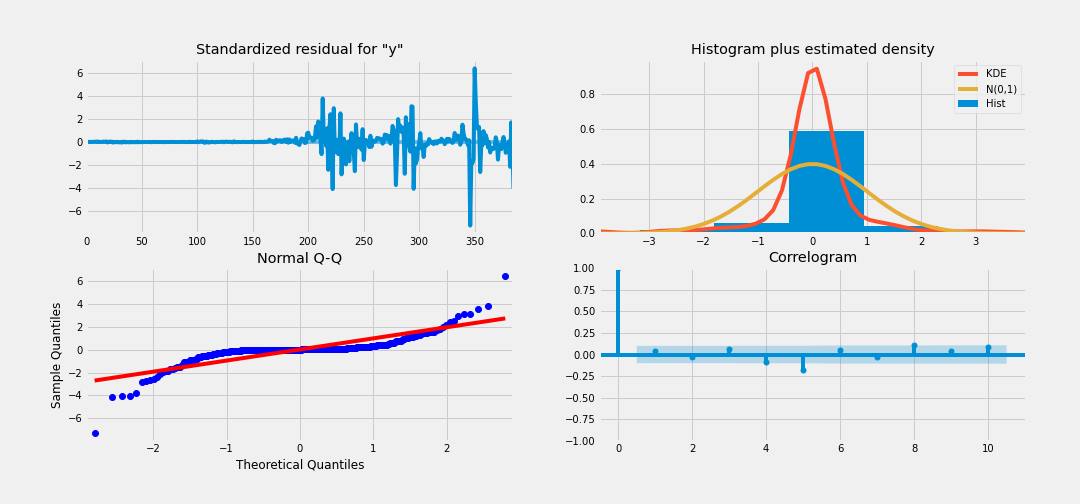
\includegraphics[width=1.0\textwidth, height=0.28\textwidth]{figures/chapter_04/sarima_resid_analysis/residual_sarima_cured.png}\label{fig:resid_cured_s}} \\
\subfloat[c][Cumulative number of people dead: Residual analysis.]{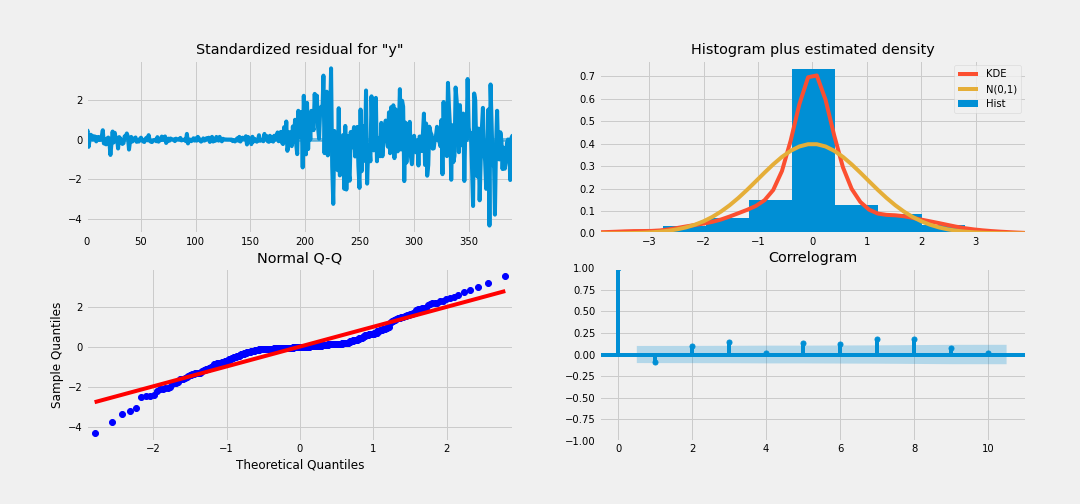
\includegraphics[width=1.0\textwidth, height=0.28\textwidth]{figures/chapter_04/sarima_resid_analysis/residual_sarima_dead.png}\label{fig:resid_dead_s}} \\
\subfloat[d][Cumulative number of active cases: Residual analysis.]{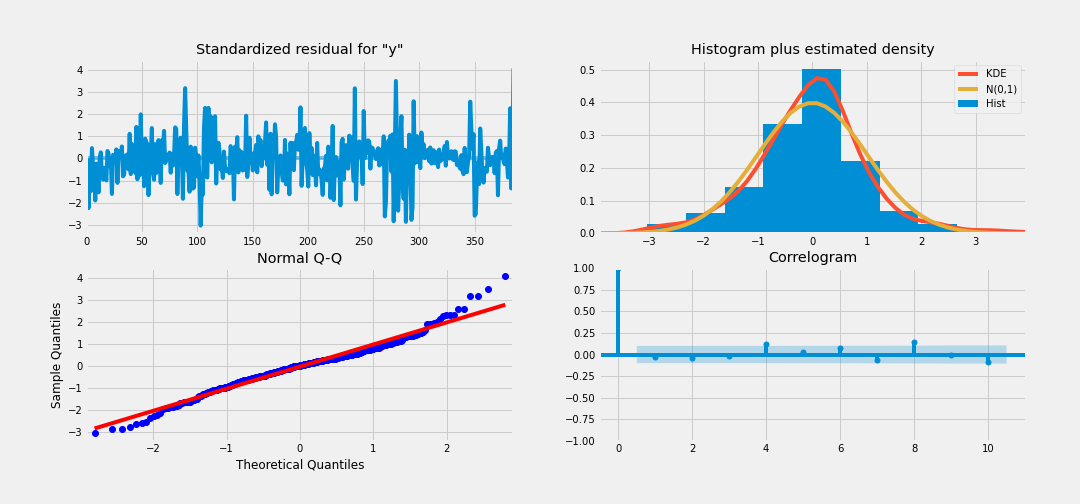
\includegraphics[width=1.0\textwidth, height=0.28\textwidth]{figures/chapter_04/sarima_resid_analysis/residual_sarima_active.png}\label{fig:resid_active_s}}\\
\caption{Residual analysis for the different SARIMA models.}
\label{fig:resid_sarima}
\end{figure}

First, we will analyze the models fitted to all historical data. 

According to Figure \ref{fig:resid_sarima}, number of new cases model has a residual correlation at lag 8, while the other 3 models may have uncorrelated residuals. However, according to the Ljung-Box test (Table \ref{tab:resid_testing_sarima}) we reject the hypothesis that the residuals are not correlated only for the model that describes the cumulative number of people dead time series. 

\begin{table}[!hbt]
\centering
\resizebox{\textwidth}{!}{%
\begin{tabular}{|l|l|l|l|}
\hline
Model        & Ljung-Box test                                                & Jarque-Bera test                                              & Heteroscedasticity test \\ \hline
\begin{tabular}[c]{@{}l@{}}Cumulative amount\\ of people infected\end{tabular} &
  \begin{tabular}[c]{@{}l@{}}p-value = 0.23;\\ can not reject\end{tabular} &
  \begin{tabular}[c]{@{}l@{}}p-value = 0.00;\\ reject\end{tabular} &
  \begin{tabular}[c]{@{}l@{}}p-value = 0.00;\\ reject \end{tabular} \\\hline
\begin{tabular}[c]{@{}l@{}}Cumulative amount \\ of people cured\end{tabular} &
  \begin{tabular}[c]{@{}l@{}}p-value = 0.37;\\ can not reject\end{tabular} &
  \begin{tabular}[c]{@{}l@{}}p-value = 0.00;\\ reject\end{tabular} &
  \begin{tabular}[c]{@{}l@{}}p-value = 0.00;\\ reject \end{tabular}\\ \hline
\begin{tabular}[c]{@{}l@{}}Cumulative amount \\ of people dead\end{tabular} &
  \begin{tabular}[c]{@{}l@{}}p-value = 0.00;\\ reject\end{tabular} &
  \begin{tabular}[c]{@{}l@{}}p-value = 0.00;\\ reject\end{tabular} &
  \begin{tabular}[c]{@{}l@{}}p-value = 0.00;\\ reject \end{tabular}\\ \hline
Active cases & \begin{tabular}[c]{@{}l@{}}p-value = 0.60;\\ can not reject\end{tabular} & \begin{tabular}[c]{@{}l@{}}p-value = 0.00;\\ reject\end{tabular} & \begin{tabular}[c]{@{}l@{}}p-value = 0.36;\\ can not reject      \end{tabular} \\ \hline
\end{tabular}%
}
\caption{Statistical residual testing of the SARIMA models fitted to all historical data.}
\label{tab:resid_testing_sarima}
\end{table}

Q-Q plots and histograms indicated that all 4 model residuals are not normally distributed. Jarque-Bera testing confirms it.  

The heteroscedasticity test indicates that the model that describes the number of active cases time series has residuals that do not change their structure over time (more relevant long-term forecasts). However, this result differs from the others because we applied a logarithm transformation to this time series (which reduces the heteroscedasticity in data). 

Now we can move to the residual analysis of the models fitted to the slices of the data since the specified changepoints.

\begin{table}[!hbt]
\centering
\resizebox{\textwidth}{!}{%
\begin{tabular}{|l|l|l|l|}
\hline
Model        & Ljung-Box test                                                & Jarque-Bera test                                              & Heteroscedasticity test \\ \hline
\begin{tabular}[c]{@{}l@{}}Cumulative amount\\ of people infected\end{tabular} &
  \begin{tabular}[c]{@{}l@{}}p-value = 0.00;\\ reject\end{tabular} &
  \begin{tabular}[c]{@{}l@{}}p-value = 0.00;\\ reject\end{tabular} &
  \begin{tabular}[c]{@{}l@{}}p-value = 0.00;\\ reject\end{tabular}\\ \hline
\begin{tabular}[c]{@{}l@{}}Cumulative amount \\ of people cured\end{tabular} &
  \begin{tabular}[c]{@{}l@{}}p-value = 0.00;\\ reject\end{tabular} &
  \begin{tabular}[c]{@{}l@{}}p-value = 0.00;\\ reject\end{tabular} &
  \begin{tabular}[c]{@{}l@{}}p-value = 0.26;\\ can not reject \end{tabular}\\ \hline
\begin{tabular}[c]{@{}l@{}}Cumulative amount \\ of people dead\end{tabular} &
  \begin{tabular}[c]{@{}l@{}}p-value = 0.23;\\ can not reject\end{tabular} &
  \begin{tabular}[c]{@{}l@{}}p-value = 0.73;\\ can not reject\end{tabular} &
  \begin{tabular}[c]{@{}l@{}}p-value = 0.64;\\ can not reject \end{tabular} \\ \hline
Active cases & \begin{tabular}[c]{@{}l@{}}p-value = 0.97;\\ can not reject\end{tabular} & \begin{tabular}[c]{@{}l@{}}p-value = 0.00;\\ reject\end{tabular} & \begin{tabular}[c]{@{}l@{}}p-value = 0.00; \\reject\end{tabular}\\ \hline
\end{tabular}%
}
\caption{Statistical residual testing of the SARIMA models fitted to slices of the historical data.}
\label{tab:resid_testing_sarima_slice}
\end{table}

According to Figure \ref{fig:resid_sarima_cp}, models that describe the cumulative number of people cured and infected now have correlated residuals. Ljung-Box test results (Table \ref{tab:resid_testing_sarima_slice}) confirm that. Their residuals also are not normally distributed.

\begin{figure}[!ht]
\centering
\subfloat[a][Cumulative number of new cases model: Residual analysis.]{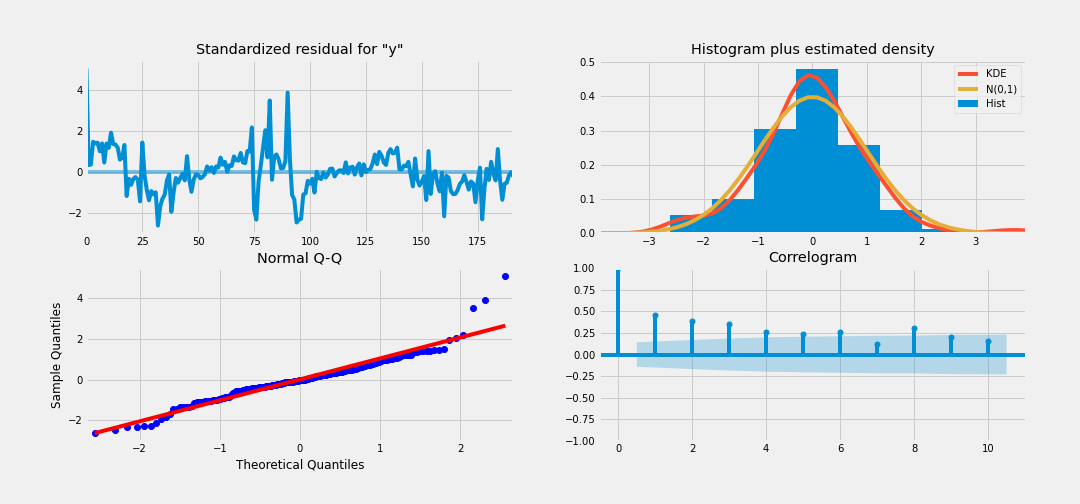
\includegraphics[width=1.0\textwidth, height=0.28\textwidth]{figures/chapter_04/sarima_resid_analysis/residual_sarima_infected_cp.png}\label{fig:resid_infected_s_cp}} \\
\subfloat[b][Cumulative number of people cured model: Residual analysis.]{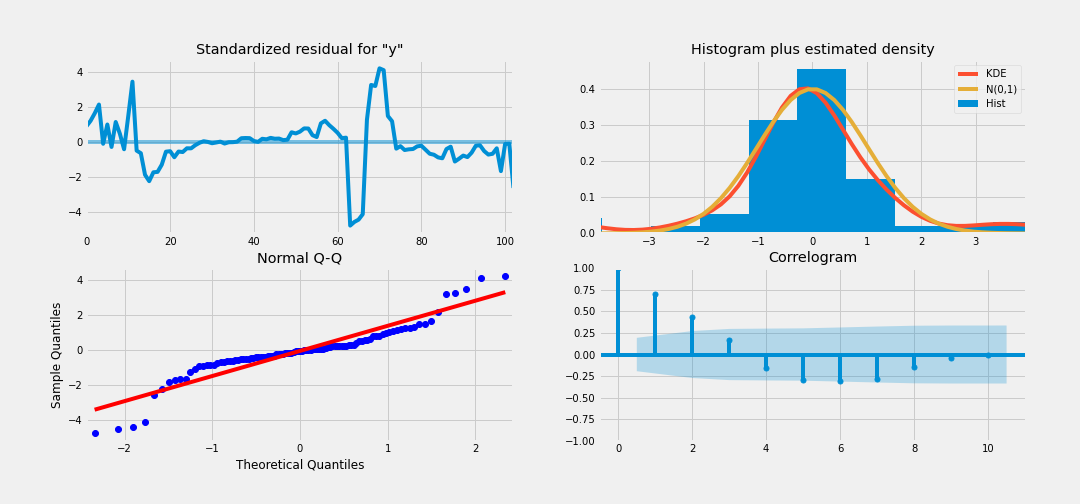
\includegraphics[width=1.0\textwidth, height=0.28\textwidth]{figures/chapter_04/sarima_resid_analysis/residual_sarima_cured_cp.png}\label{fig:resid_cured_s_cp}} \\
\subfloat[c][Cumulative number of people dead: Residual analysis.]{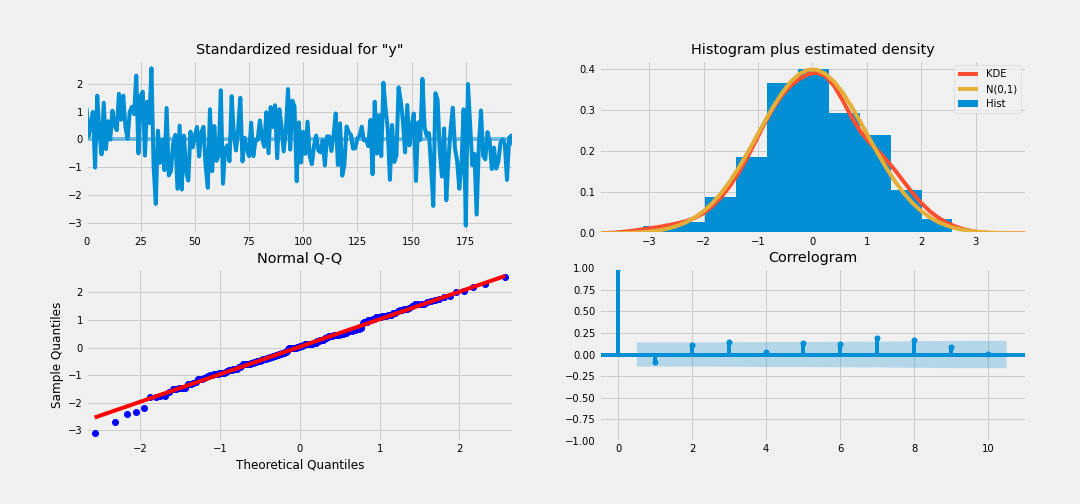
\includegraphics[width=1.0\textwidth, height=0.28\textwidth]{figures/chapter_04/sarima_resid_analysis/residual_sarima_dead_cp.png}\label{fig:resid_dead_s_cp}} \\
\subfloat[d][Number of active cases: Residual analysis.]{\includegraphics[width=1.0\textwidth, height=0.28\textwidth]{figures/chapter_04/sarima_resid_analysis/residual_sarima_active_cp.png}\label{fig:resid_active_s_cp}}\\
\caption{Residual analysis for the different SARIMA models fitted to the slices of data since specified changepoints.}
\label{fig:resid_sarima_cp}
\end{figure}

However, the number of people cured time series has heteroscedastic residuals (which may be helpful for long-term forecasts). 

The number of people dead model has noncorrelated, potentially normally distributed, heteroscedastic residuals and may be potentially used for long-term forecasts.

The number of active cases model also has noncorrelated residuals, but they are not heteroscedastic and not normally distributed.

\section{Results evaluation and discussion}

\subsection{Time series analysis results evaluation}

In Section \hyperlink{s3.2}{3.2} we performed the basic analysis of the selected time series. Using the theory studied during the theoretical research, we have found that:
\begin{itemize}
    \item It is possible to separate different processes and components that influence the evolution of the COVID-19 time series, such as global trend or seasonality (using the ACF and PACF).
    \item It is possible to estimate the order of the SARIMA model that can be used for modeling these time series, using methods that remove global trend and seasonality (differencing).
    \item The selected time series are changing their behavior over time. This fact requires the usage of models that can handle these changes.
\end{itemize}

This information is helpful for future analysis steps and reduces the number of problems that may occur during time series modeling using the Facebook Prophet or SARIMA model.

\subsection{Facebook Prophet modeling results evaluation}

In Section \hyperlink{s3.3}{3.3} we studied the possibility of modeling the COVID-19 time series using the Facebook Prophet model and obtained some interesting results. 

First, we discovered that it is possible to estimate proper hyperparameters using the inbuilt cross-validation technique. Models fitted using these parameters can achieve reasonable results.


Interestingly, the time series that contain the cumulative number of people infected, people cured, and people dead can be modeled without any data transformation. The number of active cases time series requires logarithm or Box-Cox transformation to reduce the measure of structural changes in the data. The forecasts made using the Prophet model fitted to all historical data are relatively accurate: the cumulative sum time series forecast error is within 0.8\% and 2.1\%. However, the number of active case predictions on average have 14\% error.  

Unexpectedly, the Facebook Prophet model residual analysis process has some potential problems (due to an incomplete model component). However, it is possible to detect some changes not covered by our models.

As expected, using the piecewise model allowed us to create a list of global trend changepoints. We can use them to improve the forecast accuracy by fitting the model to the slice of the data starting at these changepoints. Cumulative sum forecasts now have an error between 0.3\% and 0.4\%, active cases prediction error reduced to 7.9\%. This find indicates that the evolution of the COVID-19 processes changes over time. The measurements taken during the beginning may deter the modeling of further pandemic development.

The most striking observation to emerge from the Prophet analysis was the correlation detection between government restrictions and global slope changes. Specific examples can be found in Section \hyperlink{ss3.3.4}{3.3.4}.

All these results broaden our understanding of the COVID-19 pandemic modeling using the Facebook Prophet model.

\subsection{SARIMA modeling results evaluation}

Section \hyperlink{s3.4}{3.4} was aimed at the modeling of the COVID-19 processes using the SARIMA model. During this process, we used the information obtained from the time series analysis section to fit models of proper order.

Similar to the Prophet section, in the beginning, we used all historical data to fit the first bunch of models. The forecasts of the cumulative sums are used to have a high accuracy rate from the beginning (forecast error between 0.7-0.8\%). However, the prediction of the number of active cases was poor (forecast error equal to 41\%). Almost all these models (infected, cured, active) have wide confidence intervals (especially the model that describes the number of active cases). Nearly all models (except active cases) have non-heteroscedastic residuals, however, models that describe the number of active cases, people infected, and cured have their residuals noncorrelated. This find indicates that these models can be used only for short-term forecasts (few days).

We also evaluated the influence of fitting SARIMA models to the slices of the data. For this, we used the changepoints detected by the Prophet model. By doing this, we improved our prediction of active cases (error reduced from 41\% to 8.9\%), a cumulative number of people infected (0.8\% to 0.5\%). On the other side, the forecast accuracy of the number of people dead did not change at all, and the forecast of the number of people cured became less accurate (error increase from 0.7\% to 3.78\%).
It is important to say that the confidence intervals became much thinner. The residual analysis also demonstrates mixed results. 

In the case of the number of people dead time series, the residuals are noncorrelated, normally distributed, and heteroscedastic (this model may be helpful during long-term forecasts). However, the number of people cured and infected models now have a significant correlation between residuals. It may indicate the uncovered systematic processes that influence our model). 

These findings confirm those of the Prophet modeling section, such as fitting models to the slices of data makes the confidence interval thinner and, on average, decreases the forecast error. Moreover, it is now clear that sometimes we may see no improvement at all. It depends on the absence of major relations before the cutoff. 

Altogether, the results obtained with the SARIMA modeling are comparable to those obtained with the Prophet modeling. It is also possible to use the combination of these two models: to compare and supplement the results, or for changepoint detection with Prophet model and further usage in SARIMA modeling.